\documentclass[twoside]{book}

% Packages required by doxygen
\usepackage{fixltx2e}
\usepackage{calc}
\usepackage{doxygen}
\usepackage[export]{adjustbox} % also loads graphicx
\usepackage{graphicx}
\usepackage[utf8]{inputenc}
\usepackage{makeidx}
\usepackage{multicol}
\usepackage{multirow}
\PassOptionsToPackage{warn}{textcomp}
\usepackage{textcomp}
\usepackage[nointegrals]{wasysym}
\usepackage[table]{xcolor}

% Font selection
\usepackage[T1]{fontenc}
\usepackage[scaled=.90]{helvet}
\usepackage{courier}
\usepackage{amssymb}
\usepackage{sectsty}
\renewcommand{\familydefault}{\sfdefault}
\allsectionsfont{%
  \fontseries{bc}\selectfont%
  \color{darkgray}%
}
\renewcommand{\DoxyLabelFont}{%
  \fontseries{bc}\selectfont%
  \color{darkgray}%
}
\newcommand{\+}{\discretionary{\mbox{\scriptsize$\hookleftarrow$}}{}{}}

% Page & text layout
\usepackage{geometry}
\geometry{%
  a4paper,%
  top=2.5cm,%
  bottom=2.5cm,%
  left=2.5cm,%
  right=2.5cm%
}
\tolerance=750
\hfuzz=15pt
\hbadness=750
\setlength{\emergencystretch}{15pt}
\setlength{\parindent}{0cm}
\setlength{\parskip}{3ex plus 2ex minus 2ex}
\makeatletter
\renewcommand{\paragraph}{%
  \@startsection{paragraph}{4}{0ex}{-1.0ex}{1.0ex}{%
    \normalfont\normalsize\bfseries\SS@parafont%
  }%
}
\renewcommand{\subparagraph}{%
  \@startsection{subparagraph}{5}{0ex}{-1.0ex}{1.0ex}{%
    \normalfont\normalsize\bfseries\SS@subparafont%
  }%
}
\makeatother

% Headers & footers
\usepackage{fancyhdr}
\pagestyle{fancyplain}
\fancyhead[LE]{\fancyplain{}{\bfseries\thepage}}
\fancyhead[CE]{\fancyplain{}{}}
\fancyhead[RE]{\fancyplain{}{\bfseries\leftmark}}
\fancyhead[LO]{\fancyplain{}{\bfseries\rightmark}}
\fancyhead[CO]{\fancyplain{}{}}
\fancyhead[RO]{\fancyplain{}{\bfseries\thepage}}
\fancyfoot[LE]{\fancyplain{}{}}
\fancyfoot[CE]{\fancyplain{}{}}
\fancyfoot[RE]{\fancyplain{}{\bfseries\scriptsize 構築\+: Doxygen }}
\fancyfoot[LO]{\fancyplain{}{\bfseries\scriptsize 構築\+: Doxygen }}
\fancyfoot[CO]{\fancyplain{}{}}
\fancyfoot[RO]{\fancyplain{}{}}
\renewcommand{\footrulewidth}{0.4pt}
\renewcommand{\chaptermark}[1]{%
  \markboth{#1}{}%
}
\renewcommand{\sectionmark}[1]{%
  \markright{\thesection\ #1}%
}

% Indices & bibliography
\usepackage{natbib}
\usepackage[titles]{tocloft}
\setcounter{tocdepth}{3}
\setcounter{secnumdepth}{5}
\makeindex

% Hyperlinks (required, but should be loaded last)
\usepackage{ifpdf}
\ifpdf
  \usepackage[pdftex,pagebackref=true]{hyperref}
\else
  \usepackage[ps2pdf,pagebackref=true]{hyperref}
\fi
\hypersetup{%
  colorlinks=true,%
  linkcolor=blue,%
  citecolor=blue,%
  unicode%
}

% Custom commands
\newcommand{\clearemptydoublepage}{%
  \newpage{\pagestyle{empty}\cleardoublepage}%
}

\usepackage{caption}
\captionsetup{labelsep=space,justification=centering,font={bf},singlelinecheck=off,skip=4pt,position=top}

%===== C O N T E N T S =====

\begin{document}

% Titlepage & ToC
\hypersetup{pageanchor=false,
             bookmarksnumbered=true,
             pdfencoding=unicode
            }
\pagenumbering{alph}
\begin{titlepage}
\vspace*{7cm}
\begin{center}%
{\Large Weapon\+Merchant\+Adventure }\\
\vspace*{1cm}
{\large 構築\+: Doxygen 1.8.14}\\
\end{center}
\end{titlepage}
\clearemptydoublepage
\pagenumbering{roman}
\tableofcontents
\clearemptydoublepage
\pagenumbering{arabic}
\hypersetup{pageanchor=true}

%--- Begin generated contents ---
\chapter{階層索引}
\section{クラス階層}
クラス階層一覧です。大雑把に文字符号順で並べられています。\begin{DoxyCompactList}
\item \contentsline{section}{Scene\+Base}{\pageref{class_scene_base}}{}
\begin{DoxyCompactList}
\item \contentsline{section}{Scene}{\pageref{class_scene}}{}
\begin{DoxyCompactList}
\item \contentsline{section}{Title\+Scene}{\pageref{class_title_scene}}{}
\end{DoxyCompactList}
\item \contentsline{section}{Scene\+Manager}{\pageref{class_scene_manager}}{}
\end{DoxyCompactList}
\item \contentsline{section}{Singleton$<$ T $>$}{\pageref{class_singleton}}{}
\item \contentsline{section}{Singleton$<$ Gamepad\+Input $>$}{\pageref{class_singleton}}{}
\begin{DoxyCompactList}
\item \contentsline{section}{Gamepad\+Input}{\pageref{class_gamepad_input}}{}
\end{DoxyCompactList}
\item \contentsline{section}{Singleton$<$ Scene\+Manager $>$}{\pageref{class_singleton}}{}
\begin{DoxyCompactList}
\item \contentsline{section}{Scene\+Manager}{\pageref{class_scene_manager}}{}
\end{DoxyCompactList}
\end{DoxyCompactList}

\chapter{クラス索引}
\section{クラス一覧}
クラス・構造体・共用体・インターフェースの一覧です。\begin{DoxyCompactList}
\item\contentsline{section}{\mbox{\hyperlink{class_gamepad_input}{Gamepad\+Input}} \\*ゲームパッドのインプットクラス }{\pageref{class_gamepad_input}}{}
\item\contentsline{section}{\mbox{\hyperlink{class_scene}{Scene}} \\*マネージャーを含まないシーンのスーパークラス }{\pageref{class_scene}}{}
\item\contentsline{section}{\mbox{\hyperlink{class_scene_base}{Scene\+Base}} \\*マネージャーを含むシーンのスーパークラス }{\pageref{class_scene_base}}{}
\item\contentsline{section}{\mbox{\hyperlink{class_scene_manager}{Scene\+Manager}} \\*シーンをマネージャーするクラス }{\pageref{class_scene_manager}}{}
\item\contentsline{section}{\mbox{\hyperlink{class_singleton}{Singleton$<$ T $>$}} \\*Singletonテンプレートスーパークラス }{\pageref{class_singleton}}{}
\item\contentsline{section}{\mbox{\hyperlink{class_title_scene}{Title\+Scene}} \\*タイトルシーンクラス }{\pageref{class_title_scene}}{}
\end{DoxyCompactList}

\chapter{ファイル索引}
\section{ファイル一覧}
ファイル一覧です。\begin{DoxyCompactList}
\item\contentsline{section}{C\+:/\+Users/tokir/\+Documents/\+Git\+Hub/\+Weapon\+Merchant\+Adventure/src/lib/saki/\mbox{\hyperlink{pi_8h}{pi.\+h}} \\*円周率のテンプレート変数 }{\pageref{pi_8h}}{}
\item\contentsline{section}{C\+:/\+Users/tokir/\+Documents/\+Git\+Hub/\+Weapon\+Merchant\+Adventure/src/lib/saki/\mbox{\hyperlink{saki_8h}{saki.\+h}} \\*簡易インクルード(saki) }{\pageref{saki_8h}}{}
\item\contentsline{section}{C\+:/\+Users/tokir/\+Documents/\+Git\+Hub/\+Weapon\+Merchant\+Adventure/src/lib/saki/accumulate/\mbox{\hyperlink{accumulate_8h}{accumulate.\+h}} \\*既存のaccumulate関数の簡略化 }{\pageref{accumulate_8h}}{}
\item\contentsline{section}{C\+:/\+Users/tokir/\+Documents/\+Git\+Hub/\+Weapon\+Merchant\+Adventure/src/lib/saki/angle\+\_\+math/\mbox{\hyperlink{angle__math_8h}{angle\+\_\+math.\+h}} \\*簡易インクルード(angle\+\_\+math) }{\pageref{angle__math_8h}}{}
\item\contentsline{section}{C\+:/\+Users/tokir/\+Documents/\+Git\+Hub/\+Weapon\+Merchant\+Adventure/src/lib/saki/angle\+\_\+math/\mbox{\hyperlink{degree__radian__conversion_8h}{degree\+\_\+radian\+\_\+conversion.\+h}} \\*Degreeから\+Radian、\+Radianから\+Degreeへの変換 }{\pageref{degree__radian__conversion_8h}}{}
\item\contentsline{section}{C\+:/\+Users/tokir/\+Documents/\+Git\+Hub/\+Weapon\+Merchant\+Adventure/src/lib/saki/binary\+\_\+operator/\mbox{\hyperlink{addition_8h}{addition.\+h}} \\*足し算のオペレーターを呼び出すconstexpr関数オブジェクト }{\pageref{addition_8h}}{}
\item\contentsline{section}{C\+:/\+Users/tokir/\+Documents/\+Git\+Hub/\+Weapon\+Merchant\+Adventure/src/lib/saki/binary\+\_\+operator/\mbox{\hyperlink{binary__operator_8h}{binary\+\_\+operator.\+h}} }{\pageref{binary__operator_8h}}{}
\item\contentsline{section}{C\+:/\+Users/tokir/\+Documents/\+Git\+Hub/\+Weapon\+Merchant\+Adventure/src/lib/saki/binary\+\_\+operator/\mbox{\hyperlink{division_8h}{division.\+h}} \\*割り算のオペレーターを呼び出すconstexpr関数オブジェクト }{\pageref{division_8h}}{}
\item\contentsline{section}{C\+:/\+Users/tokir/\+Documents/\+Git\+Hub/\+Weapon\+Merchant\+Adventure/src/lib/saki/binary\+\_\+operator/\mbox{\hyperlink{multiplication_8h}{multiplication.\+h}} \\*掛け算のオペレーターを呼び出すconstexpr関数オブジェクト }{\pageref{multiplication_8h}}{}
\item\contentsline{section}{C\+:/\+Users/tokir/\+Documents/\+Git\+Hub/\+Weapon\+Merchant\+Adventure/src/lib/saki/binary\+\_\+operator/\mbox{\hyperlink{return__param_8h}{return\+\_\+param.\+h}} \\*そのまま引数の値を返す }{\pageref{return__param_8h}}{}
\item\contentsline{section}{C\+:/\+Users/tokir/\+Documents/\+Git\+Hub/\+Weapon\+Merchant\+Adventure/src/lib/saki/binary\+\_\+operator/\mbox{\hyperlink{subtraction_8h}{subtraction.\+h}} \\*引き算のオペレーターを呼び出すconstexpr関数オブジェクト }{\pageref{subtraction_8h}}{}
\item\contentsline{section}{C\+:/\+Users/tokir/\+Documents/\+Git\+Hub/\+Weapon\+Merchant\+Adventure/src/lib/saki/clock/\mbox{\hyperlink{clock_8h}{clock.\+h}} \\*時間を測るクラス }{\pageref{clock_8h}}{}
\item\contentsline{section}{C\+:/\+Users/tokir/\+Documents/\+Git\+Hub/\+Weapon\+Merchant\+Adventure/src/lib/saki/constexpr\+\_\+std/\mbox{\hyperlink{abs_8h}{abs.\+h}} \\*コンパイル時絶対値 }{\pageref{abs_8h}}{}
\item\contentsline{section}{C\+:/\+Users/tokir/\+Documents/\+Git\+Hub/\+Weapon\+Merchant\+Adventure/src/lib/saki/constexpr\+\_\+std/\mbox{\hyperlink{constexpr__std_8h}{constexpr\+\_\+std.\+h}} \\*簡易インクルード(constexpr\+\_\+std) }{\pageref{constexpr__std_8h}}{}
\item\contentsline{section}{C\+:/\+Users/tokir/\+Documents/\+Git\+Hub/\+Weapon\+Merchant\+Adventure/src/lib/saki/constexpr\+\_\+std/\mbox{\hyperlink{copysign_8h}{copysign.\+h}} \\*コンパイル時符号コピー }{\pageref{copysign_8h}}{}
\item\contentsline{section}{C\+:/\+Users/tokir/\+Documents/\+Git\+Hub/\+Weapon\+Merchant\+Adventure/src/lib/saki/constexpr\+\_\+std/\mbox{\hyperlink{exchange_8h}{exchange.\+h}} \\*コンパイル時exchange }{\pageref{exchange_8h}}{}
\item\contentsline{section}{C\+:/\+Users/tokir/\+Documents/\+Git\+Hub/\+Weapon\+Merchant\+Adventure/src/lib/saki/constexpr\+\_\+std/\mbox{\hyperlink{sqrt_8h}{sqrt.\+h}} \\*コンパイル時平方根 }{\pageref{sqrt_8h}}{}
\item\contentsline{section}{C\+:/\+Users/tokir/\+Documents/\+Git\+Hub/\+Weapon\+Merchant\+Adventure/src/lib/saki/copy/\mbox{\hyperlink{copy_8h}{copy.\+h}} \\*既存のcopy関数の簡略化 }{\pageref{copy_8h}}{}
\item\contentsline{section}{C\+:/\+Users/tokir/\+Documents/\+Git\+Hub/\+Weapon\+Merchant\+Adventure/src/lib/saki/distance/\mbox{\hyperlink{distance_8h}{distance.\+h}} \\*2点間の距離を測る }{\pageref{distance_8h}}{}
\item\contentsline{section}{C\+:/\+Users/tokir/\+Documents/\+Git\+Hub/\+Weapon\+Merchant\+Adventure/src/lib/saki/factorial/\mbox{\hyperlink{factorial_8h}{factorial.\+h}} \\*階乗 }{\pageref{factorial_8h}}{}
\item\contentsline{section}{C\+:/\+Users/tokir/\+Documents/\+Git\+Hub/\+Weapon\+Merchant\+Adventure/src/lib/saki/for\+\_\+each/\mbox{\hyperlink{for__each_8h}{for\+\_\+each.\+h}} \\*既存のfor\+\_\+each関数の簡略化+拡張 }{\pageref{for__each_8h}}{}
\item\contentsline{section}{C\+:/\+Users/tokir/\+Documents/\+Git\+Hub/\+Weapon\+Merchant\+Adventure/src/lib/saki/iota/\mbox{\hyperlink{iota_8h}{iota.\+h}} \\*既存のiota関数の簡略化+拡張 }{\pageref{iota_8h}}{}
\item\contentsline{section}{C\+:/\+Users/tokir/\+Documents/\+Git\+Hub/\+Weapon\+Merchant\+Adventure/src/lib/saki/macro/\mbox{\hyperlink{feature__test__macro_8h}{feature\+\_\+test\+\_\+macro.\+h}} \\*機能テストマクロ(C++20) }{\pageref{feature__test__macro_8h}}{}
\item\contentsline{section}{C\+:/\+Users/tokir/\+Documents/\+Git\+Hub/\+Weapon\+Merchant\+Adventure/src/lib/saki/macro/\mbox{\hyperlink{macro_8h}{macro.\+h}} \\*簡易インクルード(macro) }{\pageref{macro_8h}}{}
\item\contentsline{section}{C\+:/\+Users/tokir/\+Documents/\+Git\+Hub/\+Weapon\+Merchant\+Adventure/src/lib/saki/macro/\mbox{\hyperlink{type__macro_8h}{type\+\_\+macro.\+h}} \\*Element\+\_\+type,value\+\_\+type,pointer,referenceを自動定義 }{\pageref{type__macro_8h}}{}
\item\contentsline{section}{C\+:/\+Users/tokir/\+Documents/\+Git\+Hub/\+Weapon\+Merchant\+Adventure/src/lib/saki/matrix/\mbox{\hyperlink{matrix_8h}{matrix.\+h}} \\*行列 }{\pageref{matrix_8h}}{}
\item\contentsline{section}{C\+:/\+Users/tokir/\+Documents/\+Git\+Hub/\+Weapon\+Merchant\+Adventure/src/lib/saki/matrix/details/\mbox{\hyperlink{matrix__operator_8h}{matrix\+\_\+operator.\+h}} \\*Matrixクラスの演算子 }{\pageref{matrix__operator_8h}}{}
\item\contentsline{section}{C\+:/\+Users/tokir/\+Documents/\+Git\+Hub/\+Weapon\+Merchant\+Adventure/src/lib/saki/meta/\mbox{\hyperlink{can__begin__method_8h}{can\+\_\+begin\+\_\+method.\+h}} \\*指定した型がstd\+::beginできるかどうか判定するメタ関数 }{\pageref{can__begin__method_8h}}{}
\item\contentsline{section}{C\+:/\+Users/tokir/\+Documents/\+Git\+Hub/\+Weapon\+Merchant\+Adventure/src/lib/saki/meta/\mbox{\hyperlink{meta_8h}{meta.\+h}} \\*簡易インクルード(meta) }{\pageref{meta_8h}}{}
\item\contentsline{section}{C\+:/\+Users/tokir/\+Documents/\+Git\+Hub/\+Weapon\+Merchant\+Adventure/src/lib/saki/random/\mbox{\hyperlink{random_8h}{random.\+h}} \\*決められた範囲でランダムな値を取得する }{\pageref{random_8h}}{}
\item\contentsline{section}{C\+:/\+Users/tokir/\+Documents/\+Git\+Hub/\+Weapon\+Merchant\+Adventure/src/lib/saki/sigma/\mbox{\hyperlink{sigma_8h}{sigma.\+h}} \\*数学のシグマ(Σ) }{\pageref{sigma_8h}}{}
\item\contentsline{section}{C\+:/\+Users/tokir/\+Documents/\+Git\+Hub/\+Weapon\+Merchant\+Adventure/src/lib/saki/singleton/\mbox{\hyperlink{singleton_8h}{singleton.\+h}} \\*シングルトンクラス }{\pageref{singleton_8h}}{}
\item\contentsline{section}{C\+:/\+Users/tokir/\+Documents/\+Git\+Hub/\+Weapon\+Merchant\+Adventure/src/lib/saki/smart\+\_\+ptr/\mbox{\hyperlink{smart__ptr_8h}{smart\+\_\+ptr.\+h}} \\*簡易インクルード(smart\+\_\+ptr) }{\pageref{smart__ptr_8h}}{}
\item\contentsline{section}{C\+:/\+Users/tokir/\+Documents/\+Git\+Hub/\+Weapon\+Merchant\+Adventure/src/lib/saki/smart\+\_\+ptr/immobile/\mbox{\hyperlink{immobile__ptr_8h}{immobile\+\_\+ptr.\+h}} \\*コピー・ムーブ禁止のスマートポインタ }{\pageref{immobile__ptr_8h}}{}
\item\contentsline{section}{C\+:/\+Users/tokir/\+Documents/\+Git\+Hub/\+Weapon\+Merchant\+Adventure/src/lib/saki/split/\mbox{\hyperlink{split_8h}{split.\+h}} \\*文字列の分割 }{\pageref{split_8h}}{}
\item\contentsline{section}{C\+:/\+Users/tokir/\+Documents/\+Git\+Hub/\+Weapon\+Merchant\+Adventure/src/lib/saki/transform/\mbox{\hyperlink{transform_8h}{transform.\+h}} \\*Transformクラス }{\pageref{transform_8h}}{}
\item\contentsline{section}{C\+:/\+Users/tokir/\+Documents/\+Git\+Hub/\+Weapon\+Merchant\+Adventure/src/lib/saki/transform/details/\mbox{\hyperlink{transform__operator_8h}{transform\+\_\+operator.\+h}} \\*Transformクラスの演算子 }{\pageref{transform__operator_8h}}{}
\item\contentsline{section}{C\+:/\+Users/tokir/\+Documents/\+Git\+Hub/\+Weapon\+Merchant\+Adventure/src/lib/saki/tree/\mbox{\hyperlink{tree_8h}{tree.\+h}} \\*木構造クラス }{\pageref{tree_8h}}{}
\item\contentsline{section}{C\+:/\+Users/tokir/\+Documents/\+Git\+Hub/\+Weapon\+Merchant\+Adventure/src/lib/saki/tree/node/\mbox{\hyperlink{node_8h}{node.\+h}} \\*Treeクラスで使用するノードクラス }{\pageref{node_8h}}{}
\item\contentsline{section}{C\+:/\+Users/tokir/\+Documents/\+Git\+Hub/\+Weapon\+Merchant\+Adventure/src/lib/saki/vector/\mbox{\hyperlink{vector_8h}{vector.\+h}} \\*簡易インクルード(vector) }{\pageref{vector_8h}}{}
\item\contentsline{section}{C\+:/\+Users/tokir/\+Documents/\+Git\+Hub/\+Weapon\+Merchant\+Adventure/src/lib/saki/vector/\mbox{\hyperlink{vector__2d_8h}{vector\+\_\+2d.\+h}} \\*2次元でのベクトル }{\pageref{vector__2d_8h}}{}
\item\contentsline{section}{C\+:/\+Users/tokir/\+Documents/\+Git\+Hub/\+Weapon\+Merchant\+Adventure/src/lib/saki/vector/\mbox{\hyperlink{vector__3d_8h}{vector\+\_\+3d.\+h}} \\*3次元でのベクトル }{\pageref{vector__3d_8h}}{}
\item\contentsline{section}{C\+:/\+Users/tokir/\+Documents/\+Git\+Hub/\+Weapon\+Merchant\+Adventure/src/lib/saki/vector/\mbox{\hyperlink{vector__4d_8h}{vector\+\_\+4d.\+h}} \\*4次元でのベクトル }{\pageref{vector__4d_8h}}{}
\item\contentsline{section}{C\+:/\+Users/tokir/\+Documents/\+Git\+Hub/\+Weapon\+Merchant\+Adventure/src/lib/saki/vector/details/2d/\mbox{\hyperlink{vector__2d__operator_8h}{vector\+\_\+2d\+\_\+operator.\+h}} \\*Vector2クラスの演算子 }{\pageref{vector__2d__operator_8h}}{}
\item\contentsline{section}{C\+:/\+Users/tokir/\+Documents/\+Git\+Hub/\+Weapon\+Merchant\+Adventure/src/lib/saki/vector/details/3d/\mbox{\hyperlink{vector__3d__operator_8h}{vector\+\_\+3d\+\_\+operator.\+h}} \\*Vector3クラスの演算子 }{\pageref{vector__3d__operator_8h}}{}
\item\contentsline{section}{C\+:/\+Users/tokir/\+Documents/\+Git\+Hub/\+Weapon\+Merchant\+Adventure/src/lib/saki/vector/details/4d/\mbox{\hyperlink{vector__4d__operator_8h}{vector\+\_\+4d\+\_\+operator.\+h}} \\*Vector4クラスの演算子 }{\pageref{vector__4d__operator_8h}}{}
\item\contentsline{section}{C\+:/\+Users/tokir/\+Documents/\+Git\+Hub/\+Weapon\+Merchant\+Adventure/src/lib/\+W\+I\+C\+Texture/\mbox{\hyperlink{_w_i_c_texture_loader_8cpp}{W\+I\+C\+Texture\+Loader.\+cpp}} }{\pageref{_w_i_c_texture_loader_8cpp}}{}
\item\contentsline{section}{C\+:/\+Users/tokir/\+Documents/\+Git\+Hub/\+Weapon\+Merchant\+Adventure/src/lib/\+W\+I\+C\+Texture/\mbox{\hyperlink{_w_i_c_texture_loader_8h}{W\+I\+C\+Texture\+Loader.\+h}} }{\pageref{_w_i_c_texture_loader_8h}}{}
\item\contentsline{section}{C\+:/\+Users/tokir/\+Documents/\+Git\+Hub/\+Weapon\+Merchant\+Adventure/src/src/animation/\mbox{\hyperlink{animation_8cpp}{animation.\+cpp}} \\*アニメーションクラスのメンバ関数を定義 }{\pageref{animation_8cpp}}{}
\item\contentsline{section}{C\+:/\+Users/tokir/\+Documents/\+Git\+Hub/\+Weapon\+Merchant\+Adventure/src/src/animation/\mbox{\hyperlink{animation_8h}{animation.\+h}} \\*アニメーションクラスの宣言 }{\pageref{animation_8h}}{}
\item\contentsline{section}{C\+:/\+Users/tokir/\+Documents/\+Git\+Hub/\+Weapon\+Merchant\+Adventure/src/src/camera/\mbox{\hyperlink{camera_8cpp}{camera.\+cpp}} }{\pageref{camera_8cpp}}{}
\item\contentsline{section}{C\+:/\+Users/tokir/\+Documents/\+Git\+Hub/\+Weapon\+Merchant\+Adventure/src/src/camera/\mbox{\hyperlink{camera_8h}{camera.\+h}} }{\pageref{camera_8h}}{}
\item\contentsline{section}{C\+:/\+Users/tokir/\+Documents/\+Git\+Hub/\+Weapon\+Merchant\+Adventure/src/src/collider/base/\mbox{\hyperlink{collider__base_8h}{collider\+\_\+base.\+h}} \\*コライダのスーパークラスの宣言、定義 }{\pageref{collider__base_8h}}{}
\item\contentsline{section}{C\+:/\+Users/tokir/\+Documents/\+Git\+Hub/\+Weapon\+Merchant\+Adventure/src/src/collider/manager/\mbox{\hyperlink{collider__manager_8cpp}{collider\+\_\+manager.\+cpp}} \\*コライダを管理するクラスのメンバ関数を定義 }{\pageref{collider__manager_8cpp}}{}
\item\contentsline{section}{C\+:/\+Users/tokir/\+Documents/\+Git\+Hub/\+Weapon\+Merchant\+Adventure/src/src/collider/manager/\mbox{\hyperlink{collider__manager_8h}{collider\+\_\+manager.\+h}} \\*コライダを管理するクラスを宣言 }{\pageref{collider__manager_8h}}{}
\item\contentsline{section}{C\+:/\+Users/tokir/\+Documents/\+Git\+Hub/\+Weapon\+Merchant\+Adventure/src/src/collider/square/\mbox{\hyperlink{square__collider_8cpp}{square\+\_\+collider.\+cpp}} \\*四角形のコライダクラスのメンバ関数を定義 }{\pageref{square__collider_8cpp}}{}
\item\contentsline{section}{C\+:/\+Users/tokir/\+Documents/\+Git\+Hub/\+Weapon\+Merchant\+Adventure/src/src/collider/square/\mbox{\hyperlink{square__collider_8h}{square\+\_\+collider.\+h}} \\*四角形のコライダクラスの宣言 }{\pageref{square__collider_8h}}{}
\item\contentsline{section}{C\+:/\+Users/tokir/\+Documents/\+Git\+Hub/\+Weapon\+Merchant\+Adventure/src/src/common/\mbox{\hyperlink{common_8h}{common.\+h}} }{\pageref{common_8h}}{}
\item\contentsline{section}{C\+:/\+Users/tokir/\+Documents/\+Git\+Hub/\+Weapon\+Merchant\+Adventure/src/src/device/\mbox{\hyperlink{device_8cpp}{device.\+cpp}} }{\pageref{device_8cpp}}{}
\item\contentsline{section}{C\+:/\+Users/tokir/\+Documents/\+Git\+Hub/\+Weapon\+Merchant\+Adventure/src/src/device/\mbox{\hyperlink{device_8h}{device.\+h}} }{\pageref{device_8h}}{}
\item\contentsline{section}{C\+:/\+Users/tokir/\+Documents/\+Git\+Hub/\+Weapon\+Merchant\+Adventure/src/src/effect/\mbox{\hyperlink{effect_8cpp}{effect.\+cpp}} }{\pageref{effect_8cpp}}{}
\item\contentsline{section}{C\+:/\+Users/tokir/\+Documents/\+Git\+Hub/\+Weapon\+Merchant\+Adventure/src/src/effect/\mbox{\hyperlink{effect_8h}{effect.\+h}} }{\pageref{effect_8h}}{}
\item\contentsline{section}{C\+:/\+Users/tokir/\+Documents/\+Git\+Hub/\+Weapon\+Merchant\+Adventure/src/src/effect/manager/\mbox{\hyperlink{effect__manager_8cpp}{effect\+\_\+manager.\+cpp}} }{\pageref{effect__manager_8cpp}}{}
\item\contentsline{section}{C\+:/\+Users/tokir/\+Documents/\+Git\+Hub/\+Weapon\+Merchant\+Adventure/src/src/effect/manager/\mbox{\hyperlink{effect__manager_8h}{effect\+\_\+manager.\+h}} }{\pageref{effect__manager_8h}}{}
\item\contentsline{section}{C\+:/\+Users/tokir/\+Documents/\+Git\+Hub/\+Weapon\+Merchant\+Adventure/src/src/gravity/\mbox{\hyperlink{gravity_8cpp}{gravity.\+cpp}} \\*重力系のクラスのメンバ関数を定義 }{\pageref{gravity_8cpp}}{}
\item\contentsline{section}{C\+:/\+Users/tokir/\+Documents/\+Git\+Hub/\+Weapon\+Merchant\+Adventure/src/src/gravity/\mbox{\hyperlink{gravity_8h}{gravity.\+h}} \\*重力系のクラスを宣言 }{\pageref{gravity_8h}}{}
\item\contentsline{section}{C\+:/\+Users/tokir/\+Documents/\+Git\+Hub/\+Weapon\+Merchant\+Adventure/src/src/input/gamepad/\mbox{\hyperlink{gamepad__input_8cpp}{gamepad\+\_\+input.\+cpp}} \\*ゲームパッドのインプットクラスのメンバ関数を定義 }{\pageref{gamepad__input_8cpp}}{}
\item\contentsline{section}{C\+:/\+Users/tokir/\+Documents/\+Git\+Hub/\+Weapon\+Merchant\+Adventure/src/src/input/gamepad/\mbox{\hyperlink{gamepad__input_8h}{gamepad\+\_\+input.\+h}} \\*ゲームパッドのインプットクラスの宣言 }{\pageref{gamepad__input_8h}}{}
\item\contentsline{section}{C\+:/\+Users/tokir/\+Documents/\+Git\+Hub/\+Weapon\+Merchant\+Adventure/src/src/input/keyboard/\mbox{\hyperlink{keyboard__input_8cpp}{keyboard\+\_\+input.\+cpp}} }{\pageref{keyboard__input_8cpp}}{}
\item\contentsline{section}{C\+:/\+Users/tokir/\+Documents/\+Git\+Hub/\+Weapon\+Merchant\+Adventure/src/src/input/keyboard/\mbox{\hyperlink{keyboard__input_8h}{keyboard\+\_\+input.\+h}} }{\pageref{keyboard__input_8h}}{}
\item\contentsline{section}{C\+:/\+Users/tokir/\+Documents/\+Git\+Hub/\+Weapon\+Merchant\+Adventure/src/src/load/map/\mbox{\hyperlink{load__map_8cpp}{load\+\_\+map.\+cpp}} \\*マップロードクラスのメンバ関数の定義 }{\pageref{load__map_8cpp}}{}
\item\contentsline{section}{C\+:/\+Users/tokir/\+Documents/\+Git\+Hub/\+Weapon\+Merchant\+Adventure/src/src/load/map/\mbox{\hyperlink{load__map_8h}{load\+\_\+map.\+h}} \\*マップロードクラスの宣言 }{\pageref{load__map_8h}}{}
\item\contentsline{section}{C\+:/\+Users/tokir/\+Documents/\+Git\+Hub/\+Weapon\+Merchant\+Adventure/src/src/main/\mbox{\hyperlink{main_8cpp}{main.\+cpp}} }{\pageref{main_8cpp}}{}
\item\contentsline{section}{C\+:/\+Users/tokir/\+Documents/\+Git\+Hub/\+Weapon\+Merchant\+Adventure/src/src/main/\mbox{\hyperlink{main_8h}{main.\+h}} }{\pageref{main_8h}}{}
\item\contentsline{section}{C\+:/\+Users/tokir/\+Documents/\+Git\+Hub/\+Weapon\+Merchant\+Adventure/src/src/object/base/\mbox{\hyperlink{object__base_8cpp}{object\+\_\+base.\+cpp}} \\*オブジェクトクラスのメンバ関数を定義 }{\pageref{object__base_8cpp}}{}
\item\contentsline{section}{C\+:/\+Users/tokir/\+Documents/\+Git\+Hub/\+Weapon\+Merchant\+Adventure/src/src/object/base/\mbox{\hyperlink{object__base_8h}{object\+\_\+base.\+h}} \\*オブジェクトのスーパークラスを宣言 }{\pageref{object__base_8h}}{}
\item\contentsline{section}{C\+:/\+Users/tokir/\+Documents/\+Git\+Hub/\+Weapon\+Merchant\+Adventure/src/src/object/base/dynamic/\mbox{\hyperlink{dynamic__object_8cpp}{dynamic\+\_\+object.\+cpp}} \\*動くオブジェクトのスーパークラスのメンバ関数を定義 }{\pageref{dynamic__object_8cpp}}{}
\item\contentsline{section}{C\+:/\+Users/tokir/\+Documents/\+Git\+Hub/\+Weapon\+Merchant\+Adventure/src/src/object/base/dynamic/\mbox{\hyperlink{dynamic__object_8h}{dynamic\+\_\+object.\+h}} \\*動くオブジェクトのスーパークラスの宣言 }{\pageref{dynamic__object_8h}}{}
\item\contentsline{section}{C\+:/\+Users/tokir/\+Documents/\+Git\+Hub/\+Weapon\+Merchant\+Adventure/src/src/object/base/static/\mbox{\hyperlink{static__object_8cpp}{static\+\_\+object.\+cpp}} \\*動かないオブジェクトのスーパークラスのメンバ関数を定義 }{\pageref{static__object_8cpp}}{}
\item\contentsline{section}{C\+:/\+Users/tokir/\+Documents/\+Git\+Hub/\+Weapon\+Merchant\+Adventure/src/src/object/base/static/\mbox{\hyperlink{static__object_8h}{static\+\_\+object.\+h}} \\*動かないオブジェクトのスーパークラスの宣言 }{\pageref{static__object_8h}}{}
\item\contentsline{section}{C\+:/\+Users/tokir/\+Documents/\+Git\+Hub/\+Weapon\+Merchant\+Adventure/src/src/object/character/enemy/base/\mbox{\hyperlink{enemy__base_8cpp}{enemy\+\_\+base.\+cpp}} \\*エネミーのスーパークラスのメンバ関数を定義 }{\pageref{enemy__base_8cpp}}{}
\item\contentsline{section}{C\+:/\+Users/tokir/\+Documents/\+Git\+Hub/\+Weapon\+Merchant\+Adventure/src/src/object/character/enemy/base/\mbox{\hyperlink{enemy__base_8h}{enemy\+\_\+base.\+h}} \\*エネミーのスーパークラスの宣言 }{\pageref{enemy__base_8h}}{}
\item\contentsline{section}{C\+:/\+Users/tokir/\+Documents/\+Git\+Hub/\+Weapon\+Merchant\+Adventure/src/src/object/character/enemy/boss/\mbox{\hyperlink{boss_8cpp}{boss.\+cpp}} }{\pageref{boss_8cpp}}{}
\item\contentsline{section}{C\+:/\+Users/tokir/\+Documents/\+Git\+Hub/\+Weapon\+Merchant\+Adventure/src/src/object/character/enemy/boss/\mbox{\hyperlink{boss_8h}{boss.\+h}} }{\pageref{boss_8h}}{}
\item\contentsline{section}{C\+:/\+Users/tokir/\+Documents/\+Git\+Hub/\+Weapon\+Merchant\+Adventure/src/src/object/character/enemy/boss/action\+\_\+pattern/attack/\mbox{\hyperlink{attack__action_8cpp}{attack\+\_\+action.\+cpp}} }{\pageref{attack__action_8cpp}}{}
\item\contentsline{section}{C\+:/\+Users/tokir/\+Documents/\+Git\+Hub/\+Weapon\+Merchant\+Adventure/src/src/object/character/enemy/boss/action\+\_\+pattern/attack/\mbox{\hyperlink{attack__action_8h}{attack\+\_\+action.\+h}} }{\pageref{attack__action_8h}}{}
\item\contentsline{section}{C\+:/\+Users/tokir/\+Documents/\+Git\+Hub/\+Weapon\+Merchant\+Adventure/src/src/object/character/enemy/boss/action\+\_\+pattern/attack/bullet/\mbox{\hyperlink{boss__bullet_8cpp}{boss\+\_\+bullet.\+cpp}} }{\pageref{boss__bullet_8cpp}}{}
\item\contentsline{section}{C\+:/\+Users/tokir/\+Documents/\+Git\+Hub/\+Weapon\+Merchant\+Adventure/src/src/object/character/enemy/boss/action\+\_\+pattern/attack/bullet/\mbox{\hyperlink{boss__bullet_8h}{boss\+\_\+bullet.\+h}} }{\pageref{boss__bullet_8h}}{}
\item\contentsline{section}{C\+:/\+Users/tokir/\+Documents/\+Git\+Hub/\+Weapon\+Merchant\+Adventure/src/src/object/character/enemy/boss/action\+\_\+pattern/base/\mbox{\hyperlink{action__pattern__base_8h}{action\+\_\+pattern\+\_\+base.\+h}} }{\pageref{action__pattern__base_8h}}{}
\item\contentsline{section}{C\+:/\+Users/tokir/\+Documents/\+Git\+Hub/\+Weapon\+Merchant\+Adventure/src/src/object/character/enemy/boss/action\+\_\+pattern/move/\mbox{\hyperlink{move__action_8cpp}{move\+\_\+action.\+cpp}} }{\pageref{move__action_8cpp}}{}
\item\contentsline{section}{C\+:/\+Users/tokir/\+Documents/\+Git\+Hub/\+Weapon\+Merchant\+Adventure/src/src/object/character/enemy/boss/action\+\_\+pattern/move/\mbox{\hyperlink{move__action_8h}{move\+\_\+action.\+h}} }{\pageref{move__action_8h}}{}
\item\contentsline{section}{C\+:/\+Users/tokir/\+Documents/\+Git\+Hub/\+Weapon\+Merchant\+Adventure/src/src/object/character/enemy/boss/manager/\mbox{\hyperlink{action__pattern__manager_8cpp}{action\+\_\+pattern\+\_\+manager.\+cpp}} }{\pageref{action__pattern__manager_8cpp}}{}
\item\contentsline{section}{C\+:/\+Users/tokir/\+Documents/\+Git\+Hub/\+Weapon\+Merchant\+Adventure/src/src/object/character/enemy/boss/manager/\mbox{\hyperlink{action__pattern__manager_8h}{action\+\_\+pattern\+\_\+manager.\+h}} }{\pageref{action__pattern__manager_8h}}{}
\item\contentsline{section}{C\+:/\+Users/tokir/\+Documents/\+Git\+Hub/\+Weapon\+Merchant\+Adventure/src/src/object/character/enemy/fly/\mbox{\hyperlink{fly__enemy_8cpp}{fly\+\_\+enemy.\+cpp}} \\*飛ぶエネミークラスのメンバ関数を定義 }{\pageref{fly__enemy_8cpp}}{}
\item\contentsline{section}{C\+:/\+Users/tokir/\+Documents/\+Git\+Hub/\+Weapon\+Merchant\+Adventure/src/src/object/character/enemy/fly/\mbox{\hyperlink{fly__enemy_8h}{fly\+\_\+enemy.\+h}} \\*飛ぶエネミークラスの宣言 }{\pageref{fly__enemy_8h}}{}
\item\contentsline{section}{C\+:/\+Users/tokir/\+Documents/\+Git\+Hub/\+Weapon\+Merchant\+Adventure/src/src/object/character/enemy/normal/\mbox{\hyperlink{normal__enemy_8cpp}{normal\+\_\+enemy.\+cpp}} \\*エネミークラスのメンバ関数を定義 }{\pageref{normal__enemy_8cpp}}{}
\item\contentsline{section}{C\+:/\+Users/tokir/\+Documents/\+Git\+Hub/\+Weapon\+Merchant\+Adventure/src/src/object/character/enemy/normal/\mbox{\hyperlink{normal__enemy_8h}{normal\+\_\+enemy.\+h}} \\*ノーマルな敵クラスの宣言 }{\pageref{normal__enemy_8h}}{}
\item\contentsline{section}{C\+:/\+Users/tokir/\+Documents/\+Git\+Hub/\+Weapon\+Merchant\+Adventure/src/src/object/character/player/\mbox{\hyperlink{player_8cpp}{player.\+cpp}} \\*プレイヤークラスのメンバ関数を定義 }{\pageref{player_8cpp}}{}
\item\contentsline{section}{C\+:/\+Users/tokir/\+Documents/\+Git\+Hub/\+Weapon\+Merchant\+Adventure/src/src/object/character/player/\mbox{\hyperlink{player_8h}{player.\+h}} \\*プレイヤークラスを宣言 }{\pageref{player_8h}}{}
\item\contentsline{section}{C\+:/\+Users/tokir/\+Documents/\+Git\+Hub/\+Weapon\+Merchant\+Adventure/src/src/object/item/base/\mbox{\hyperlink{item__base_8h}{item\+\_\+base.\+h}} }{\pageref{item__base_8h}}{}
\item\contentsline{section}{C\+:/\+Users/tokir/\+Documents/\+Git\+Hub/\+Weapon\+Merchant\+Adventure/src/src/object/item/bullet/\mbox{\hyperlink{bullet__item_8h}{bullet\+\_\+item.\+h}} }{\pageref{bullet__item_8h}}{}
\item\contentsline{section}{C\+:/\+Users/tokir/\+Documents/\+Git\+Hub/\+Weapon\+Merchant\+Adventure/src/src/object/map/\mbox{\hyperlink{map_8cpp}{map.\+cpp}} \\*マップに配置するオブジェクトのクラスのメンバ関数を定義 }{\pageref{map_8cpp}}{}
\item\contentsline{section}{C\+:/\+Users/tokir/\+Documents/\+Git\+Hub/\+Weapon\+Merchant\+Adventure/src/src/object/map/\mbox{\hyperlink{map_8h}{map.\+h}} \\*マップに配置するオブジェクトのクラスの宣言 }{\pageref{map_8h}}{}
\item\contentsline{section}{C\+:/\+Users/tokir/\+Documents/\+Git\+Hub/\+Weapon\+Merchant\+Adventure/src/src/object/select/\mbox{\hyperlink{select__object_8cpp}{select\+\_\+object.\+cpp}} }{\pageref{select__object_8cpp}}{}
\item\contentsline{section}{C\+:/\+Users/tokir/\+Documents/\+Git\+Hub/\+Weapon\+Merchant\+Adventure/src/src/object/select/\mbox{\hyperlink{select__object_8h}{select\+\_\+object.\+h}} }{\pageref{select__object_8h}}{}
\item\contentsline{section}{C\+:/\+Users/tokir/\+Documents/\+Git\+Hub/\+Weapon\+Merchant\+Adventure/src/src/object/ui/image/\mbox{\hyperlink{ui__image_8cpp}{ui\+\_\+image.\+cpp}} }{\pageref{ui__image_8cpp}}{}
\item\contentsline{section}{C\+:/\+Users/tokir/\+Documents/\+Git\+Hub/\+Weapon\+Merchant\+Adventure/src/src/object/ui/image/\mbox{\hyperlink{ui__image_8h}{ui\+\_\+image.\+h}} }{\pageref{ui__image_8h}}{}
\item\contentsline{section}{C\+:/\+Users/tokir/\+Documents/\+Git\+Hub/\+Weapon\+Merchant\+Adventure/src/src/object/ui/manager/\mbox{\hyperlink{ui__manager_8h}{ui\+\_\+manager.\+h}} }{\pageref{ui__manager_8h}}{}
\item\contentsline{section}{C\+:/\+Users/tokir/\+Documents/\+Git\+Hub/\+Weapon\+Merchant\+Adventure/src/src/object/weapon/arrow/\mbox{\hyperlink{arrow_8cpp}{arrow.\+cpp}} \\*遠距離武器クラスのメンバ関数を定義 }{\pageref{arrow_8cpp}}{}
\item\contentsline{section}{C\+:/\+Users/tokir/\+Documents/\+Git\+Hub/\+Weapon\+Merchant\+Adventure/src/src/object/weapon/arrow/\mbox{\hyperlink{arrow_8h}{arrow.\+h}} \\*遠距離武器クラスの宣言 }{\pageref{arrow_8h}}{}
\item\contentsline{section}{C\+:/\+Users/tokir/\+Documents/\+Git\+Hub/\+Weapon\+Merchant\+Adventure/src/src/object/weapon/arrow/bullet/\mbox{\hyperlink{bullet_8cpp}{bullet.\+cpp}} \\*遠距離武器から出る弾クラスのメンバ関数を定義 }{\pageref{bullet_8cpp}}{}
\item\contentsline{section}{C\+:/\+Users/tokir/\+Documents/\+Git\+Hub/\+Weapon\+Merchant\+Adventure/src/src/object/weapon/arrow/bullet/\mbox{\hyperlink{bullet_8h}{bullet.\+h}} \\*遠距離武器から出る弾クラスの宣言 }{\pageref{bullet_8h}}{}
\item\contentsline{section}{C\+:/\+Users/tokir/\+Documents/\+Git\+Hub/\+Weapon\+Merchant\+Adventure/src/src/object/weapon/base/\mbox{\hyperlink{weapon__base_8cpp}{weapon\+\_\+base.\+cpp}} \\*武器のスーパークラスのメンバ関数を定義 }{\pageref{weapon__base_8cpp}}{}
\item\contentsline{section}{C\+:/\+Users/tokir/\+Documents/\+Git\+Hub/\+Weapon\+Merchant\+Adventure/src/src/object/weapon/base/\mbox{\hyperlink{weapon__base_8h}{weapon\+\_\+base.\+h}} \\*武器のスーパークラスの宣言 }{\pageref{weapon__base_8h}}{}
\item\contentsline{section}{C\+:/\+Users/tokir/\+Documents/\+Git\+Hub/\+Weapon\+Merchant\+Adventure/src/src/object/weapon/sword/\mbox{\hyperlink{sword_8cpp}{sword.\+cpp}} \\*剣クラスのメンバ関数を定義 }{\pageref{sword_8cpp}}{}
\item\contentsline{section}{C\+:/\+Users/tokir/\+Documents/\+Git\+Hub/\+Weapon\+Merchant\+Adventure/src/src/object/weapon/sword/\mbox{\hyperlink{sword_8h}{sword.\+h}} \\*剣クラスの宣言 }{\pageref{sword_8h}}{}
\item\contentsline{section}{C\+:/\+Users/tokir/\+Documents/\+Git\+Hub/\+Weapon\+Merchant\+Adventure/src/src/scene/\mbox{\hyperlink{exit__scene_8h}{exit\+\_\+scene.\+h}} }{\pageref{exit__scene_8h}}{}
\item\contentsline{section}{C\+:/\+Users/tokir/\+Documents/\+Git\+Hub/\+Weapon\+Merchant\+Adventure/src/src/scene/\mbox{\hyperlink{scene_8h}{scene.\+h}} \\*マネージャーを含まないシーンのスーパークラスを宣言 }{\pageref{scene_8h}}{}
\item\contentsline{section}{C\+:/\+Users/tokir/\+Documents/\+Git\+Hub/\+Weapon\+Merchant\+Adventure/src/src/scene/base/\mbox{\hyperlink{scene__base_8h}{scene\+\_\+base.\+h}} \\*マネージャーを含むシーンのスーパークラスを宣言 }{\pageref{scene__base_8h}}{}
\item\contentsline{section}{C\+:/\+Users/tokir/\+Documents/\+Git\+Hub/\+Weapon\+Merchant\+Adventure/src/src/scene/fade/\mbox{\hyperlink{fade_8cpp}{fade.\+cpp}} \\*フェードクラスのメンバ関数を定義 }{\pageref{fade_8cpp}}{}
\item\contentsline{section}{C\+:/\+Users/tokir/\+Documents/\+Git\+Hub/\+Weapon\+Merchant\+Adventure/src/src/scene/fade/\mbox{\hyperlink{fade_8h}{fade.\+h}} \\*フェードクラスの宣言 }{\pageref{fade_8h}}{}
\item\contentsline{section}{C\+:/\+Users/tokir/\+Documents/\+Git\+Hub/\+Weapon\+Merchant\+Adventure/src/src/scene/main/game/base/\mbox{\hyperlink{game__scene__base_8cpp}{game\+\_\+scene\+\_\+base.\+cpp}} \\*ゲームシーンのスーパークラスの宣言 }{\pageref{game__scene__base_8cpp}}{}
\item\contentsline{section}{C\+:/\+Users/tokir/\+Documents/\+Git\+Hub/\+Weapon\+Merchant\+Adventure/src/src/scene/main/game/base/\mbox{\hyperlink{game__scene__base_8h}{game\+\_\+scene\+\_\+base.\+h}} \\*ゲームシーンのスーパークラスの宣言 }{\pageref{game__scene__base_8h}}{}
\item\contentsline{section}{C\+:/\+Users/tokir/\+Documents/\+Git\+Hub/\+Weapon\+Merchant\+Adventure/src/src/scene/main/game/easy/\mbox{\hyperlink{game__scene__easy_8cpp}{game\+\_\+scene\+\_\+easy.\+cpp}} \\*ゲームシーン(easy)クラスのメンバ関数の定義 }{\pageref{game__scene__easy_8cpp}}{}
\item\contentsline{section}{C\+:/\+Users/tokir/\+Documents/\+Git\+Hub/\+Weapon\+Merchant\+Adventure/src/src/scene/main/game/easy/\mbox{\hyperlink{game__scene__easy_8h}{game\+\_\+scene\+\_\+easy.\+h}} \\*ゲームシーン(easy)の宣言 }{\pageref{game__scene__easy_8h}}{}
\item\contentsline{section}{C\+:/\+Users/tokir/\+Documents/\+Git\+Hub/\+Weapon\+Merchant\+Adventure/src/src/scene/main/game/hard/\mbox{\hyperlink{game__scene__hard_8cpp}{game\+\_\+scene\+\_\+hard.\+cpp}} \\*ゲームシーン(hard)クラスのメンバ関数の定義 }{\pageref{game__scene__hard_8cpp}}{}
\item\contentsline{section}{C\+:/\+Users/tokir/\+Documents/\+Git\+Hub/\+Weapon\+Merchant\+Adventure/src/src/scene/main/game/hard/\mbox{\hyperlink{game__scene__hard_8h}{game\+\_\+scene\+\_\+hard.\+h}} \\*ゲームシーン(hard)の宣言 }{\pageref{game__scene__hard_8h}}{}
\item\contentsline{section}{C\+:/\+Users/tokir/\+Documents/\+Git\+Hub/\+Weapon\+Merchant\+Adventure/src/src/scene/main/game/normal/\mbox{\hyperlink{game__scene__normal_8cpp}{game\+\_\+scene\+\_\+normal.\+cpp}} \\*ゲームシーン(normal)クラスのメンバ関数の定義 }{\pageref{game__scene__normal_8cpp}}{}
\item\contentsline{section}{C\+:/\+Users/tokir/\+Documents/\+Git\+Hub/\+Weapon\+Merchant\+Adventure/src/src/scene/main/game/normal/\mbox{\hyperlink{game__scene__normal_8h}{game\+\_\+scene\+\_\+normal.\+h}} \\*ゲームシーン(normal)の宣言 }{\pageref{game__scene__normal_8h}}{}
\item\contentsline{section}{C\+:/\+Users/tokir/\+Documents/\+Git\+Hub/\+Weapon\+Merchant\+Adventure/src/src/scene/main/game/over/\mbox{\hyperlink{game__over_8cpp}{game\+\_\+over.\+cpp}} \\*ゲームオーバーシーンの定義 }{\pageref{game__over_8cpp}}{}
\item\contentsline{section}{C\+:/\+Users/tokir/\+Documents/\+Git\+Hub/\+Weapon\+Merchant\+Adventure/src/src/scene/main/game/over/\mbox{\hyperlink{game__over_8h}{game\+\_\+over.\+h}} \\*ゲームオーバーシーンの定義 }{\pageref{game__over_8h}}{}
\item\contentsline{section}{C\+:/\+Users/tokir/\+Documents/\+Git\+Hub/\+Weapon\+Merchant\+Adventure/src/src/scene/main/select/\mbox{\hyperlink{select__scene_8cpp}{select\+\_\+scene.\+cpp}} \\*セレクトシーンクラスのメンバ関数を定義 }{\pageref{select__scene_8cpp}}{}
\item\contentsline{section}{C\+:/\+Users/tokir/\+Documents/\+Git\+Hub/\+Weapon\+Merchant\+Adventure/src/src/scene/main/select/\mbox{\hyperlink{select__scene_8h}{select\+\_\+scene.\+h}} \\*セレクトシーンクラスの宣言 }{\pageref{select__scene_8h}}{}
\item\contentsline{section}{C\+:/\+Users/tokir/\+Documents/\+Git\+Hub/\+Weapon\+Merchant\+Adventure/src/src/scene/main/title/\mbox{\hyperlink{title__scene_8cpp}{title\+\_\+scene.\+cpp}} \\*タイトルシーンクラスのメンバ関数の定義 }{\pageref{title__scene_8cpp}}{}
\item\contentsline{section}{C\+:/\+Users/tokir/\+Documents/\+Git\+Hub/\+Weapon\+Merchant\+Adventure/src/src/scene/main/title/\mbox{\hyperlink{title__scene_8h}{title\+\_\+scene.\+h}} \\*タイトルシーンクラスの宣言 }{\pageref{title__scene_8h}}{}
\item\contentsline{section}{C\+:/\+Users/tokir/\+Documents/\+Git\+Hub/\+Weapon\+Merchant\+Adventure/src/src/scene/manager/\mbox{\hyperlink{scene__manager_8cpp}{scene\+\_\+manager.\+cpp}} \\*シーンのマネージャークラスのメンバ関数を定義 }{\pageref{scene__manager_8cpp}}{}
\item\contentsline{section}{C\+:/\+Users/tokir/\+Documents/\+Git\+Hub/\+Weapon\+Merchant\+Adventure/src/src/scene/manager/\mbox{\hyperlink{scene__manager_8h}{scene\+\_\+manager.\+h}} \\*シーンのマネージャークラスの宣言 }{\pageref{scene__manager_8h}}{}
\item\contentsline{section}{C\+:/\+Users/tokir/\+Documents/\+Git\+Hub/\+Weapon\+Merchant\+Adventure/src/src/scene/pause/\mbox{\hyperlink{pause__scene_8cpp}{pause\+\_\+scene.\+cpp}} }{\pageref{pause__scene_8cpp}}{}
\item\contentsline{section}{C\+:/\+Users/tokir/\+Documents/\+Git\+Hub/\+Weapon\+Merchant\+Adventure/src/src/scene/pause/\mbox{\hyperlink{pause__scene_8h}{pause\+\_\+scene.\+h}} }{\pageref{pause__scene_8h}}{}
\item\contentsline{section}{C\+:/\+Users/tokir/\+Documents/\+Git\+Hub/\+Weapon\+Merchant\+Adventure/src/src/shader/\mbox{\hyperlink{shader_8h}{shader.\+h}} }{\pageref{shader_8h}}{}
\item\contentsline{section}{C\+:/\+Users/tokir/\+Documents/\+Git\+Hub/\+Weapon\+Merchant\+Adventure/src/src/shader/manager/\mbox{\hyperlink{shader__manager_8cpp}{shader\+\_\+manager.\+cpp}} }{\pageref{shader__manager_8cpp}}{}
\item\contentsline{section}{C\+:/\+Users/tokir/\+Documents/\+Git\+Hub/\+Weapon\+Merchant\+Adventure/src/src/shader/manager/\mbox{\hyperlink{shader__manager_8h}{shader\+\_\+manager.\+h}} }{\pageref{shader__manager_8h}}{}
\item\contentsline{section}{C\+:/\+Users/tokir/\+Documents/\+Git\+Hub/\+Weapon\+Merchant\+Adventure/src/src/sound/\mbox{\hyperlink{sound_8cpp}{sound.\+cpp}} }{\pageref{sound_8cpp}}{}
\item\contentsline{section}{C\+:/\+Users/tokir/\+Documents/\+Git\+Hub/\+Weapon\+Merchant\+Adventure/src/src/sound/\mbox{\hyperlink{sound_8h}{sound.\+h}} }{\pageref{sound_8h}}{}
\item\contentsline{section}{C\+:/\+Users/tokir/\+Documents/\+Git\+Hub/\+Weapon\+Merchant\+Adventure/src/src/sound/bgm/\mbox{\hyperlink{bgm_8cpp}{bgm.\+cpp}} \\*B\+G\+Mクラスのメンバ関数の定義 }{\pageref{bgm_8cpp}}{}
\item\contentsline{section}{C\+:/\+Users/tokir/\+Documents/\+Git\+Hub/\+Weapon\+Merchant\+Adventure/src/src/sound/bgm/\mbox{\hyperlink{bgm_8h}{bgm.\+h}} \\*B\+G\+Mクラスの宣言 }{\pageref{bgm_8h}}{}
\item\contentsline{section}{C\+:/\+Users/tokir/\+Documents/\+Git\+Hub/\+Weapon\+Merchant\+Adventure/src/src/sound/manager/\mbox{\hyperlink{sound__manager_8cpp}{sound\+\_\+manager.\+cpp}} }{\pageref{sound__manager_8cpp}}{}
\item\contentsline{section}{C\+:/\+Users/tokir/\+Documents/\+Git\+Hub/\+Weapon\+Merchant\+Adventure/src/src/sound/manager/\mbox{\hyperlink{sound__manager_8h}{sound\+\_\+manager.\+h}} }{\pageref{sound__manager_8h}}{}
\item\contentsline{section}{C\+:/\+Users/tokir/\+Documents/\+Git\+Hub/\+Weapon\+Merchant\+Adventure/src/src/sprite/\mbox{\hyperlink{sprite_8cpp}{sprite.\+cpp}} }{\pageref{sprite_8cpp}}{}
\item\contentsline{section}{C\+:/\+Users/tokir/\+Documents/\+Git\+Hub/\+Weapon\+Merchant\+Adventure/src/src/sprite/\mbox{\hyperlink{sprite_8h}{sprite.\+h}} }{\pageref{sprite_8h}}{}
\item\contentsline{section}{C\+:/\+Users/tokir/\+Documents/\+Git\+Hub/\+Weapon\+Merchant\+Adventure/src/src/status/\mbox{\hyperlink{status_8cpp}{status.\+cpp}} }{\pageref{status_8cpp}}{}
\item\contentsline{section}{C\+:/\+Users/tokir/\+Documents/\+Git\+Hub/\+Weapon\+Merchant\+Adventure/src/src/status/\mbox{\hyperlink{status_8h}{status.\+h}} \\*ステータスクラスの宣言、定義 }{\pageref{status_8h}}{}
\item\contentsline{section}{C\+:/\+Users/tokir/\+Documents/\+Git\+Hub/\+Weapon\+Merchant\+Adventure/src/src/texture/\mbox{\hyperlink{texture_8h}{texture.\+h}} }{\pageref{texture_8h}}{}
\item\contentsline{section}{C\+:/\+Users/tokir/\+Documents/\+Git\+Hub/\+Weapon\+Merchant\+Adventure/src/src/texture/manager/\mbox{\hyperlink{texture__manager_8cpp}{texture\+\_\+manager.\+cpp}} }{\pageref{texture__manager_8cpp}}{}
\item\contentsline{section}{C\+:/\+Users/tokir/\+Documents/\+Git\+Hub/\+Weapon\+Merchant\+Adventure/src/src/texture/manager/\mbox{\hyperlink{texture__manager_8h}{texture\+\_\+manager.\+h}} }{\pageref{texture__manager_8h}}{}
\end{DoxyCompactList}

\chapter{クラス詳解}
\hypertarget{struct_color}{}\section{Color 構造体}
\label{struct_color}\index{Color@{Color}}


{\ttfamily \#include $<$sprite.\+h$>$}

\subsection*{公開変数類}
\begin{DoxyCompactItemize}
\item 
float \mbox{\hyperlink{struct_color_a3958a556b47d2de3dd45c75aac833c20}{r}}
\item 
float \mbox{\hyperlink{struct_color_a5defbb21620e480e556181772d665f34}{g}}
\item 
float \mbox{\hyperlink{struct_color_a33e482be18d6ea31d2b403bee13683b7}{b}}
\item 
float \mbox{\hyperlink{struct_color_a98047aee65fc3d825f88a76da728fd27}{a}}
\end{DoxyCompactItemize}


\subsection{メンバ詳解}
\mbox{\Hypertarget{struct_color_a98047aee65fc3d825f88a76da728fd27}\label{struct_color_a98047aee65fc3d825f88a76da728fd27}} 
\index{Color@{Color}!a@{a}}
\index{a@{a}!Color@{Color}}
\subsubsection{\texorpdfstring{a}{a}}
{\footnotesize\ttfamily float Color\+::a}

\mbox{\Hypertarget{struct_color_a33e482be18d6ea31d2b403bee13683b7}\label{struct_color_a33e482be18d6ea31d2b403bee13683b7}} 
\index{Color@{Color}!b@{b}}
\index{b@{b}!Color@{Color}}
\subsubsection{\texorpdfstring{b}{b}}
{\footnotesize\ttfamily float Color\+::b}

\mbox{\Hypertarget{struct_color_a5defbb21620e480e556181772d665f34}\label{struct_color_a5defbb21620e480e556181772d665f34}} 
\index{Color@{Color}!g@{g}}
\index{g@{g}!Color@{Color}}
\subsubsection{\texorpdfstring{g}{g}}
{\footnotesize\ttfamily float Color\+::g}

\mbox{\Hypertarget{struct_color_a3958a556b47d2de3dd45c75aac833c20}\label{struct_color_a3958a556b47d2de3dd45c75aac833c20}} 
\index{Color@{Color}!r@{r}}
\index{r@{r}!Color@{Color}}
\subsubsection{\texorpdfstring{r}{r}}
{\footnotesize\ttfamily float Color\+::r}



この構造体詳解は次のファイルから抽出されました\+:\begin{DoxyCompactItemize}
\item 
C\+:/\+Users/tokir/\+Documents/\+Git\+Hub/\+Weapon\+Merchant\+Adventure/src/rendering/sprite/\mbox{\hyperlink{sprite_8h}{sprite.\+h}}\end{DoxyCompactItemize}

\hypertarget{class_gamepad_input}{}\section{Gamepad\+Input クラス}
\label{class_gamepad_input}\index{Gamepad\+Input@{Gamepad\+Input}}


ゲームパッドのインプットクラス  




{\ttfamily \#include $<$gamepad\+\_\+input.\+h$>$}

Gamepad\+Input の継承関係図\begin{figure}[H]
\begin{center}
\leavevmode
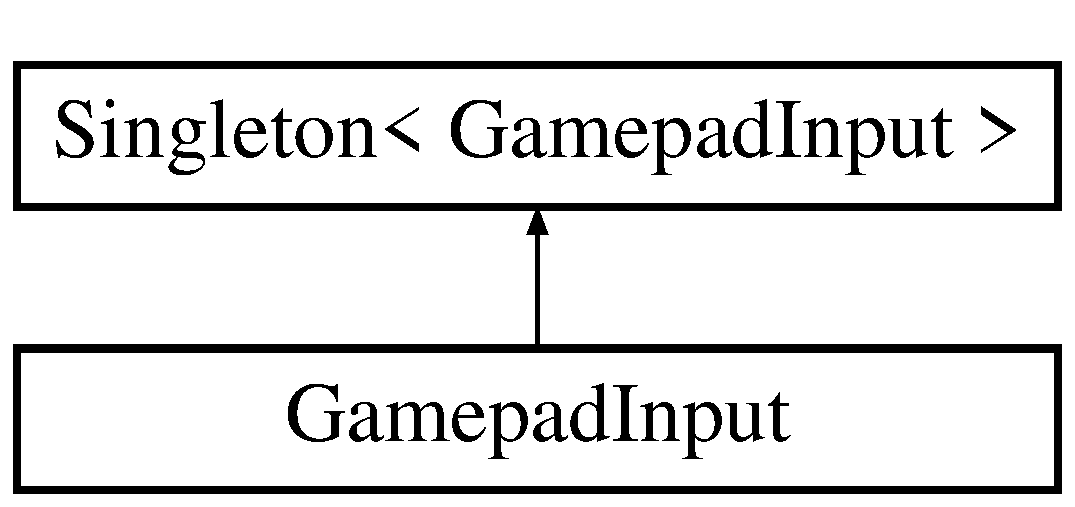
\includegraphics[height=2.000000cm]{class_gamepad_input}
\end{center}
\end{figure}
\subsection*{公開メンバ関数}
\begin{DoxyCompactItemize}
\item 
\mbox{\hyperlink{class_gamepad_input_acd9878326e438f379020827d63ebd6cf}{Gamepad\+Input}} ()
\begin{DoxyCompactList}\small\item\em コンストラクタで初期化 \end{DoxyCompactList}\item 
void \mbox{\hyperlink{class_gamepad_input_a3512c0cc4d57534c83db09c4b5377caa}{Update}} ()
\begin{DoxyCompactList}\small\item\em ゲームパッドインプットの更新 \end{DoxyCompactList}\item 
void \mbox{\hyperlink{class_gamepad_input_afd429d32d076130ff8a7df12037eaddd}{Vibration}} (size\+\_\+t index, float, float)
\begin{DoxyCompactList}\small\item\em コントローラーの振動 \end{DoxyCompactList}\item 
bool \mbox{\hyperlink{class_gamepad_input_a29a71d0503e038e55ffe282e2c768b05}{Get\+Button\+Down}} (size\+\_\+t index, \mbox{\hyperlink{gamepad__input_8h_a739845b0076428add52ca3cec492e705}{B\+U\+T\+T\+ON}} b) const
\begin{DoxyCompactList}\small\item\em --ゲッタ-- \end{DoxyCompactList}\item 
bool \mbox{\hyperlink{class_gamepad_input_a9a2f9042a5fa1c8e33fbd349f67747b3}{Get\+Button}} (size\+\_\+t index, \mbox{\hyperlink{gamepad__input_8h_a739845b0076428add52ca3cec492e705}{B\+U\+T\+T\+ON}} b) const
\begin{DoxyCompactList}\small\item\em ボタンを押しているかどうか \end{DoxyCompactList}\item 
bool \mbox{\hyperlink{class_gamepad_input_a5b76a114b8d3d03abbd2bcd91562109a}{Get\+Button\+Up}} (size\+\_\+t index, \mbox{\hyperlink{gamepad__input_8h_a739845b0076428add52ca3cec492e705}{B\+U\+T\+T\+ON}} b) const
\begin{DoxyCompactList}\small\item\em ボタンを離したかどうか \end{DoxyCompactList}\item 
float \mbox{\hyperlink{class_gamepad_input_a7e95e2a49cbd4729cf7156b9a703252a}{Get\+Trigger}} (size\+\_\+t index, const bool right) const
\begin{DoxyCompactList}\small\item\em トリガーの状態を返す \end{DoxyCompactList}\item 
float \mbox{\hyperlink{class_gamepad_input_a82333353a23ea0fa92bb87d6cf6592d8}{Get\+Stick}} (size\+\_\+t index, const bool right, const bool x) const
\begin{DoxyCompactList}\small\item\em スティックの状態を返す \end{DoxyCompactList}\end{DoxyCompactItemize}
\subsection*{その他の継承メンバ}


\subsection{詳解}
ゲームパッドのインプットクラス 

\subsection{構築子と解体子}
\mbox{\Hypertarget{class_gamepad_input_acd9878326e438f379020827d63ebd6cf}\label{class_gamepad_input_acd9878326e438f379020827d63ebd6cf}} 
\index{Gamepad\+Input@{Gamepad\+Input}!Gamepad\+Input@{Gamepad\+Input}}
\index{Gamepad\+Input@{Gamepad\+Input}!Gamepad\+Input@{Gamepad\+Input}}
\subsubsection{\texorpdfstring{Gamepad\+Input()}{GamepadInput()}}
{\footnotesize\ttfamily Gamepad\+Input\+::\+Gamepad\+Input (\begin{DoxyParamCaption}{ }\end{DoxyParamCaption})}



コンストラクタで初期化 



\subsection{関数詳解}
\mbox{\Hypertarget{class_gamepad_input_a9a2f9042a5fa1c8e33fbd349f67747b3}\label{class_gamepad_input_a9a2f9042a5fa1c8e33fbd349f67747b3}} 
\index{Gamepad\+Input@{Gamepad\+Input}!Get\+Button@{Get\+Button}}
\index{Get\+Button@{Get\+Button}!Gamepad\+Input@{Gamepad\+Input}}
\subsubsection{\texorpdfstring{Get\+Button()}{GetButton()}}
{\footnotesize\ttfamily bool Gamepad\+Input\+::\+Get\+Button (\begin{DoxyParamCaption}\item[{size\+\_\+t}]{index,  }\item[{\mbox{\hyperlink{gamepad__input_8h_a739845b0076428add52ca3cec492e705}{B\+U\+T\+T\+ON}}}]{b }\end{DoxyParamCaption}) const\hspace{0.3cm}{\ttfamily [inline]}}



ボタンを押しているかどうか 


\begin{DoxyParams}{引数}
{\em k} & 判定するボタン \\
\hline
\end{DoxyParams}
\mbox{\Hypertarget{class_gamepad_input_a29a71d0503e038e55ffe282e2c768b05}\label{class_gamepad_input_a29a71d0503e038e55ffe282e2c768b05}} 
\index{Gamepad\+Input@{Gamepad\+Input}!Get\+Button\+Down@{Get\+Button\+Down}}
\index{Get\+Button\+Down@{Get\+Button\+Down}!Gamepad\+Input@{Gamepad\+Input}}
\subsubsection{\texorpdfstring{Get\+Button\+Down()}{GetButtonDown()}}
{\footnotesize\ttfamily bool Gamepad\+Input\+::\+Get\+Button\+Down (\begin{DoxyParamCaption}\item[{size\+\_\+t}]{index,  }\item[{\mbox{\hyperlink{gamepad__input_8h_a739845b0076428add52ca3cec492e705}{B\+U\+T\+T\+ON}}}]{b }\end{DoxyParamCaption}) const\hspace{0.3cm}{\ttfamily [inline]}}



--ゲッタ-- 

ボタンを押したかどうか 
\begin{DoxyParams}{引数}
{\em k} & 判定するボタン \\
\hline
\end{DoxyParams}
\mbox{\Hypertarget{class_gamepad_input_a5b76a114b8d3d03abbd2bcd91562109a}\label{class_gamepad_input_a5b76a114b8d3d03abbd2bcd91562109a}} 
\index{Gamepad\+Input@{Gamepad\+Input}!Get\+Button\+Up@{Get\+Button\+Up}}
\index{Get\+Button\+Up@{Get\+Button\+Up}!Gamepad\+Input@{Gamepad\+Input}}
\subsubsection{\texorpdfstring{Get\+Button\+Up()}{GetButtonUp()}}
{\footnotesize\ttfamily bool Gamepad\+Input\+::\+Get\+Button\+Up (\begin{DoxyParamCaption}\item[{size\+\_\+t}]{index,  }\item[{\mbox{\hyperlink{gamepad__input_8h_a739845b0076428add52ca3cec492e705}{B\+U\+T\+T\+ON}}}]{b }\end{DoxyParamCaption}) const\hspace{0.3cm}{\ttfamily [inline]}}



ボタンを離したかどうか 


\begin{DoxyParams}{引数}
{\em k} & 判定するボタン \\
\hline
\end{DoxyParams}
\mbox{\Hypertarget{class_gamepad_input_a82333353a23ea0fa92bb87d6cf6592d8}\label{class_gamepad_input_a82333353a23ea0fa92bb87d6cf6592d8}} 
\index{Gamepad\+Input@{Gamepad\+Input}!Get\+Stick@{Get\+Stick}}
\index{Get\+Stick@{Get\+Stick}!Gamepad\+Input@{Gamepad\+Input}}
\subsubsection{\texorpdfstring{Get\+Stick()}{GetStick()}}
{\footnotesize\ttfamily float Gamepad\+Input\+::\+Get\+Stick (\begin{DoxyParamCaption}\item[{size\+\_\+t}]{index,  }\item[{const bool}]{right,  }\item[{const bool}]{x }\end{DoxyParamCaption}) const\hspace{0.3cm}{\ttfamily [inline]}}



スティックの状態を返す 


\begin{DoxyParams}{引数}
{\em right} & 判定するのが右かどうか \\
\hline
{\em right} & 判定するのがxかどうか \\
\hline
\end{DoxyParams}
\mbox{\Hypertarget{class_gamepad_input_a7e95e2a49cbd4729cf7156b9a703252a}\label{class_gamepad_input_a7e95e2a49cbd4729cf7156b9a703252a}} 
\index{Gamepad\+Input@{Gamepad\+Input}!Get\+Trigger@{Get\+Trigger}}
\index{Get\+Trigger@{Get\+Trigger}!Gamepad\+Input@{Gamepad\+Input}}
\subsubsection{\texorpdfstring{Get\+Trigger()}{GetTrigger()}}
{\footnotesize\ttfamily float Gamepad\+Input\+::\+Get\+Trigger (\begin{DoxyParamCaption}\item[{size\+\_\+t}]{index,  }\item[{const bool}]{right }\end{DoxyParamCaption}) const\hspace{0.3cm}{\ttfamily [inline]}}



トリガーの状態を返す 


\begin{DoxyParams}{引数}
{\em right} & 判定するのが右かどうか \\
\hline
\end{DoxyParams}
\mbox{\Hypertarget{class_gamepad_input_a3512c0cc4d57534c83db09c4b5377caa}\label{class_gamepad_input_a3512c0cc4d57534c83db09c4b5377caa}} 
\index{Gamepad\+Input@{Gamepad\+Input}!Update@{Update}}
\index{Update@{Update}!Gamepad\+Input@{Gamepad\+Input}}
\subsubsection{\texorpdfstring{Update()}{Update()}}
{\footnotesize\ttfamily void Gamepad\+Input\+::\+Update (\begin{DoxyParamCaption}{ }\end{DoxyParamCaption})}



ゲームパッドインプットの更新 

\mbox{\Hypertarget{class_gamepad_input_afd429d32d076130ff8a7df12037eaddd}\label{class_gamepad_input_afd429d32d076130ff8a7df12037eaddd}} 
\index{Gamepad\+Input@{Gamepad\+Input}!Vibration@{Vibration}}
\index{Vibration@{Vibration}!Gamepad\+Input@{Gamepad\+Input}}
\subsubsection{\texorpdfstring{Vibration()}{Vibration()}}
{\footnotesize\ttfamily void Gamepad\+Input\+::\+Vibration (\begin{DoxyParamCaption}\item[{size\+\_\+t}]{index,  }\item[{float}]{right,  }\item[{float}]{left }\end{DoxyParamCaption})}



コントローラーの振動 


\begin{DoxyParams}{引数}
{\em right} & 右のモーターの力 \\
\hline
{\em left} & 左のモーターの力 \\
\hline
\end{DoxyParams}


このクラス詳解は次のファイルから抽出されました\+:\begin{DoxyCompactItemize}
\item 
C\+:/\+Users/tokir/\+Documents/\+Git\+Hub/\+Weapon\+Merchant\+Adventure/src/src/input/gamepad/\mbox{\hyperlink{gamepad__input_8h}{gamepad\+\_\+input.\+h}}\item 
C\+:/\+Users/tokir/\+Documents/\+Git\+Hub/\+Weapon\+Merchant\+Adventure/src/src/input/gamepad/\mbox{\hyperlink{gamepad__input_8cpp}{gamepad\+\_\+input.\+cpp}}\end{DoxyCompactItemize}

\hypertarget{class_object}{}\section{Object クラス}
\label{class_object}\index{Object@{Object}}


オブジェクトのスーパークラス  




{\ttfamily \#include $<$object.\+h$>$}

\subsection*{公開メンバ関数}
\begin{DoxyCompactItemize}
\item 
virtual \mbox{\hyperlink{class_object_aa3e791419d84c4c346ef9499513b8e00}{$\sim$\+Object}} ()
\item 
virtual H\+R\+E\+S\+U\+LT \mbox{\hyperlink{class_object_a6e2cc01de0a4cf70bb779c059860eced}{Init}} ()=0
\item 
virtual void \mbox{\hyperlink{class_object_a5ee5c17a09981cbd7c469370e210b4ff}{Update}} ()=0
\item 
virtual void \mbox{\hyperlink{class_object_a19d531b9d8086ece15c228899ce456bf}{Render}} ()=0
\item 
virtual void \mbox{\hyperlink{class_object_acd8a6b7eebef988f20f6bf8c53d9b4bc}{Destroy}} ()=0
\end{DoxyCompactItemize}


\subsection{詳解}
オブジェクトのスーパークラス 

\subsection{構築子と解体子}
\mbox{\Hypertarget{class_object_aa3e791419d84c4c346ef9499513b8e00}\label{class_object_aa3e791419d84c4c346ef9499513b8e00}} 
\index{Object@{Object}!````~Object@{$\sim$\+Object}}
\index{````~Object@{$\sim$\+Object}!Object@{Object}}
\subsubsection{\texorpdfstring{$\sim$\+Object()}{~Object()}}
{\footnotesize\ttfamily virtual Object\+::$\sim$\+Object (\begin{DoxyParamCaption}{ }\end{DoxyParamCaption})\hspace{0.3cm}{\ttfamily [inline]}, {\ttfamily [virtual]}}



\subsection{関数詳解}
\mbox{\Hypertarget{class_object_acd8a6b7eebef988f20f6bf8c53d9b4bc}\label{class_object_acd8a6b7eebef988f20f6bf8c53d9b4bc}} 
\index{Object@{Object}!Destroy@{Destroy}}
\index{Destroy@{Destroy}!Object@{Object}}
\subsubsection{\texorpdfstring{Destroy()}{Destroy()}}
{\footnotesize\ttfamily virtual void Object\+::\+Destroy (\begin{DoxyParamCaption}{ }\end{DoxyParamCaption})\hspace{0.3cm}{\ttfamily [pure virtual]}}

\mbox{\Hypertarget{class_object_a6e2cc01de0a4cf70bb779c059860eced}\label{class_object_a6e2cc01de0a4cf70bb779c059860eced}} 
\index{Object@{Object}!Init@{Init}}
\index{Init@{Init}!Object@{Object}}
\subsubsection{\texorpdfstring{Init()}{Init()}}
{\footnotesize\ttfamily virtual H\+R\+E\+S\+U\+LT Object\+::\+Init (\begin{DoxyParamCaption}{ }\end{DoxyParamCaption})\hspace{0.3cm}{\ttfamily [pure virtual]}}

\mbox{\Hypertarget{class_object_a19d531b9d8086ece15c228899ce456bf}\label{class_object_a19d531b9d8086ece15c228899ce456bf}} 
\index{Object@{Object}!Render@{Render}}
\index{Render@{Render}!Object@{Object}}
\subsubsection{\texorpdfstring{Render()}{Render()}}
{\footnotesize\ttfamily virtual void Object\+::\+Render (\begin{DoxyParamCaption}{ }\end{DoxyParamCaption})\hspace{0.3cm}{\ttfamily [pure virtual]}}

\mbox{\Hypertarget{class_object_a5ee5c17a09981cbd7c469370e210b4ff}\label{class_object_a5ee5c17a09981cbd7c469370e210b4ff}} 
\index{Object@{Object}!Update@{Update}}
\index{Update@{Update}!Object@{Object}}
\subsubsection{\texorpdfstring{Update()}{Update()}}
{\footnotesize\ttfamily virtual void Object\+::\+Update (\begin{DoxyParamCaption}{ }\end{DoxyParamCaption})\hspace{0.3cm}{\ttfamily [pure virtual]}}



このクラス詳解は次のファイルから抽出されました\+:\begin{DoxyCompactItemize}
\item 
C\+:/\+Users/tokir/\+Documents/\+Git\+Hub/\+Weapon\+Merchant\+Adventure/src/object/\mbox{\hyperlink{object_8h}{object.\+h}}\end{DoxyCompactItemize}

\hypertarget{class_scene}{}\section{Scene クラス}
\label{class_scene}\index{Scene@{Scene}}


マネージャーを含まないシーンのスーパークラス  




{\ttfamily \#include $<$scene.\+h$>$}

Scene の継承関係図\begin{figure}[H]
\begin{center}
\leavevmode
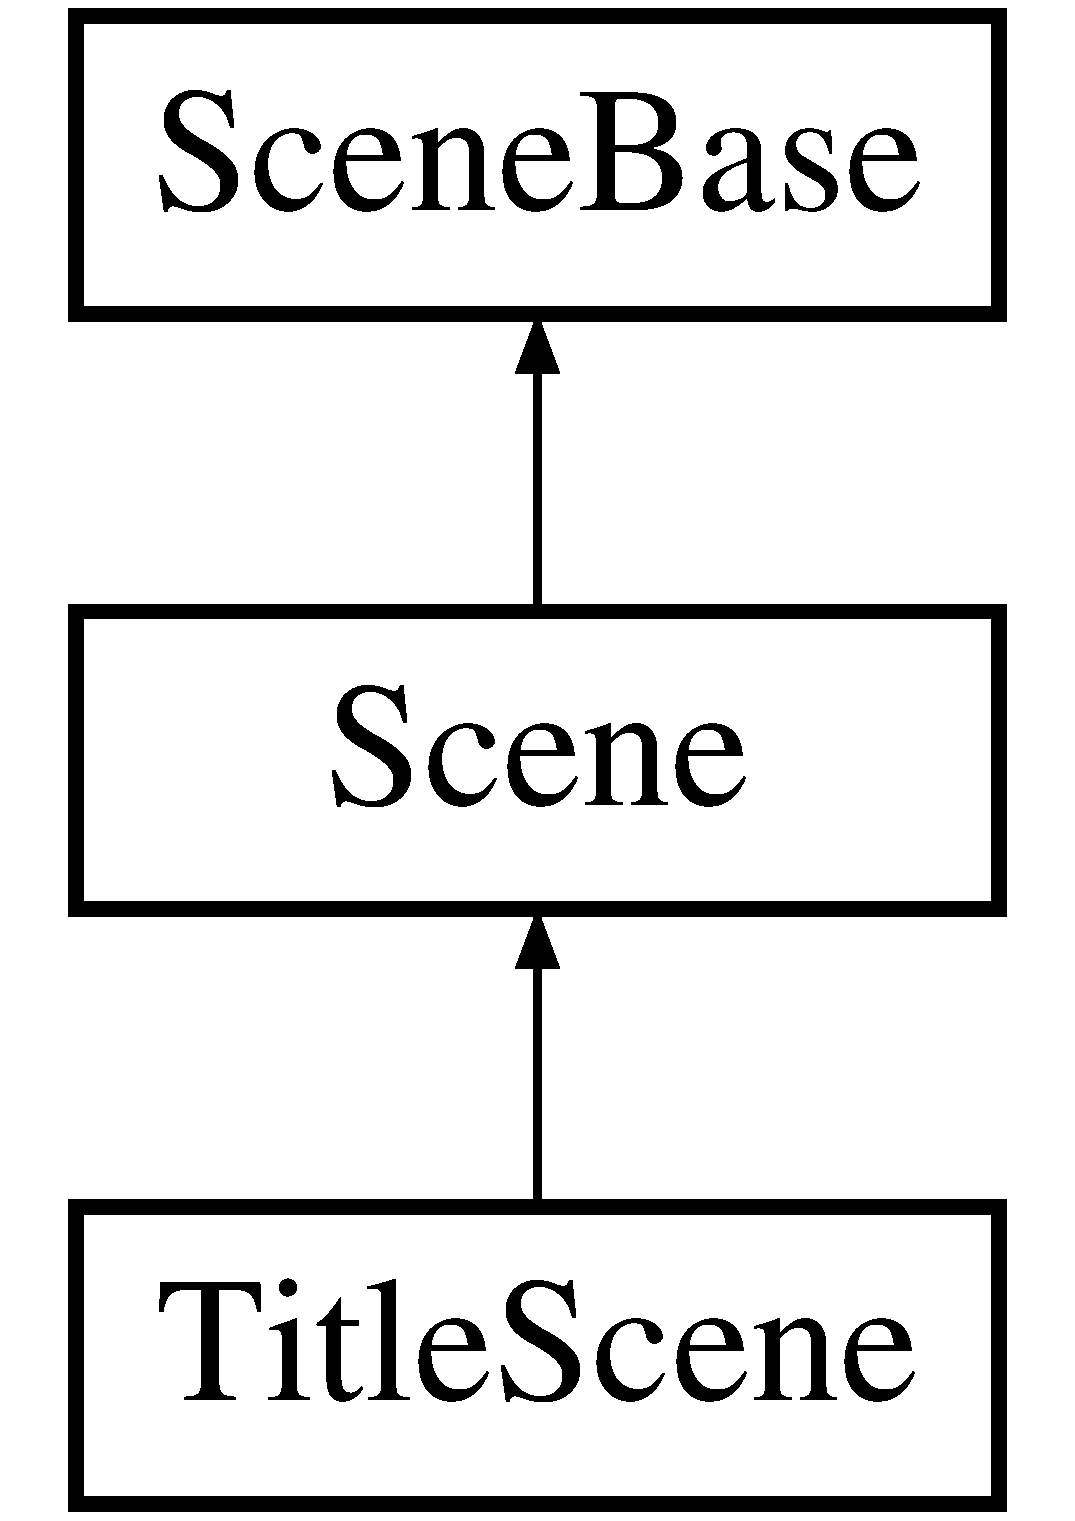
\includegraphics[height=1.875000cm]{class_scene}
\end{center}
\end{figure}
\subsection*{公開メンバ関数}
\begin{DoxyCompactItemize}
\item 
virtual \mbox{\hyperlink{class_scene_aa0a5be58e2ee2d1fdafc5fb46b5e661e}{$\sim$\+Scene}} ()
\item 
virtual std\+::shared\+\_\+ptr$<$ \mbox{\hyperlink{class_scene}{Scene}} $>$ \mbox{\hyperlink{class_scene_ab71ee5f19764b90c87b4574aa1cb1d25}{Update}} (std\+::shared\+\_\+ptr$<$ \mbox{\hyperlink{class_scene}{Scene}} $>$ \&)=0
\item 
virtual void \mbox{\hyperlink{class_scene_ad19a449c6ed452823dae14183689570c}{Exit\+Fade\+Update}} ()
\begin{DoxyCompactList}\small\item\em シーンが変わるときの更新 \end{DoxyCompactList}\end{DoxyCompactItemize}


\subsection{詳解}
マネージャーを含まないシーンのスーパークラス 

マネージャーはこのクラスを保持する 

\subsection{構築子と解体子}
\mbox{\Hypertarget{class_scene_aa0a5be58e2ee2d1fdafc5fb46b5e661e}\label{class_scene_aa0a5be58e2ee2d1fdafc5fb46b5e661e}} 
\index{Scene@{Scene}!````~Scene@{$\sim$\+Scene}}
\index{````~Scene@{$\sim$\+Scene}!Scene@{Scene}}
\subsubsection{\texorpdfstring{$\sim$\+Scene()}{~Scene()}}
{\footnotesize\ttfamily virtual Scene\+::$\sim$\+Scene (\begin{DoxyParamCaption}{ }\end{DoxyParamCaption})\hspace{0.3cm}{\ttfamily [inline]}, {\ttfamily [virtual]}}



\subsection{関数詳解}
\mbox{\Hypertarget{class_scene_ad19a449c6ed452823dae14183689570c}\label{class_scene_ad19a449c6ed452823dae14183689570c}} 
\index{Scene@{Scene}!Exit\+Fade\+Update@{Exit\+Fade\+Update}}
\index{Exit\+Fade\+Update@{Exit\+Fade\+Update}!Scene@{Scene}}
\subsubsection{\texorpdfstring{Exit\+Fade\+Update()}{ExitFadeUpdate()}}
{\footnotesize\ttfamily virtual void Scene\+::\+Exit\+Fade\+Update (\begin{DoxyParamCaption}{ }\end{DoxyParamCaption})\hspace{0.3cm}{\ttfamily [inline]}, {\ttfamily [virtual]}}



シーンが変わるときの更新 



\mbox{\hyperlink{class_select_scene_a546190bc143f6d7a3055935f97b55596}{Select\+Scene}}で再実装されています。

\mbox{\Hypertarget{class_scene_ab71ee5f19764b90c87b4574aa1cb1d25}\label{class_scene_ab71ee5f19764b90c87b4574aa1cb1d25}} 
\index{Scene@{Scene}!Update@{Update}}
\index{Update@{Update}!Scene@{Scene}}
\subsubsection{\texorpdfstring{Update()}{Update()}}
{\footnotesize\ttfamily virtual std\+::shared\+\_\+ptr$<$\mbox{\hyperlink{class_scene}{Scene}}$>$ Scene\+::\+Update (\begin{DoxyParamCaption}\item[{std\+::shared\+\_\+ptr$<$ \mbox{\hyperlink{class_scene}{Scene}} $>$ \&}]{ }\end{DoxyParamCaption})\hspace{0.3cm}{\ttfamily [pure virtual]}}



\mbox{\hyperlink{class_select_scene_a0cef696ddf74155e061cc5f9f2e06419}{Select\+Scene}}, \mbox{\hyperlink{class_title_scene_ab3097e96e2fe65d6fad0d6bb45a14f9f}{Title\+Scene}}, \mbox{\hyperlink{class_pause_scene_a6adfe0685eb6bc64e658f6364c9f704d}{Pause\+Scene}}, \mbox{\hyperlink{class_game_scene_easy_ac2bccbf61722010fd6f317693ee7b8b1}{Game\+Scene\+Easy}}, \mbox{\hyperlink{class_game_scene_hard_ac132a0e281a7d4e6b71deb6e5bcfdb9d}{Game\+Scene\+Hard}}, \mbox{\hyperlink{class_game_scene_normal_a3e45ac3882f1d0dd5c77ab4f0a1ccb33}{Game\+Scene\+Normal}}, \mbox{\hyperlink{class_exit_scene_a18655f3124150a911f266e66e3fc4480}{Exit\+Scene}}で実装されています。



このクラス詳解は次のファイルから抽出されました\+:\begin{DoxyCompactItemize}
\item 
C\+:/\+Users/tokir/\+Documents/\+Git\+Hub/\+Weapon\+Merchant\+Adventure/src/src/scene/\mbox{\hyperlink{scene_8h}{scene.\+h}}\end{DoxyCompactItemize}

\hypertarget{class_scene_base}{}\section{Scene\+Base クラス}
\label{class_scene_base}\index{Scene\+Base@{Scene\+Base}}


マネージャーを含むシーンのスーパークラス  




{\ttfamily \#include $<$scene\+\_\+base.\+h$>$}

Scene\+Base の継承関係図\begin{figure}[H]
\begin{center}
\leavevmode
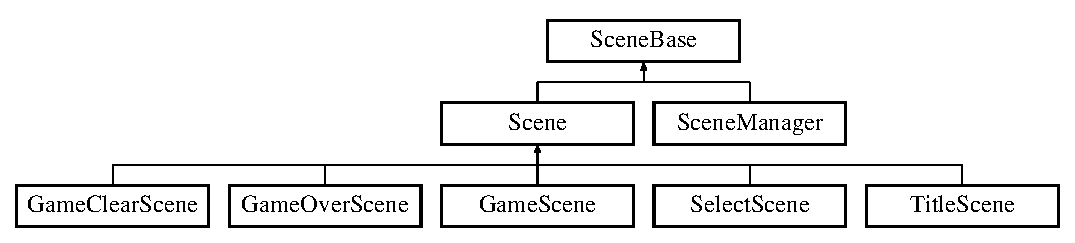
\includegraphics[height=3.000000cm]{class_scene_base}
\end{center}
\end{figure}
\subsection*{公開メンバ関数}
\begin{DoxyCompactItemize}
\item 
virtual \mbox{\hyperlink{class_scene_base_a187dd160e5a16909bcc6529851e38318}{$\sim$\+Scene\+Base}} ()
\item 
virtual void \mbox{\hyperlink{class_scene_base_a24d7db43c819924dc8b07b436f6d3148}{Init}} ()=0
\item 
virtual void \mbox{\hyperlink{class_scene_base_ad981674ce731ea267f398e889bbb9dc3}{Render}} ()=0
\item 
virtual void \mbox{\hyperlink{class_scene_base_a7c5b54020bc519b4dadfe9770d6b27f7}{Destroy}} ()=0
\end{DoxyCompactItemize}
\subsection*{限定公開変数類}
\begin{DoxyCompactItemize}
\item 
\mbox{\hyperlink{scene__base_8h_a24cee5343fb9d0706ead6e8601f363be}{S\+C\+E\+NE}} \mbox{\hyperlink{class_scene_base_a18dcdbacfbd98f73099c3cbeb70ae3b8}{my\+\_\+scene}}
\end{DoxyCompactItemize}


\subsection{詳解}
マネージャーを含むシーンのスーパークラス 

\subsection{構築子と解体子}
\mbox{\Hypertarget{class_scene_base_a187dd160e5a16909bcc6529851e38318}\label{class_scene_base_a187dd160e5a16909bcc6529851e38318}} 
\index{Scene\+Base@{Scene\+Base}!````~Scene\+Base@{$\sim$\+Scene\+Base}}
\index{````~Scene\+Base@{$\sim$\+Scene\+Base}!Scene\+Base@{Scene\+Base}}
\subsubsection{\texorpdfstring{$\sim$\+Scene\+Base()}{~SceneBase()}}
{\footnotesize\ttfamily virtual Scene\+Base\+::$\sim$\+Scene\+Base (\begin{DoxyParamCaption}{ }\end{DoxyParamCaption})\hspace{0.3cm}{\ttfamily [inline]}, {\ttfamily [virtual]}}



\subsection{関数詳解}
\mbox{\Hypertarget{class_scene_base_a7c5b54020bc519b4dadfe9770d6b27f7}\label{class_scene_base_a7c5b54020bc519b4dadfe9770d6b27f7}} 
\index{Scene\+Base@{Scene\+Base}!Destroy@{Destroy}}
\index{Destroy@{Destroy}!Scene\+Base@{Scene\+Base}}
\subsubsection{\texorpdfstring{Destroy()}{Destroy()}}
{\footnotesize\ttfamily virtual void Scene\+Base\+::\+Destroy (\begin{DoxyParamCaption}{ }\end{DoxyParamCaption})\hspace{0.3cm}{\ttfamily [pure virtual]}}



\mbox{\hyperlink{class_title_scene_adfbc5f934572ede2e36419b089c88fe8}{Title\+Scene}}, \mbox{\hyperlink{class_scene_manager_a0e3ad11342e763f0d4108c0b4674a157}{Scene\+Manager}}で実装されています。

\mbox{\Hypertarget{class_scene_base_a24d7db43c819924dc8b07b436f6d3148}\label{class_scene_base_a24d7db43c819924dc8b07b436f6d3148}} 
\index{Scene\+Base@{Scene\+Base}!Init@{Init}}
\index{Init@{Init}!Scene\+Base@{Scene\+Base}}
\subsubsection{\texorpdfstring{Init()}{Init()}}
{\footnotesize\ttfamily virtual void Scene\+Base\+::\+Init (\begin{DoxyParamCaption}{ }\end{DoxyParamCaption})\hspace{0.3cm}{\ttfamily [pure virtual]}}



\mbox{\hyperlink{class_title_scene_a3d039e7db0fa1e22e8c36d3cedfbd318}{Title\+Scene}}, \mbox{\hyperlink{class_scene_manager_a6c0e84d0e76f23fb3172839dba5f091b}{Scene\+Manager}}で実装されています。

\mbox{\Hypertarget{class_scene_base_ad981674ce731ea267f398e889bbb9dc3}\label{class_scene_base_ad981674ce731ea267f398e889bbb9dc3}} 
\index{Scene\+Base@{Scene\+Base}!Render@{Render}}
\index{Render@{Render}!Scene\+Base@{Scene\+Base}}
\subsubsection{\texorpdfstring{Render()}{Render()}}
{\footnotesize\ttfamily virtual void Scene\+Base\+::\+Render (\begin{DoxyParamCaption}{ }\end{DoxyParamCaption})\hspace{0.3cm}{\ttfamily [pure virtual]}}



\mbox{\hyperlink{class_title_scene_af12c59b3bf9458640938c5ca620527ae}{Title\+Scene}}, \mbox{\hyperlink{class_scene_manager_a968ae7a0065b793f139bda6bcc58d106}{Scene\+Manager}}で実装されています。



\subsection{メンバ詳解}
\mbox{\Hypertarget{class_scene_base_a18dcdbacfbd98f73099c3cbeb70ae3b8}\label{class_scene_base_a18dcdbacfbd98f73099c3cbeb70ae3b8}} 
\index{Scene\+Base@{Scene\+Base}!my\+\_\+scene@{my\+\_\+scene}}
\index{my\+\_\+scene@{my\+\_\+scene}!Scene\+Base@{Scene\+Base}}
\subsubsection{\texorpdfstring{my\+\_\+scene}{my\_scene}}
{\footnotesize\ttfamily \mbox{\hyperlink{scene__base_8h_a24cee5343fb9d0706ead6e8601f363be}{S\+C\+E\+NE}} Scene\+Base\+::my\+\_\+scene\hspace{0.3cm}{\ttfamily [protected]}}



このクラス詳解は次のファイルから抽出されました\+:\begin{DoxyCompactItemize}
\item 
C\+:/\+Users/tokir/\+Documents/\+Git\+Hub/\+Weapon\+Merchant\+Adventure/src/scene/base/\mbox{\hyperlink{scene__base_8h}{scene\+\_\+base.\+h}}\end{DoxyCompactItemize}

\hypertarget{class_scene_manager}{}\section{Scene\+Manager クラス}
\label{class_scene_manager}\index{Scene\+Manager@{Scene\+Manager}}


シーンをマネージャーするクラス  




{\ttfamily \#include $<$scene\+\_\+manager.\+h$>$}

Scene\+Manager の継承関係図\begin{figure}[H]
\begin{center}
\leavevmode
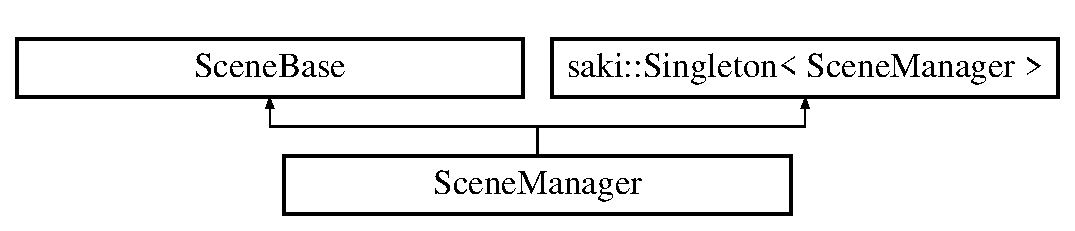
\includegraphics[height=2.000000cm]{class_scene_manager}
\end{center}
\end{figure}
\subsection*{公開メンバ関数}
\begin{DoxyCompactItemize}
\item 
void \mbox{\hyperlink{class_scene_manager_a6c0e84d0e76f23fb3172839dba5f091b}{Init}} () final
\begin{DoxyCompactList}\small\item\em シーンマネージャーの初期化 \end{DoxyCompactList}\item 
void \mbox{\hyperlink{class_scene_manager_a63dcf65832d6a2c190bf496d9a3b00a3}{Update}} ()
\begin{DoxyCompactList}\small\item\em 保持してるシーンの更新 \end{DoxyCompactList}\item 
void \mbox{\hyperlink{class_scene_manager_a968ae7a0065b793f139bda6bcc58d106}{Render}} () final
\begin{DoxyCompactList}\small\item\em 保持してるシーンの描画 \end{DoxyCompactList}\item 
void \mbox{\hyperlink{class_scene_manager_a0e3ad11342e763f0d4108c0b4674a157}{Destroy}} () final
\begin{DoxyCompactList}\small\item\em 保持してるシーンのマネージャーの破棄 \end{DoxyCompactList}\item 
void \mbox{\hyperlink{class_scene_manager_a5ed223ec14c6b62d378b3f95ed4f5d8e}{Continue\+Game}} (std\+::shared\+\_\+ptr$<$ \mbox{\hyperlink{class_scene}{Scene}} $>$ \&p)
\end{DoxyCompactItemize}
\subsection*{公開変数類}
\begin{DoxyCompactItemize}
\item 
bool \mbox{\hyperlink{class_scene_manager_a416645f4b11ce8cdb81d9d43d1c5666b}{is\+\_\+game\+\_\+scene}} = false
\end{DoxyCompactItemize}
\subsection*{その他の継承メンバ}


\subsection{詳解}
シーンをマネージャーするクラス 

\subsection{関数詳解}
\mbox{\Hypertarget{class_scene_manager_a5ed223ec14c6b62d378b3f95ed4f5d8e}\label{class_scene_manager_a5ed223ec14c6b62d378b3f95ed4f5d8e}} 
\index{Scene\+Manager@{Scene\+Manager}!Continue\+Game@{Continue\+Game}}
\index{Continue\+Game@{Continue\+Game}!Scene\+Manager@{Scene\+Manager}}
\subsubsection{\texorpdfstring{Continue\+Game()}{ContinueGame()}}
{\footnotesize\ttfamily void Scene\+Manager\+::\+Continue\+Game (\begin{DoxyParamCaption}\item[{std\+::shared\+\_\+ptr$<$ \mbox{\hyperlink{class_scene}{Scene}} $>$ \&}]{p }\end{DoxyParamCaption})\hspace{0.3cm}{\ttfamily [inline]}}

\mbox{\Hypertarget{class_scene_manager_a0e3ad11342e763f0d4108c0b4674a157}\label{class_scene_manager_a0e3ad11342e763f0d4108c0b4674a157}} 
\index{Scene\+Manager@{Scene\+Manager}!Destroy@{Destroy}}
\index{Destroy@{Destroy}!Scene\+Manager@{Scene\+Manager}}
\subsubsection{\texorpdfstring{Destroy()}{Destroy()}}
{\footnotesize\ttfamily void Scene\+Manager\+::\+Destroy (\begin{DoxyParamCaption}{ }\end{DoxyParamCaption})\hspace{0.3cm}{\ttfamily [final]}, {\ttfamily [virtual]}}



保持してるシーンのマネージャーの破棄 



\mbox{\hyperlink{class_scene_base_a7c5b54020bc519b4dadfe9770d6b27f7}{Scene\+Base}}を実装しています。

\mbox{\Hypertarget{class_scene_manager_a6c0e84d0e76f23fb3172839dba5f091b}\label{class_scene_manager_a6c0e84d0e76f23fb3172839dba5f091b}} 
\index{Scene\+Manager@{Scene\+Manager}!Init@{Init}}
\index{Init@{Init}!Scene\+Manager@{Scene\+Manager}}
\subsubsection{\texorpdfstring{Init()}{Init()}}
{\footnotesize\ttfamily void Scene\+Manager\+::\+Init (\begin{DoxyParamCaption}{ }\end{DoxyParamCaption})\hspace{0.3cm}{\ttfamily [final]}, {\ttfamily [virtual]}}



シーンマネージャーの初期化 



\mbox{\hyperlink{class_scene_base_a24d7db43c819924dc8b07b436f6d3148}{Scene\+Base}}を実装しています。

\mbox{\Hypertarget{class_scene_manager_a968ae7a0065b793f139bda6bcc58d106}\label{class_scene_manager_a968ae7a0065b793f139bda6bcc58d106}} 
\index{Scene\+Manager@{Scene\+Manager}!Render@{Render}}
\index{Render@{Render}!Scene\+Manager@{Scene\+Manager}}
\subsubsection{\texorpdfstring{Render()}{Render()}}
{\footnotesize\ttfamily void Scene\+Manager\+::\+Render (\begin{DoxyParamCaption}{ }\end{DoxyParamCaption})\hspace{0.3cm}{\ttfamily [final]}, {\ttfamily [virtual]}}



保持してるシーンの描画 



\mbox{\hyperlink{class_scene_base_ad981674ce731ea267f398e889bbb9dc3}{Scene\+Base}}を実装しています。

\mbox{\Hypertarget{class_scene_manager_a63dcf65832d6a2c190bf496d9a3b00a3}\label{class_scene_manager_a63dcf65832d6a2c190bf496d9a3b00a3}} 
\index{Scene\+Manager@{Scene\+Manager}!Update@{Update}}
\index{Update@{Update}!Scene\+Manager@{Scene\+Manager}}
\subsubsection{\texorpdfstring{Update()}{Update()}}
{\footnotesize\ttfamily void Scene\+Manager\+::\+Update (\begin{DoxyParamCaption}{ }\end{DoxyParamCaption})}



保持してるシーンの更新 



\subsection{メンバ詳解}
\mbox{\Hypertarget{class_scene_manager_a416645f4b11ce8cdb81d9d43d1c5666b}\label{class_scene_manager_a416645f4b11ce8cdb81d9d43d1c5666b}} 
\index{Scene\+Manager@{Scene\+Manager}!is\+\_\+game\+\_\+scene@{is\+\_\+game\+\_\+scene}}
\index{is\+\_\+game\+\_\+scene@{is\+\_\+game\+\_\+scene}!Scene\+Manager@{Scene\+Manager}}
\subsubsection{\texorpdfstring{is\+\_\+game\+\_\+scene}{is\_game\_scene}}
{\footnotesize\ttfamily bool Scene\+Manager\+::is\+\_\+game\+\_\+scene = false}



このクラス詳解は次のファイルから抽出されました\+:\begin{DoxyCompactItemize}
\item 
C\+:/\+Users/tokir/\+Documents/\+Git\+Hub/\+Weapon\+Merchant\+Adventure/src/src/scene/manager/\mbox{\hyperlink{scene__manager_8h}{scene\+\_\+manager.\+h}}\item 
C\+:/\+Users/tokir/\+Documents/\+Git\+Hub/\+Weapon\+Merchant\+Adventure/src/src/scene/manager/\mbox{\hyperlink{scene__manager_8cpp}{scene\+\_\+manager.\+cpp}}\end{DoxyCompactItemize}

\hypertarget{class_singleton}{}\section{Singleton$<$ T $>$ クラステンプレート}
\label{class_singleton}\index{Singleton$<$ T $>$@{Singleton$<$ T $>$}}


Singletonテンプレートスーパークラス  




{\ttfamily \#include $<$singleton.\+h$>$}

\subsection*{公開メンバ関数}
\begin{DoxyCompactItemize}
\item 
virtual \mbox{\hyperlink{class_singleton_ad3c93143836479fb3dd96b21b795938c}{$\sim$\+Singleton}} ()
\end{DoxyCompactItemize}
\subsection*{静的公開メンバ関数}
\begin{DoxyCompactItemize}
\item 
static std\+::unique\+\_\+ptr$<$ T $>$ \& \mbox{\hyperlink{class_singleton_a57b10e4aa6d89bbac3a16355914655b3}{Get\+Instance}} ()
\begin{DoxyCompactList}\small\item\em インスタンスの取得 \end{DoxyCompactList}\end{DoxyCompactItemize}
\subsection*{限定公開メンバ関数}
\begin{DoxyCompactItemize}
\item 
\mbox{\hyperlink{class_singleton_a923b995920da9c06590adb170ab2f890}{Singleton}} ()
\end{DoxyCompactItemize}


\subsection{詳解}
\subsubsection*{template$<$typename T$>$\newline
class Singleton$<$ T $>$}

Singletonテンプレートスーパークラス 

publicで仮引数にそのクラスを入れて継承するとそのクラスが\+Singletonになる 

\subsection{構築子と解体子}
\mbox{\Hypertarget{class_singleton_ad3c93143836479fb3dd96b21b795938c}\label{class_singleton_ad3c93143836479fb3dd96b21b795938c}} 
\index{Singleton@{Singleton}!````~Singleton@{$\sim$\+Singleton}}
\index{````~Singleton@{$\sim$\+Singleton}!Singleton@{Singleton}}
\subsubsection{\texorpdfstring{$\sim$\+Singleton()}{~Singleton()}}
{\footnotesize\ttfamily template$<$typename T$>$ \\
virtual \mbox{\hyperlink{class_singleton}{Singleton}}$<$ T $>$\+::$\sim$\mbox{\hyperlink{class_singleton}{Singleton}} (\begin{DoxyParamCaption}{ }\end{DoxyParamCaption})\hspace{0.3cm}{\ttfamily [inline]}, {\ttfamily [virtual]}}

\mbox{\Hypertarget{class_singleton_a923b995920da9c06590adb170ab2f890}\label{class_singleton_a923b995920da9c06590adb170ab2f890}} 
\index{Singleton@{Singleton}!Singleton@{Singleton}}
\index{Singleton@{Singleton}!Singleton@{Singleton}}
\subsubsection{\texorpdfstring{Singleton()}{Singleton()}}
{\footnotesize\ttfamily template$<$typename T$>$ \\
\mbox{\hyperlink{class_singleton}{Singleton}}$<$ T $>$\+::\mbox{\hyperlink{class_singleton}{Singleton}} (\begin{DoxyParamCaption}{ }\end{DoxyParamCaption})\hspace{0.3cm}{\ttfamily [inline]}, {\ttfamily [protected]}}



\subsection{関数詳解}
\mbox{\Hypertarget{class_singleton_a57b10e4aa6d89bbac3a16355914655b3}\label{class_singleton_a57b10e4aa6d89bbac3a16355914655b3}} 
\index{Singleton@{Singleton}!Get\+Instance@{Get\+Instance}}
\index{Get\+Instance@{Get\+Instance}!Singleton@{Singleton}}
\subsubsection{\texorpdfstring{Get\+Instance()}{GetInstance()}}
{\footnotesize\ttfamily template$<$typename T$>$ \\
static std\+::unique\+\_\+ptr$<$T$>$\& \mbox{\hyperlink{class_singleton}{Singleton}}$<$ T $>$\+::Get\+Instance (\begin{DoxyParamCaption}{ }\end{DoxyParamCaption})\hspace{0.3cm}{\ttfamily [inline]}, {\ttfamily [static]}}



インスタンスの取得 

\begin{DoxyReturn}{戻り値}
std\+::unique\+\_\+ptr$<$\+T$>$\& インスタンス 
\end{DoxyReturn}


このクラス詳解は次のファイルから抽出されました\+:\begin{DoxyCompactItemize}
\item 
C\+:/\+Users/tokir/\+Documents/\+Git\+Hub/\+Weapon\+Merchant\+Adventure/src/common/\mbox{\hyperlink{singleton_8h}{singleton.\+h}}\end{DoxyCompactItemize}

\hypertarget{class_sound}{}\section{Sound クラス}
\label{class_sound}\index{Sound@{Sound}}


 個々のサウンドクラス  




{\ttfamily \#include $<$sound.\+h$>$}

\subsection*{公開メンバ関数}
\begin{DoxyCompactItemize}
\item 
void \mbox{\hyperlink{class_sound_a3c8007c8e52bf541fc81adfa4b340b0f}{Init}} (W\+C\+H\+AR $\ast$, bool, bool)
\begin{DoxyCompactList}\small\item\em サウンドの初期化 \end{DoxyCompactList}\item 
void \mbox{\hyperlink{class_sound_ae021b518e93d7d8c6f3ea951cd4b98d8}{Start}} ()
\item 
void \mbox{\hyperlink{class_sound_a188de6836d531813da378464e392e813}{Stop}} ()
\item 
void \mbox{\hyperlink{class_sound_a4e199b4346519a4977fe94998c4a77e7}{Pause}} ()
\item 
void \mbox{\hyperlink{class_sound_a993eee69f61611ca1b4621ea0952e2c8}{Set\+Volume}} (float vol)
\item 
void \mbox{\hyperlink{class_sound_a06b9680efb2b6b41b52d9f25ac0264f1}{Set\+Pitch}} (float pit)
\item 
void \mbox{\hyperlink{class_sound_a1b066e78405656b1475849139ca24dce}{Set\+Pan}} (float pan)
\item 
\mbox{\hyperlink{class_sound_a0907389078bf740be2a5763366ad3376}{$\sim$\+Sound}} ()
\begin{DoxyCompactList}\small\item\em デストラクタ \end{DoxyCompactList}\item 
std\+::unique\+\_\+ptr$<$ Direct\+X\+::\+Sound\+Effect\+Instance $>$ \& \mbox{\hyperlink{class_sound_a0d79b20f421c0020c53b08c05b6df25b}{operator()}} ()
\end{DoxyCompactItemize}


\subsection{詳解}
 個々のサウンドクラス 

\subsection{構築子と解体子}
\mbox{\Hypertarget{class_sound_a0907389078bf740be2a5763366ad3376}\label{class_sound_a0907389078bf740be2a5763366ad3376}} 
\index{Sound@{Sound}!````~Sound@{$\sim$\+Sound}}
\index{````~Sound@{$\sim$\+Sound}!Sound@{Sound}}
\subsubsection{\texorpdfstring{$\sim$\+Sound()}{~Sound()}}
{\footnotesize\ttfamily Sound\+::$\sim$\+Sound (\begin{DoxyParamCaption}{ }\end{DoxyParamCaption})}



デストラクタ 



\subsection{関数詳解}
\mbox{\Hypertarget{class_sound_a3c8007c8e52bf541fc81adfa4b340b0f}\label{class_sound_a3c8007c8e52bf541fc81adfa4b340b0f}} 
\index{Sound@{Sound}!Init@{Init}}
\index{Init@{Init}!Sound@{Sound}}
\subsubsection{\texorpdfstring{Init()}{Init()}}
{\footnotesize\ttfamily void Sound\+::\+Init (\begin{DoxyParamCaption}\item[{W\+C\+H\+AR $\ast$}]{path,  }\item[{bool}]{loop,  }\item[{bool}]{awake }\end{DoxyParamCaption})}



サウンドの初期化 


\begin{DoxyParams}{引数}
{\em path} & サウンドのパス \\
\hline
{\em loop} & ループするかどうか \\
\hline
{\em awake} & 初期化した瞬間から再生するかどうか \\
\hline
\end{DoxyParams}
\mbox{\Hypertarget{class_sound_a0d79b20f421c0020c53b08c05b6df25b}\label{class_sound_a0d79b20f421c0020c53b08c05b6df25b}} 
\index{Sound@{Sound}!operator()@{operator()}}
\index{operator()@{operator()}!Sound@{Sound}}
\subsubsection{\texorpdfstring{operator()()}{operator()()}}
{\footnotesize\ttfamily std\+::unique\+\_\+ptr$<$Direct\+X\+::\+Sound\+Effect\+Instance$>$\& Sound\+::operator() (\begin{DoxyParamCaption}{ }\end{DoxyParamCaption})\hspace{0.3cm}{\ttfamily [inline]}}

\mbox{\Hypertarget{class_sound_a4e199b4346519a4977fe94998c4a77e7}\label{class_sound_a4e199b4346519a4977fe94998c4a77e7}} 
\index{Sound@{Sound}!Pause@{Pause}}
\index{Pause@{Pause}!Sound@{Sound}}
\subsubsection{\texorpdfstring{Pause()}{Pause()}}
{\footnotesize\ttfamily void Sound\+::\+Pause (\begin{DoxyParamCaption}{ }\end{DoxyParamCaption})\hspace{0.3cm}{\ttfamily [inline]}}

\mbox{\Hypertarget{class_sound_a1b066e78405656b1475849139ca24dce}\label{class_sound_a1b066e78405656b1475849139ca24dce}} 
\index{Sound@{Sound}!Set\+Pan@{Set\+Pan}}
\index{Set\+Pan@{Set\+Pan}!Sound@{Sound}}
\subsubsection{\texorpdfstring{Set\+Pan()}{SetPan()}}
{\footnotesize\ttfamily void Sound\+::\+Set\+Pan (\begin{DoxyParamCaption}\item[{float}]{pan }\end{DoxyParamCaption})\hspace{0.3cm}{\ttfamily [inline]}}

\mbox{\Hypertarget{class_sound_a06b9680efb2b6b41b52d9f25ac0264f1}\label{class_sound_a06b9680efb2b6b41b52d9f25ac0264f1}} 
\index{Sound@{Sound}!Set\+Pitch@{Set\+Pitch}}
\index{Set\+Pitch@{Set\+Pitch}!Sound@{Sound}}
\subsubsection{\texorpdfstring{Set\+Pitch()}{SetPitch()}}
{\footnotesize\ttfamily void Sound\+::\+Set\+Pitch (\begin{DoxyParamCaption}\item[{float}]{pit }\end{DoxyParamCaption})\hspace{0.3cm}{\ttfamily [inline]}}

\mbox{\Hypertarget{class_sound_a993eee69f61611ca1b4621ea0952e2c8}\label{class_sound_a993eee69f61611ca1b4621ea0952e2c8}} 
\index{Sound@{Sound}!Set\+Volume@{Set\+Volume}}
\index{Set\+Volume@{Set\+Volume}!Sound@{Sound}}
\subsubsection{\texorpdfstring{Set\+Volume()}{SetVolume()}}
{\footnotesize\ttfamily void Sound\+::\+Set\+Volume (\begin{DoxyParamCaption}\item[{float}]{vol }\end{DoxyParamCaption})\hspace{0.3cm}{\ttfamily [inline]}}

\mbox{\Hypertarget{class_sound_ae021b518e93d7d8c6f3ea951cd4b98d8}\label{class_sound_ae021b518e93d7d8c6f3ea951cd4b98d8}} 
\index{Sound@{Sound}!Start@{Start}}
\index{Start@{Start}!Sound@{Sound}}
\subsubsection{\texorpdfstring{Start()}{Start()}}
{\footnotesize\ttfamily void Sound\+::\+Start (\begin{DoxyParamCaption}{ }\end{DoxyParamCaption})\hspace{0.3cm}{\ttfamily [inline]}}

\mbox{\Hypertarget{class_sound_a188de6836d531813da378464e392e813}\label{class_sound_a188de6836d531813da378464e392e813}} 
\index{Sound@{Sound}!Stop@{Stop}}
\index{Stop@{Stop}!Sound@{Sound}}
\subsubsection{\texorpdfstring{Stop()}{Stop()}}
{\footnotesize\ttfamily void Sound\+::\+Stop (\begin{DoxyParamCaption}{ }\end{DoxyParamCaption})\hspace{0.3cm}{\ttfamily [inline]}}



このクラス詳解は次のファイルから抽出されました\+:\begin{DoxyCompactItemize}
\item 
C\+:/\+Users/tokir/\+Documents/\+Git\+Hub/\+Weapon\+Merchant\+Adventure/src/sound/\mbox{\hyperlink{sound_8h}{sound.\+h}}\item 
C\+:/\+Users/tokir/\+Documents/\+Git\+Hub/\+Weapon\+Merchant\+Adventure/src/sound/\mbox{\hyperlink{sound_8cpp}{sound.\+cpp}}\end{DoxyCompactItemize}

\hypertarget{class_sound_manager}{}\section{Sound\+Manager クラス}
\label{class_sound_manager}\index{Sound\+Manager@{Sound\+Manager}}


サウンドを管理するクラス  




{\ttfamily \#include $<$sound\+\_\+manager.\+h$>$}

Sound\+Manager の継承関係図\begin{figure}[H]
\begin{center}
\leavevmode
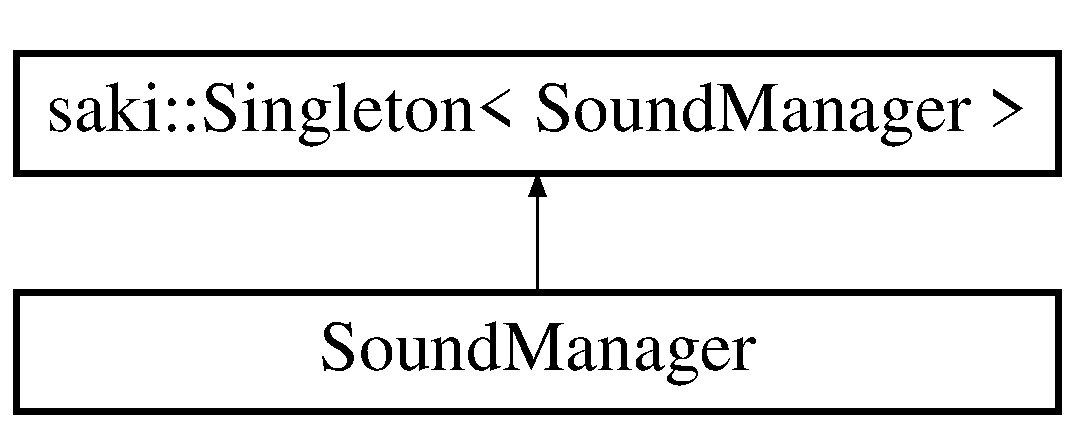
\includegraphics[height=2.000000cm]{class_sound_manager}
\end{center}
\end{figure}
\subsection*{公開メンバ関数}
\begin{DoxyCompactItemize}
\item 
std\+::unique\+\_\+ptr$<$ Direct\+X\+::\+Sound\+Effect $>$ \& \mbox{\hyperlink{class_sound_manager_a3ba4b2fe49cdc051f33aa800851f8b98}{Get\+Sound}} (W\+C\+H\+AR $\ast$)
\begin{DoxyCompactList}\small\item\em サウンドを返す \end{DoxyCompactList}\item 
void \mbox{\hyperlink{class_sound_manager_adab2bc016911756ffd973c7d781b5cfb}{Init}} (H\+W\+ND)
\begin{DoxyCompactList}\small\item\em サウンドマネージャークラスの初期化 \end{DoxyCompactList}\item 
void \mbox{\hyperlink{class_sound_manager_aaf241621221cdbefeba78e8b6bc29240}{Update}} ()
\begin{DoxyCompactList}\small\item\em サウンドマネージャーの更新 \end{DoxyCompactList}\item 
void \mbox{\hyperlink{class_sound_manager_abf0d473d0a31323c8e74684976b08e7f}{Destroy}} ()
\begin{DoxyCompactList}\small\item\em サウンドマネージャーの破棄 \end{DoxyCompactList}\item 
auto \mbox{\hyperlink{class_sound_manager_a5a575ac572eb0b50b3bb48b879a1a7e6}{Get\+Engine}} () const
\item 
void \mbox{\hyperlink{class_sound_manager_acc9fb61509f30c7eb9136386eeeb9f94}{Retry\+Audio}} ()
\item 
void \mbox{\hyperlink{class_sound_manager_a97d76cb22596fbb3c85766df0dcde757}{Suspend}} ()
\item 
void \mbox{\hyperlink{class_sound_manager_a6107940d2299131fbd7991a4f222491b}{Resume}} ()
\end{DoxyCompactItemize}
\subsection*{その他の継承メンバ}


\subsection{詳解}
サウンドを管理するクラス 

\subsection{関数詳解}
\mbox{\Hypertarget{class_sound_manager_abf0d473d0a31323c8e74684976b08e7f}\label{class_sound_manager_abf0d473d0a31323c8e74684976b08e7f}} 
\index{Sound\+Manager@{Sound\+Manager}!Destroy@{Destroy}}
\index{Destroy@{Destroy}!Sound\+Manager@{Sound\+Manager}}
\subsubsection{\texorpdfstring{Destroy()}{Destroy()}}
{\footnotesize\ttfamily void Sound\+Manager\+::\+Destroy (\begin{DoxyParamCaption}{ }\end{DoxyParamCaption})}



サウンドマネージャーの破棄 

\mbox{\Hypertarget{class_sound_manager_a5a575ac572eb0b50b3bb48b879a1a7e6}\label{class_sound_manager_a5a575ac572eb0b50b3bb48b879a1a7e6}} 
\index{Sound\+Manager@{Sound\+Manager}!Get\+Engine@{Get\+Engine}}
\index{Get\+Engine@{Get\+Engine}!Sound\+Manager@{Sound\+Manager}}
\subsubsection{\texorpdfstring{Get\+Engine()}{GetEngine()}}
{\footnotesize\ttfamily auto Sound\+Manager\+::\+Get\+Engine (\begin{DoxyParamCaption}{ }\end{DoxyParamCaption}) const\hspace{0.3cm}{\ttfamily [inline]}}

\mbox{\Hypertarget{class_sound_manager_a3ba4b2fe49cdc051f33aa800851f8b98}\label{class_sound_manager_a3ba4b2fe49cdc051f33aa800851f8b98}} 
\index{Sound\+Manager@{Sound\+Manager}!Get\+Sound@{Get\+Sound}}
\index{Get\+Sound@{Get\+Sound}!Sound\+Manager@{Sound\+Manager}}
\subsubsection{\texorpdfstring{Get\+Sound()}{GetSound()}}
{\footnotesize\ttfamily std\+::unique\+\_\+ptr$<$ Direct\+X\+::\+Sound\+Effect $>$ \& Sound\+Manager\+::\+Get\+Sound (\begin{DoxyParamCaption}\item[{W\+C\+H\+AR $\ast$}]{path }\end{DoxyParamCaption})}



サウンドを返す 


\begin{DoxyParams}{引数}
{\em path} & wavファイルのパス\\
\hline
\end{DoxyParams}
同じファイルを2度読み込まないようにする \mbox{\Hypertarget{class_sound_manager_adab2bc016911756ffd973c7d781b5cfb}\label{class_sound_manager_adab2bc016911756ffd973c7d781b5cfb}} 
\index{Sound\+Manager@{Sound\+Manager}!Init@{Init}}
\index{Init@{Init}!Sound\+Manager@{Sound\+Manager}}
\subsubsection{\texorpdfstring{Init()}{Init()}}
{\footnotesize\ttfamily void Sound\+Manager\+::\+Init (\begin{DoxyParamCaption}\item[{H\+W\+ND}]{h\+Wnd }\end{DoxyParamCaption})}



サウンドマネージャークラスの初期化 


\begin{DoxyParams}{引数}
{\em h\+Wnd} & ウィンドウハンドラ \\
\hline
\end{DoxyParams}
\mbox{\Hypertarget{class_sound_manager_a6107940d2299131fbd7991a4f222491b}\label{class_sound_manager_a6107940d2299131fbd7991a4f222491b}} 
\index{Sound\+Manager@{Sound\+Manager}!Resume@{Resume}}
\index{Resume@{Resume}!Sound\+Manager@{Sound\+Manager}}
\subsubsection{\texorpdfstring{Resume()}{Resume()}}
{\footnotesize\ttfamily void Sound\+Manager\+::\+Resume (\begin{DoxyParamCaption}{ }\end{DoxyParamCaption})\hspace{0.3cm}{\ttfamily [inline]}}

\mbox{\Hypertarget{class_sound_manager_acc9fb61509f30c7eb9136386eeeb9f94}\label{class_sound_manager_acc9fb61509f30c7eb9136386eeeb9f94}} 
\index{Sound\+Manager@{Sound\+Manager}!Retry\+Audio@{Retry\+Audio}}
\index{Retry\+Audio@{Retry\+Audio}!Sound\+Manager@{Sound\+Manager}}
\subsubsection{\texorpdfstring{Retry\+Audio()}{RetryAudio()}}
{\footnotesize\ttfamily void Sound\+Manager\+::\+Retry\+Audio (\begin{DoxyParamCaption}{ }\end{DoxyParamCaption})\hspace{0.3cm}{\ttfamily [inline]}}

\mbox{\Hypertarget{class_sound_manager_a97d76cb22596fbb3c85766df0dcde757}\label{class_sound_manager_a97d76cb22596fbb3c85766df0dcde757}} 
\index{Sound\+Manager@{Sound\+Manager}!Suspend@{Suspend}}
\index{Suspend@{Suspend}!Sound\+Manager@{Sound\+Manager}}
\subsubsection{\texorpdfstring{Suspend()}{Suspend()}}
{\footnotesize\ttfamily void Sound\+Manager\+::\+Suspend (\begin{DoxyParamCaption}{ }\end{DoxyParamCaption})\hspace{0.3cm}{\ttfamily [inline]}}

\mbox{\Hypertarget{class_sound_manager_aaf241621221cdbefeba78e8b6bc29240}\label{class_sound_manager_aaf241621221cdbefeba78e8b6bc29240}} 
\index{Sound\+Manager@{Sound\+Manager}!Update@{Update}}
\index{Update@{Update}!Sound\+Manager@{Sound\+Manager}}
\subsubsection{\texorpdfstring{Update()}{Update()}}
{\footnotesize\ttfamily void Sound\+Manager\+::\+Update (\begin{DoxyParamCaption}{ }\end{DoxyParamCaption})}



サウンドマネージャーの更新 



このクラス詳解は次のファイルから抽出されました\+:\begin{DoxyCompactItemize}
\item 
C\+:/\+Users/tokir/\+Documents/\+Git\+Hub/\+Weapon\+Merchant\+Adventure/src/sound/manager/\mbox{\hyperlink{sound__manager_8h}{sound\+\_\+manager.\+h}}\item 
C\+:/\+Users/tokir/\+Documents/\+Git\+Hub/\+Weapon\+Merchant\+Adventure/src/sound/manager/\mbox{\hyperlink{sound__manager_8cpp}{sound\+\_\+manager.\+cpp}}\end{DoxyCompactItemize}

\hypertarget{class_sprite}{}\section{Sprite クラス}
\label{class_sprite}\index{Sprite@{Sprite}}


{\ttfamily \#include $<$sprite.\+h$>$}

\subsection*{公開メンバ関数}
\begin{DoxyCompactItemize}
\item 
H\+R\+E\+S\+U\+LT \mbox{\hyperlink{class_sprite_a65b9b470731149992bfa7401ffb676ae}{Init}} (const std\+::string \&, const W\+C\+H\+AR $\ast$, \mbox{\hyperlink{common_8h_ae148fff5818e9444b4ab2288829559bf}{Vec2}} \&, const std\+::string \&=\char`\"{}shader\char`\"{}, const W\+C\+H\+AR $\ast$=L\char`\"{}sprite\+\_\+shader.\+hlsl\char`\"{}, const W\+C\+H\+AR $\ast$=L\char`\"{}sprite\+\_\+shader.\+hlsl\char`\"{}, const float=1, const float=1, const float=1, const float=1)
\item 
void \mbox{\hyperlink{class_sprite_a23296a54e3165adbbeb2b5351d04b921}{Render}} (const \mbox{\hyperlink{common_8h_a1c43cb8f0d8a41901f3ce4c67dbbce20}{Transform}} \&, const bool=true)
\item 
void \mbox{\hyperlink{class_sprite_a0a3daa8677d1205981e27bd698025afa}{Color\+Change}} (const float r, const float g, const float b, const float a)
\end{DoxyCompactItemize}
\subsection*{公開変数類}
\begin{DoxyCompactItemize}
\item 
\mbox{\hyperlink{common_8h_ae148fff5818e9444b4ab2288829559bf}{Vec2}} \mbox{\hyperlink{class_sprite_aac62c18a9b678d357f3465d45b2e6ebd}{slice\+\_\+num}}
\item 
\mbox{\hyperlink{common_8h_ae148fff5818e9444b4ab2288829559bf}{Vec2}} \mbox{\hyperlink{class_sprite_a5c96c0e7d46a79740a5fe9e71e9f132b}{prev\+\_\+slice}}
\item 
\mbox{\hyperlink{common_8h_ae148fff5818e9444b4ab2288829559bf}{Vec2}} \mbox{\hyperlink{class_sprite_a7d4903c9693bbb41094b395fe587bf47}{current\+\_\+slice}}
\item 
\mbox{\hyperlink{common_8h_ae148fff5818e9444b4ab2288829559bf}{Vec2}} \mbox{\hyperlink{class_sprite_afb8f3dc3f60aaa09306153d50e4243c9}{texture\+\_\+size}}
\item 
bool \mbox{\hyperlink{class_sprite_ae561a927089192371cff0c1b7402593b}{is\+\_\+ui\+\_\+image}} = false
\item 
float \mbox{\hyperlink{class_sprite_a4e306b23bbc378d1d973ca61084ebd9e}{percent}} = 1.\+0f
\end{DoxyCompactItemize}
\subsection*{静的公開変数類}
\begin{DoxyCompactItemize}
\item 
static int \mbox{\hyperlink{class_sprite_a9acc35b192b4150fe31b9386f7f9fc78}{depth}} = 9999
\item 
static bool \mbox{\hyperlink{class_sprite_ad4340ffd8b88519c28822eb2e9b71bf0}{has\+\_\+target}} = false
\item 
static float \mbox{\hyperlink{class_sprite_add18808500d3dca23d496757bf10259a}{target\+\_\+x}} = 0
\end{DoxyCompactItemize}


\subsection{関数詳解}
\mbox{\Hypertarget{class_sprite_a0a3daa8677d1205981e27bd698025afa}\label{class_sprite_a0a3daa8677d1205981e27bd698025afa}} 
\index{Sprite@{Sprite}!Color\+Change@{Color\+Change}}
\index{Color\+Change@{Color\+Change}!Sprite@{Sprite}}
\subsubsection{\texorpdfstring{Color\+Change()}{ColorChange()}}
{\footnotesize\ttfamily void Sprite\+::\+Color\+Change (\begin{DoxyParamCaption}\item[{const float}]{r,  }\item[{const float}]{g,  }\item[{const float}]{b,  }\item[{const float}]{a }\end{DoxyParamCaption})\hspace{0.3cm}{\ttfamily [inline]}}

\mbox{\Hypertarget{class_sprite_a65b9b470731149992bfa7401ffb676ae}\label{class_sprite_a65b9b470731149992bfa7401ffb676ae}} 
\index{Sprite@{Sprite}!Init@{Init}}
\index{Init@{Init}!Sprite@{Sprite}}
\subsubsection{\texorpdfstring{Init()}{Init()}}
{\footnotesize\ttfamily H\+R\+E\+S\+U\+LT Sprite\+::\+Init (\begin{DoxyParamCaption}\item[{const std\+::string \&}]{texture\+\_\+name,  }\item[{const W\+C\+H\+AR $\ast$}]{texture\+\_\+path,  }\item[{\mbox{\hyperlink{common_8h_ae148fff5818e9444b4ab2288829559bf}{Vec2}} \&}]{size,  }\item[{const std\+::string \&}]{shader\+\_\+name = {\ttfamily \char`\"{}shader\char`\"{}},  }\item[{const W\+C\+H\+AR $\ast$}]{v\+\_\+shader\+\_\+path = {\ttfamily L\char`\"{}sprite\+\_\+shader.hlsl\char`\"{}},  }\item[{const W\+C\+H\+AR $\ast$}]{p\+\_\+shader\+\_\+path = {\ttfamily L\char`\"{}sprite\+\_\+shader.hlsl\char`\"{}},  }\item[{const float}]{slice\+\_\+h\+\_\+num = {\ttfamily 1},  }\item[{const float}]{slice\+\_\+v\+\_\+num = {\ttfamily 1},  }\item[{const float}]{slice\+\_\+h\+\_\+init = {\ttfamily 1},  }\item[{const float}]{slice\+\_\+v\+\_\+init = {\ttfamily 1} }\end{DoxyParamCaption})}

\mbox{\Hypertarget{class_sprite_a23296a54e3165adbbeb2b5351d04b921}\label{class_sprite_a23296a54e3165adbbeb2b5351d04b921}} 
\index{Sprite@{Sprite}!Render@{Render}}
\index{Render@{Render}!Sprite@{Sprite}}
\subsubsection{\texorpdfstring{Render()}{Render()}}
{\footnotesize\ttfamily void Sprite\+::\+Render (\begin{DoxyParamCaption}\item[{const \mbox{\hyperlink{common_8h_a1c43cb8f0d8a41901f3ce4c67dbbce20}{Transform}} \&}]{transform,  }\item[{const bool}]{camera\+\_\+affected = {\ttfamily true} }\end{DoxyParamCaption})}



\subsection{メンバ詳解}
\mbox{\Hypertarget{class_sprite_a7d4903c9693bbb41094b395fe587bf47}\label{class_sprite_a7d4903c9693bbb41094b395fe587bf47}} 
\index{Sprite@{Sprite}!current\+\_\+slice@{current\+\_\+slice}}
\index{current\+\_\+slice@{current\+\_\+slice}!Sprite@{Sprite}}
\subsubsection{\texorpdfstring{current\+\_\+slice}{current\_slice}}
{\footnotesize\ttfamily \mbox{\hyperlink{common_8h_ae148fff5818e9444b4ab2288829559bf}{Vec2}} Sprite\+::current\+\_\+slice}

\mbox{\Hypertarget{class_sprite_a9acc35b192b4150fe31b9386f7f9fc78}\label{class_sprite_a9acc35b192b4150fe31b9386f7f9fc78}} 
\index{Sprite@{Sprite}!depth@{depth}}
\index{depth@{depth}!Sprite@{Sprite}}
\subsubsection{\texorpdfstring{depth}{depth}}
{\footnotesize\ttfamily int Sprite\+::depth = 9999\hspace{0.3cm}{\ttfamily [static]}}

\mbox{\Hypertarget{class_sprite_ad4340ffd8b88519c28822eb2e9b71bf0}\label{class_sprite_ad4340ffd8b88519c28822eb2e9b71bf0}} 
\index{Sprite@{Sprite}!has\+\_\+target@{has\+\_\+target}}
\index{has\+\_\+target@{has\+\_\+target}!Sprite@{Sprite}}
\subsubsection{\texorpdfstring{has\+\_\+target}{has\_target}}
{\footnotesize\ttfamily bool Sprite\+::has\+\_\+target = false\hspace{0.3cm}{\ttfamily [static]}}

\mbox{\Hypertarget{class_sprite_ae561a927089192371cff0c1b7402593b}\label{class_sprite_ae561a927089192371cff0c1b7402593b}} 
\index{Sprite@{Sprite}!is\+\_\+ui\+\_\+image@{is\+\_\+ui\+\_\+image}}
\index{is\+\_\+ui\+\_\+image@{is\+\_\+ui\+\_\+image}!Sprite@{Sprite}}
\subsubsection{\texorpdfstring{is\+\_\+ui\+\_\+image}{is\_ui\_image}}
{\footnotesize\ttfamily bool Sprite\+::is\+\_\+ui\+\_\+image = false}

\mbox{\Hypertarget{class_sprite_a4e306b23bbc378d1d973ca61084ebd9e}\label{class_sprite_a4e306b23bbc378d1d973ca61084ebd9e}} 
\index{Sprite@{Sprite}!percent@{percent}}
\index{percent@{percent}!Sprite@{Sprite}}
\subsubsection{\texorpdfstring{percent}{percent}}
{\footnotesize\ttfamily float Sprite\+::percent = 1.\+0f}

\mbox{\Hypertarget{class_sprite_a5c96c0e7d46a79740a5fe9e71e9f132b}\label{class_sprite_a5c96c0e7d46a79740a5fe9e71e9f132b}} 
\index{Sprite@{Sprite}!prev\+\_\+slice@{prev\+\_\+slice}}
\index{prev\+\_\+slice@{prev\+\_\+slice}!Sprite@{Sprite}}
\subsubsection{\texorpdfstring{prev\+\_\+slice}{prev\_slice}}
{\footnotesize\ttfamily \mbox{\hyperlink{common_8h_ae148fff5818e9444b4ab2288829559bf}{Vec2}} Sprite\+::prev\+\_\+slice}

\mbox{\Hypertarget{class_sprite_aac62c18a9b678d357f3465d45b2e6ebd}\label{class_sprite_aac62c18a9b678d357f3465d45b2e6ebd}} 
\index{Sprite@{Sprite}!slice\+\_\+num@{slice\+\_\+num}}
\index{slice\+\_\+num@{slice\+\_\+num}!Sprite@{Sprite}}
\subsubsection{\texorpdfstring{slice\+\_\+num}{slice\_num}}
{\footnotesize\ttfamily \mbox{\hyperlink{common_8h_ae148fff5818e9444b4ab2288829559bf}{Vec2}} Sprite\+::slice\+\_\+num}

\mbox{\Hypertarget{class_sprite_add18808500d3dca23d496757bf10259a}\label{class_sprite_add18808500d3dca23d496757bf10259a}} 
\index{Sprite@{Sprite}!target\+\_\+x@{target\+\_\+x}}
\index{target\+\_\+x@{target\+\_\+x}!Sprite@{Sprite}}
\subsubsection{\texorpdfstring{target\+\_\+x}{target\_x}}
{\footnotesize\ttfamily float Sprite\+::target\+\_\+x = 0\hspace{0.3cm}{\ttfamily [static]}}

\mbox{\Hypertarget{class_sprite_afb8f3dc3f60aaa09306153d50e4243c9}\label{class_sprite_afb8f3dc3f60aaa09306153d50e4243c9}} 
\index{Sprite@{Sprite}!texture\+\_\+size@{texture\+\_\+size}}
\index{texture\+\_\+size@{texture\+\_\+size}!Sprite@{Sprite}}
\subsubsection{\texorpdfstring{texture\+\_\+size}{texture\_size}}
{\footnotesize\ttfamily \mbox{\hyperlink{common_8h_ae148fff5818e9444b4ab2288829559bf}{Vec2}} Sprite\+::texture\+\_\+size}



このクラス詳解は次のファイルから抽出されました\+:\begin{DoxyCompactItemize}
\item 
C\+:/\+Users/tokir/\+Documents/\+Git\+Hub/\+Weapon\+Merchant\+Adventure/src/src/sprite/\mbox{\hyperlink{sprite_8h}{sprite.\+h}}\item 
C\+:/\+Users/tokir/\+Documents/\+Git\+Hub/\+Weapon\+Merchant\+Adventure/src/src/sprite/\mbox{\hyperlink{sprite_8cpp}{sprite.\+cpp}}\end{DoxyCompactItemize}

\hypertarget{class_sprite_manager}{}\section{Sprite\+Manager クラス}
\label{class_sprite_manager}\index{Sprite\+Manager@{Sprite\+Manager}}


Sprite関係のデバイスや描画時に経由するものを管理するクラス  




{\ttfamily \#include $<$sprite\+\_\+manager.\+h$>$}

Sprite\+Manager の継承関係図\begin{figure}[H]
\begin{center}
\leavevmode
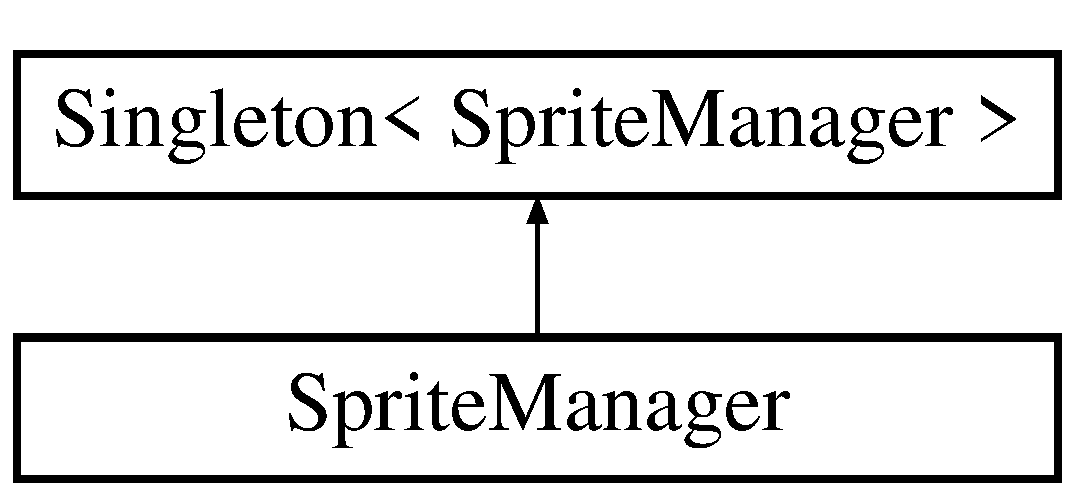
\includegraphics[height=2.000000cm]{class_sprite_manager}
\end{center}
\end{figure}
\subsection*{公開メンバ関数}
\begin{DoxyCompactItemize}
\item 
void \mbox{\hyperlink{class_sprite_manager_a82941ce284548c762f250220ea58f43c}{Init}} ()
\begin{DoxyCompactList}\small\item\em 初期化 \end{DoxyCompactList}\item 
void \mbox{\hyperlink{class_sprite_manager_a5b41702bb7476fb1c148b3e2c81d6b06}{Set\+Texture}} (std\+::string, W\+C\+H\+AR $\ast$)
\begin{DoxyCompactList}\small\item\em テクスチャを保存 \end{DoxyCompactList}\item 
void \mbox{\hyperlink{class_sprite_manager_a4cdd5540bace32d5742ea4df648d87e9}{Render}} (const \mbox{\hyperlink{class_transform}{Transform}} \&, bool, bool, const std\+::string \&, const Direct\+X\+::\+X\+M\+V\+E\+C\+T\+OR \&, const R\+E\+CT \&, const Direct\+X\+::\+Sprite\+Effects)
\begin{DoxyCompactList}\small\item\em 描画 \end{DoxyCompactList}\item 
\mbox{\hyperlink{class_sprite_manager_ae01a31b1c80f676604ba55c93b499e1f}{$\sim$\+Sprite\+Manager}} ()
\begin{DoxyCompactList}\small\item\em デストラクタ \end{DoxyCompactList}\item 
std\+::unique\+\_\+ptr$<$ Direct\+X\+::\+Sprite\+Batch $>$ \& \mbox{\hyperlink{class_sprite_manager_a0b82bacf33d0b558657c8e9841daf9d9}{Get\+Sprite\+Batch}} ()
\begin{DoxyCompactList}\small\item\em Sprite\+Batchのゲッタ \end{DoxyCompactList}\item 
I\+D3\+D11\+Device $\ast$\& \mbox{\hyperlink{class_sprite_manager_ac9e2c44cc43775d9802612bd4be9bac3}{Get\+Device}} ()
\begin{DoxyCompactList}\small\item\em I\+D3\+D11\+Deviceのゲッタ \end{DoxyCompactList}\item 
I\+D3\+D11\+Device\+Context $\ast$\& \mbox{\hyperlink{class_sprite_manager_a6bad23e380818dbe6b521adc07ab84fa}{Get\+Device\+Context}} ()
\begin{DoxyCompactList}\small\item\em I\+D3\+D11\+Device\+Contextのゲッタ \end{DoxyCompactList}\item 
void \mbox{\hyperlink{class_sprite_manager_a6b387e8736713264f6d590082cd492cb}{Start}} ()
\begin{DoxyCompactList}\small\item\em 描画をスタート \end{DoxyCompactList}\item 
void \mbox{\hyperlink{class_sprite_manager_afed8a96a6530f67123a4efa1b6d77032}{End}} ()
\begin{DoxyCompactList}\small\item\em 描画を終了 \end{DoxyCompactList}\end{DoxyCompactItemize}
\subsection*{その他の継承メンバ}


\subsection{詳解}
Sprite関係のデバイスや描画時に経由するものを管理するクラス 

\subsection{構築子と解体子}
\mbox{\Hypertarget{class_sprite_manager_ae01a31b1c80f676604ba55c93b499e1f}\label{class_sprite_manager_ae01a31b1c80f676604ba55c93b499e1f}} 
\index{Sprite\+Manager@{Sprite\+Manager}!````~Sprite\+Manager@{$\sim$\+Sprite\+Manager}}
\index{````~Sprite\+Manager@{$\sim$\+Sprite\+Manager}!Sprite\+Manager@{Sprite\+Manager}}
\subsubsection{\texorpdfstring{$\sim$\+Sprite\+Manager()}{~SpriteManager()}}
{\footnotesize\ttfamily Sprite\+Manager\+::$\sim$\+Sprite\+Manager (\begin{DoxyParamCaption}{ }\end{DoxyParamCaption})}



デストラクタ 



\subsection{関数詳解}
\mbox{\Hypertarget{class_sprite_manager_afed8a96a6530f67123a4efa1b6d77032}\label{class_sprite_manager_afed8a96a6530f67123a4efa1b6d77032}} 
\index{Sprite\+Manager@{Sprite\+Manager}!End@{End}}
\index{End@{End}!Sprite\+Manager@{Sprite\+Manager}}
\subsubsection{\texorpdfstring{End()}{End()}}
{\footnotesize\ttfamily void Sprite\+Manager\+::\+End (\begin{DoxyParamCaption}{ }\end{DoxyParamCaption})\hspace{0.3cm}{\ttfamily [inline]}}



描画を終了 

\mbox{\Hypertarget{class_sprite_manager_ac9e2c44cc43775d9802612bd4be9bac3}\label{class_sprite_manager_ac9e2c44cc43775d9802612bd4be9bac3}} 
\index{Sprite\+Manager@{Sprite\+Manager}!Get\+Device@{Get\+Device}}
\index{Get\+Device@{Get\+Device}!Sprite\+Manager@{Sprite\+Manager}}
\subsubsection{\texorpdfstring{Get\+Device()}{GetDevice()}}
{\footnotesize\ttfamily I\+D3\+D11\+Device$\ast$\& Sprite\+Manager\+::\+Get\+Device (\begin{DoxyParamCaption}{ }\end{DoxyParamCaption})\hspace{0.3cm}{\ttfamily [inline]}}



I\+D3\+D11\+Deviceのゲッタ 

\begin{DoxyReturn}{戻り値}
I\+D3\+D11\+Device$\ast$\& 
\end{DoxyReturn}
\mbox{\Hypertarget{class_sprite_manager_a6bad23e380818dbe6b521adc07ab84fa}\label{class_sprite_manager_a6bad23e380818dbe6b521adc07ab84fa}} 
\index{Sprite\+Manager@{Sprite\+Manager}!Get\+Device\+Context@{Get\+Device\+Context}}
\index{Get\+Device\+Context@{Get\+Device\+Context}!Sprite\+Manager@{Sprite\+Manager}}
\subsubsection{\texorpdfstring{Get\+Device\+Context()}{GetDeviceContext()}}
{\footnotesize\ttfamily I\+D3\+D11\+Device\+Context$\ast$\& Sprite\+Manager\+::\+Get\+Device\+Context (\begin{DoxyParamCaption}{ }\end{DoxyParamCaption})\hspace{0.3cm}{\ttfamily [inline]}}



I\+D3\+D11\+Device\+Contextのゲッタ 

\begin{DoxyReturn}{戻り値}
I\+D3\+D11\+Device\+Context$\ast$\& 
\end{DoxyReturn}
\mbox{\Hypertarget{class_sprite_manager_a0b82bacf33d0b558657c8e9841daf9d9}\label{class_sprite_manager_a0b82bacf33d0b558657c8e9841daf9d9}} 
\index{Sprite\+Manager@{Sprite\+Manager}!Get\+Sprite\+Batch@{Get\+Sprite\+Batch}}
\index{Get\+Sprite\+Batch@{Get\+Sprite\+Batch}!Sprite\+Manager@{Sprite\+Manager}}
\subsubsection{\texorpdfstring{Get\+Sprite\+Batch()}{GetSpriteBatch()}}
{\footnotesize\ttfamily std\+::unique\+\_\+ptr$<$Direct\+X\+::\+Sprite\+Batch$>$\& Sprite\+Manager\+::\+Get\+Sprite\+Batch (\begin{DoxyParamCaption}{ }\end{DoxyParamCaption})\hspace{0.3cm}{\ttfamily [inline]}}



Sprite\+Batchのゲッタ 

\begin{DoxyReturn}{戻り値}
std\+::unique\+\_\+ptr$<$\+Direct\+X\+::\+Sprite\+Batch$>$\& 
\end{DoxyReturn}
\mbox{\Hypertarget{class_sprite_manager_a82941ce284548c762f250220ea58f43c}\label{class_sprite_manager_a82941ce284548c762f250220ea58f43c}} 
\index{Sprite\+Manager@{Sprite\+Manager}!Init@{Init}}
\index{Init@{Init}!Sprite\+Manager@{Sprite\+Manager}}
\subsubsection{\texorpdfstring{Init()}{Init()}}
{\footnotesize\ttfamily void Sprite\+Manager\+::\+Init (\begin{DoxyParamCaption}{ }\end{DoxyParamCaption})}



初期化 

\mbox{\Hypertarget{class_sprite_manager_a4cdd5540bace32d5742ea4df648d87e9}\label{class_sprite_manager_a4cdd5540bace32d5742ea4df648d87e9}} 
\index{Sprite\+Manager@{Sprite\+Manager}!Render@{Render}}
\index{Render@{Render}!Sprite\+Manager@{Sprite\+Manager}}
\subsubsection{\texorpdfstring{Render()}{Render()}}
{\footnotesize\ttfamily void Sprite\+Manager\+::\+Render (\begin{DoxyParamCaption}\item[{const \mbox{\hyperlink{class_transform}{Transform}} \&}]{transform,  }\item[{bool}]{affected\+\_\+camera,  }\item[{bool}]{center\+\_\+axis,  }\item[{const std\+::string \&}]{name,  }\item[{const Direct\+X\+::\+X\+M\+V\+E\+C\+T\+OR \&}]{color,  }\item[{const R\+E\+CT \&}]{rect,  }\item[{const Direct\+X\+::\+Sprite\+Effects}]{sprite\+\_\+effect }\end{DoxyParamCaption})}



描画 


\begin{DoxyParams}{引数}
{\em transform} & 位置や回転、拡大・縮小等 \\
\hline
{\em affected\+\_\+camera} & カメラの影響を受けるかどうか \\
\hline
{\em center\+\_\+axis} & センターを軸にするかどうか \\
\hline
{\em name} & キー \\
\hline
{\em color} & 色 \\
\hline
{\em rect} & テクスチャのどこを描画するかどうか \\
\hline
{\em sprite\+\_\+effect} & 様々の方向の反転 \\
\hline
\end{DoxyParams}
\mbox{\Hypertarget{class_sprite_manager_a5b41702bb7476fb1c148b3e2c81d6b06}\label{class_sprite_manager_a5b41702bb7476fb1c148b3e2c81d6b06}} 
\index{Sprite\+Manager@{Sprite\+Manager}!Set\+Texture@{Set\+Texture}}
\index{Set\+Texture@{Set\+Texture}!Sprite\+Manager@{Sprite\+Manager}}
\subsubsection{\texorpdfstring{Set\+Texture()}{SetTexture()}}
{\footnotesize\ttfamily void Sprite\+Manager\+::\+Set\+Texture (\begin{DoxyParamCaption}\item[{std\+::string}]{name,  }\item[{W\+C\+H\+AR $\ast$}]{path }\end{DoxyParamCaption})}



テクスチャを保存 


\begin{DoxyParams}{引数}
{\em name} & mapで管理するためのキー \\
\hline
{\em path} & テクスチャがあるパス \\
\hline
\end{DoxyParams}
\mbox{\Hypertarget{class_sprite_manager_a6b387e8736713264f6d590082cd492cb}\label{class_sprite_manager_a6b387e8736713264f6d590082cd492cb}} 
\index{Sprite\+Manager@{Sprite\+Manager}!Start@{Start}}
\index{Start@{Start}!Sprite\+Manager@{Sprite\+Manager}}
\subsubsection{\texorpdfstring{Start()}{Start()}}
{\footnotesize\ttfamily void Sprite\+Manager\+::\+Start (\begin{DoxyParamCaption}{ }\end{DoxyParamCaption})\hspace{0.3cm}{\ttfamily [inline]}}



描画をスタート 



このクラス詳解は次のファイルから抽出されました\+:\begin{DoxyCompactItemize}
\item 
C\+:/\+Users/tokir/\+Documents/\+Git\+Hub/\+Weapon\+Merchant\+Adventure/src/rendering/sprite/manager/\mbox{\hyperlink{sprite__manager_8h}{sprite\+\_\+manager.\+h}}\item 
C\+:/\+Users/tokir/\+Documents/\+Git\+Hub/\+Weapon\+Merchant\+Adventure/src/rendering/sprite/manager/\mbox{\hyperlink{sprite__manager_8cpp}{sprite\+\_\+manager.\+cpp}}\end{DoxyCompactItemize}

\hypertarget{class_title_scene}{}\section{Title\+Scene クラス}
\label{class_title_scene}\index{Title\+Scene@{Title\+Scene}}


タイトルシーンクラス  




{\ttfamily \#include $<$title\+\_\+scene.\+h$>$}

Title\+Scene の継承関係図\begin{figure}[H]
\begin{center}
\leavevmode
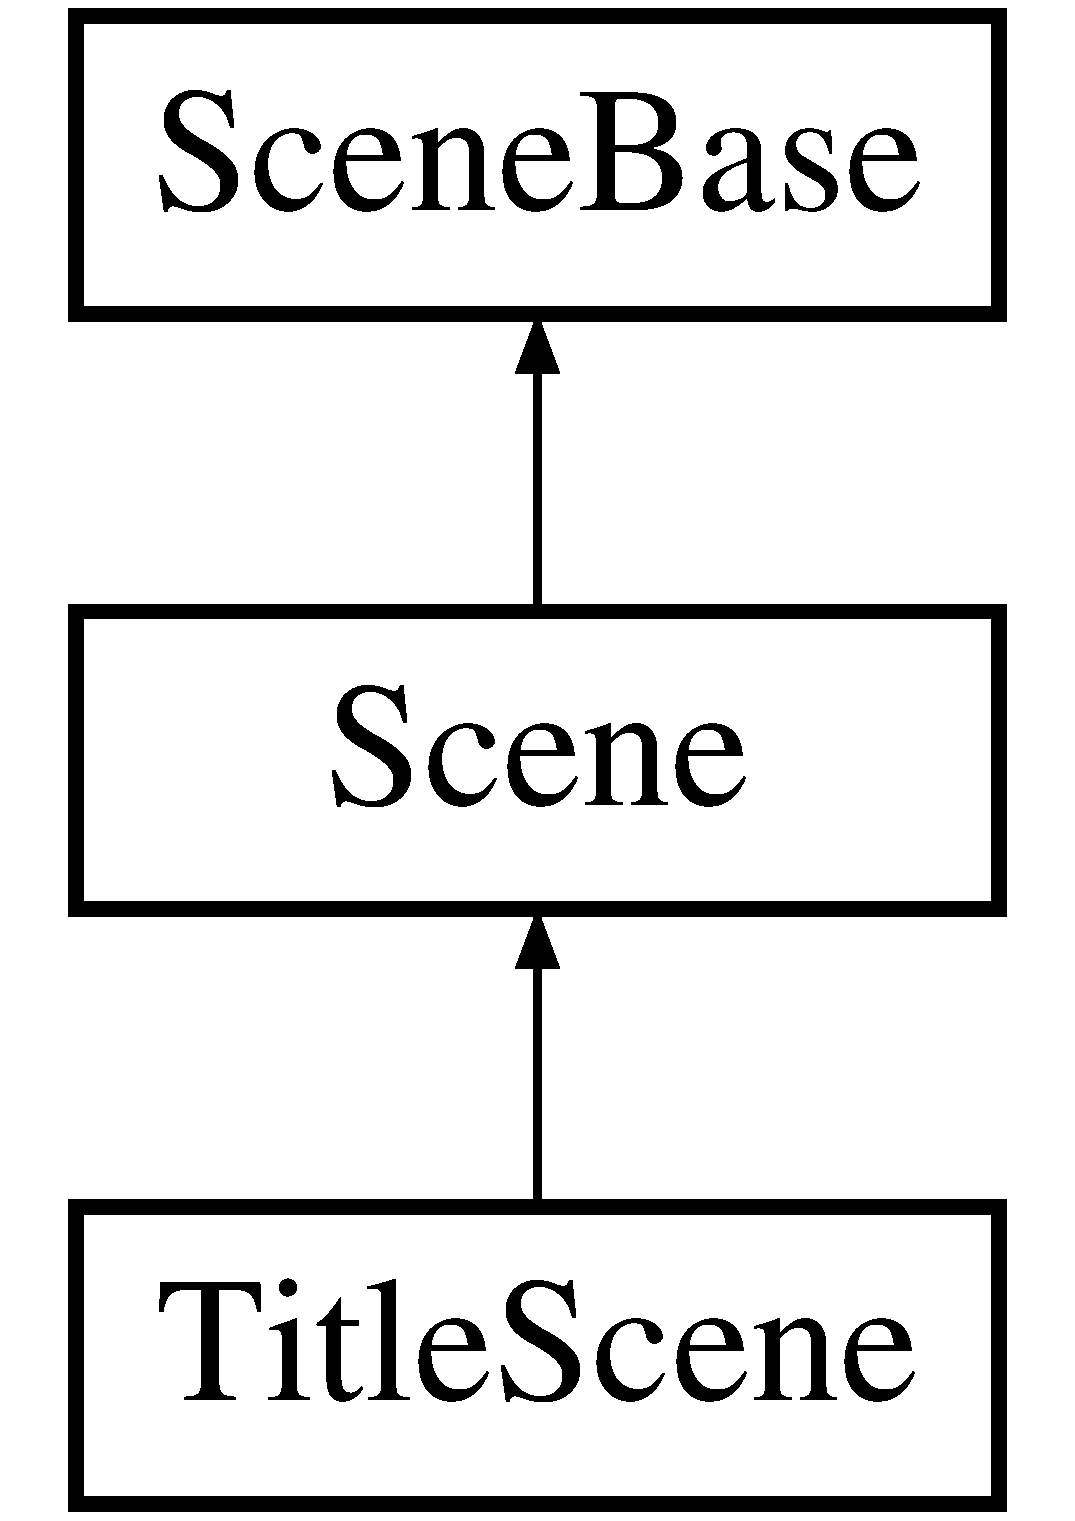
\includegraphics[height=3.000000cm]{class_title_scene}
\end{center}
\end{figure}
\subsection*{公開メンバ関数}
\begin{DoxyCompactItemize}
\item 
void \mbox{\hyperlink{class_title_scene_a3d039e7db0fa1e22e8c36d3cedfbd318}{Init}} () final
\begin{DoxyCompactList}\small\item\em タイトルシーンの初期化 \end{DoxyCompactList}\item 
\mbox{\hyperlink{scene__base_8h_a24cee5343fb9d0706ead6e8601f363be}{S\+C\+E\+NE}} \mbox{\hyperlink{class_title_scene_a19f6ee49ca6c8526fb1af2c0a2df9a33}{Update}} () final
\begin{DoxyCompactList}\small\item\em タイトルシーンの更新 \end{DoxyCompactList}\item 
void \mbox{\hyperlink{class_title_scene_af12c59b3bf9458640938c5ca620527ae}{Render}} () final
\begin{DoxyCompactList}\small\item\em タイトルシーンの描画 \end{DoxyCompactList}\item 
void \mbox{\hyperlink{class_title_scene_adfbc5f934572ede2e36419b089c88fe8}{Destroy}} () final
\begin{DoxyCompactList}\small\item\em タイトルシーンの破棄 \end{DoxyCompactList}\end{DoxyCompactItemize}
\subsection*{その他の継承メンバ}


\subsection{詳解}
タイトルシーンクラス 

\subsection{関数詳解}
\mbox{\Hypertarget{class_title_scene_adfbc5f934572ede2e36419b089c88fe8}\label{class_title_scene_adfbc5f934572ede2e36419b089c88fe8}} 
\index{Title\+Scene@{Title\+Scene}!Destroy@{Destroy}}
\index{Destroy@{Destroy}!Title\+Scene@{Title\+Scene}}
\subsubsection{\texorpdfstring{Destroy()}{Destroy()}}
{\footnotesize\ttfamily void Title\+Scene\+::\+Destroy (\begin{DoxyParamCaption}{ }\end{DoxyParamCaption})\hspace{0.3cm}{\ttfamily [final]}, {\ttfamily [virtual]}}



タイトルシーンの破棄 



\mbox{\hyperlink{class_scene_base_a7c5b54020bc519b4dadfe9770d6b27f7}{Scene\+Base}}を実装しています。

\mbox{\Hypertarget{class_title_scene_a3d039e7db0fa1e22e8c36d3cedfbd318}\label{class_title_scene_a3d039e7db0fa1e22e8c36d3cedfbd318}} 
\index{Title\+Scene@{Title\+Scene}!Init@{Init}}
\index{Init@{Init}!Title\+Scene@{Title\+Scene}}
\subsubsection{\texorpdfstring{Init()}{Init()}}
{\footnotesize\ttfamily void Title\+Scene\+::\+Init (\begin{DoxyParamCaption}{ }\end{DoxyParamCaption})\hspace{0.3cm}{\ttfamily [final]}, {\ttfamily [virtual]}}



タイトルシーンの初期化 



\mbox{\hyperlink{class_scene_base_a24d7db43c819924dc8b07b436f6d3148}{Scene\+Base}}を実装しています。

\mbox{\Hypertarget{class_title_scene_af12c59b3bf9458640938c5ca620527ae}\label{class_title_scene_af12c59b3bf9458640938c5ca620527ae}} 
\index{Title\+Scene@{Title\+Scene}!Render@{Render}}
\index{Render@{Render}!Title\+Scene@{Title\+Scene}}
\subsubsection{\texorpdfstring{Render()}{Render()}}
{\footnotesize\ttfamily void Title\+Scene\+::\+Render (\begin{DoxyParamCaption}{ }\end{DoxyParamCaption})\hspace{0.3cm}{\ttfamily [final]}, {\ttfamily [virtual]}}



タイトルシーンの描画 



\mbox{\hyperlink{class_scene_base_ad981674ce731ea267f398e889bbb9dc3}{Scene\+Base}}を実装しています。

\mbox{\Hypertarget{class_title_scene_a19f6ee49ca6c8526fb1af2c0a2df9a33}\label{class_title_scene_a19f6ee49ca6c8526fb1af2c0a2df9a33}} 
\index{Title\+Scene@{Title\+Scene}!Update@{Update}}
\index{Update@{Update}!Title\+Scene@{Title\+Scene}}
\subsubsection{\texorpdfstring{Update()}{Update()}}
{\footnotesize\ttfamily \mbox{\hyperlink{scene__base_8h_a24cee5343fb9d0706ead6e8601f363be}{S\+C\+E\+NE}} Title\+Scene\+::\+Update (\begin{DoxyParamCaption}{ }\end{DoxyParamCaption})\hspace{0.3cm}{\ttfamily [final]}, {\ttfamily [virtual]}}



タイトルシーンの更新 

\begin{DoxyReturn}{戻り値}
S\+C\+E\+NE シーンが変わるなら次のシーンのenum classを返す 
\end{DoxyReturn}


\mbox{\hyperlink{class_scene_acb50f8104e5a7cfecbdececa7d5f1b39}{Scene}}を実装しています。



このクラス詳解は次のファイルから抽出されました\+:\begin{DoxyCompactItemize}
\item 
C\+:/\+Users/tokir/\+Documents/\+Git\+Hub/\+Weapon\+Merchant\+Adventure/src/scene/main/title/\mbox{\hyperlink{title__scene_8h}{title\+\_\+scene.\+h}}\item 
C\+:/\+Users/tokir/\+Documents/\+Git\+Hub/\+Weapon\+Merchant\+Adventure/src/scene/main/title/\mbox{\hyperlink{title__scene_8cpp}{title\+\_\+scene.\+cpp}}\end{DoxyCompactItemize}

\hypertarget{class_transform}{}\section{Transform クラス}
\label{class_transform}\index{Transform@{Transform}}


{\ttfamily \#include $<$transform.\+h$>$}

\subsection*{公開メンバ関数}
\begin{DoxyCompactItemize}
\item 
\mbox{\hyperlink{class_transform_aa08ca4266efabc768973cdeea51945ab}{Transform}} ()
\item 
\mbox{\hyperlink{class_transform_afdda2868df3ca6b122c5e52f7919a692}{Transform}} (const float, const float=0, const float=0, const float=1)
\begin{DoxyCompactList}\small\item\em posをそれぞれのパラメータで受け取るコンストラクタ \end{DoxyCompactList}\item 
\mbox{\hyperlink{class_transform_aae9fd575f9e6e4862ea2d9232340e6dd}{Transform}} (const \mbox{\hyperlink{transform_8h_afb0c5e21d4133ff4f200992c0b534e1b}{V\+E\+C2}} \&\+\_\+pos, const float \+\_\+rot, const float \+\_\+scale)
\begin{DoxyCompactList}\small\item\em posを\+V\+E\+C2クラスで受け取るコンストラクタ \end{DoxyCompactList}\item 
\mbox{\hyperlink{class_transform_a7790f3c5dfe2b7fe7997af5f23e2ec7d}{Transform}} (const \mbox{\hyperlink{class_transform}{Transform}} \&t)
\begin{DoxyCompactList}\small\item\em コピーコンストラクタ \end{DoxyCompactList}\item 
void \mbox{\hyperlink{class_transform_a39816379bc1e3a0bbae23fa94db576f1}{Init}} (const float, const float=0, const float=0, const float=1)
\begin{DoxyCompactList}\small\item\em 一つ一つ値で渡す初期化 \end{DoxyCompactList}\item 
void \mbox{\hyperlink{class_transform_a0ccfc45e47071b7ebed1a61a14a202c4}{Init}} (const \mbox{\hyperlink{transform_8h_afb0c5e21d4133ff4f200992c0b534e1b}{V\+E\+C2}} \&\+\_\+pos, const float \+\_\+rot, const float \+\_\+scale)
\begin{DoxyCompactList}\small\item\em 各クラスに対して値を渡す初期化 \end{DoxyCompactList}\item 
void \mbox{\hyperlink{class_transform_a2d0cb73aca3f73de81f2bf8463cdb942}{Init}} (const \mbox{\hyperlink{class_transform}{Transform}} \&t)
\begin{DoxyCompactList}\small\item\em Transformクラスを渡す初期化 \end{DoxyCompactList}\item 
void \mbox{\hyperlink{class_transform_a45772ecb47b60d5b3f110613c3f15984}{Move}} (const float, const float)
\begin{DoxyCompactList}\small\item\em 一つ一つ値で渡す移動 \end{DoxyCompactList}\item 
void \mbox{\hyperlink{class_transform_a13dbb800ca989856d1f56c03dd9a0ad0}{Move}} (const \mbox{\hyperlink{transform_8h_afb0c5e21d4133ff4f200992c0b534e1b}{V\+E\+C2}} \&)
\begin{DoxyCompactList}\small\item\em  クラスで渡す移動 \end{DoxyCompactList}\item 
void \mbox{\hyperlink{class_transform_a696d7e837eafa09409150fb055daa223}{Rotate}} (const float)
\begin{DoxyCompactList}\small\item\em  回転 \end{DoxyCompactList}\item 
void \mbox{\hyperlink{class_transform_ad6097ddf1d30f5a1023725efbee375fb}{Scaling}} (const float)
\begin{DoxyCompactList}\small\item\em  拡大・縮小 \end{DoxyCompactList}\item 
void \mbox{\hyperlink{class_transform_af1a25489903986022218a798e4f40251}{operator=}} (const \mbox{\hyperlink{class_transform}{Transform}} \&)
\item 
void \mbox{\hyperlink{class_transform_a3b0aa54a1ca373ec3a7052977b5bf826}{operator+=}} (const \mbox{\hyperlink{class_transform}{Transform}} \&)
\item 
void \mbox{\hyperlink{class_transform_a204ee3471c1d08188076e3645c9f3517}{operator-\/=}} (const \mbox{\hyperlink{class_transform}{Transform}} \&)
\item 
void \mbox{\hyperlink{class_transform_a3746d6759ca289e8cd4982e889e7ec6b}{operator$\ast$=}} (const \mbox{\hyperlink{class_transform}{Transform}} \&)
\item 
void \mbox{\hyperlink{class_transform_ab13378f63abf5bc132841f83423a634d}{operator$\ast$=}} (const float)
\item 
void \mbox{\hyperlink{class_transform_aa38455bbe5aed5f9dfd98a8d3b8a24ec}{operator/=}} (const float)
\item 
\mbox{\hyperlink{class_transform}{Transform}} \mbox{\hyperlink{class_transform_a8e21c258146adde8ca798878bab9ce9d}{operator+}} (const \mbox{\hyperlink{class_transform}{Transform}} \&) const
\item 
\mbox{\hyperlink{class_transform}{Transform}} \mbox{\hyperlink{class_transform_a17493155309aa1650de99ce384f096a6}{operator-\/}} (const \mbox{\hyperlink{class_transform}{Transform}} \&) const
\item 
bool \mbox{\hyperlink{class_transform_a0a2d49f8c1b9a2229846534f9bcc63d4}{operator==}} (const \mbox{\hyperlink{class_transform}{Transform}} \&) const
\item 
bool \mbox{\hyperlink{class_transform_ae0aed78dcd6aaeb786ec0bdadafa9498}{operator!=}} (const \mbox{\hyperlink{class_transform}{Transform}} \&) const
\end{DoxyCompactItemize}
\subsection*{公開変数類}
\begin{DoxyCompactItemize}
\item 
\mbox{\hyperlink{transform_8h_afb0c5e21d4133ff4f200992c0b534e1b}{V\+E\+C2}} \mbox{\hyperlink{class_transform_a25bce2389cc280e8adf193bdbb00d94a}{pos}}
\item 
float \mbox{\hyperlink{class_transform_a2b471ae0000c6959dc9b07263933aa43}{rot}}
\item 
float \mbox{\hyperlink{class_transform_a631712eb230305f58d164086d492701b}{scale}}
\item 
\mbox{\hyperlink{transform_8h_afb0c5e21d4133ff4f200992c0b534e1b}{V\+E\+C2}} \mbox{\hyperlink{class_transform_a83e0bdbf8a2b4a45197d17d7415a6874}{size}}
\end{DoxyCompactItemize}


\subsection{詳解}
クラス 

\subsection{構築子と解体子}
\mbox{\Hypertarget{class_transform_aa08ca4266efabc768973cdeea51945ab}\label{class_transform_aa08ca4266efabc768973cdeea51945ab}} 
\index{Transform@{Transform}!Transform@{Transform}}
\index{Transform@{Transform}!Transform@{Transform}}
\subsubsection{\texorpdfstring{Transform()}{Transform()}\hspace{0.1cm}{\footnotesize\ttfamily [1/4]}}
{\footnotesize\ttfamily Transform\+::\+Transform (\begin{DoxyParamCaption}{ }\end{DoxyParamCaption})}

\+:brief ゼロで初期化する引数なしコンストラクタ \mbox{\Hypertarget{class_transform_afdda2868df3ca6b122c5e52f7919a692}\label{class_transform_afdda2868df3ca6b122c5e52f7919a692}} 
\index{Transform@{Transform}!Transform@{Transform}}
\index{Transform@{Transform}!Transform@{Transform}}
\subsubsection{\texorpdfstring{Transform()}{Transform()}\hspace{0.1cm}{\footnotesize\ttfamily [2/4]}}
{\footnotesize\ttfamily Transform\+::\+Transform (\begin{DoxyParamCaption}\item[{const float}]{posx,  }\item[{const float}]{posy = {\ttfamily 0},  }\item[{const float}]{\+\_\+rot = {\ttfamily 0},  }\item[{const float}]{\+\_\+scale = {\ttfamily 1} }\end{DoxyParamCaption})}



posをそれぞれのパラメータで受け取るコンストラクタ 

\mbox{\Hypertarget{class_transform_aae9fd575f9e6e4862ea2d9232340e6dd}\label{class_transform_aae9fd575f9e6e4862ea2d9232340e6dd}} 
\index{Transform@{Transform}!Transform@{Transform}}
\index{Transform@{Transform}!Transform@{Transform}}
\subsubsection{\texorpdfstring{Transform()}{Transform()}\hspace{0.1cm}{\footnotesize\ttfamily [3/4]}}
{\footnotesize\ttfamily Transform\+::\+Transform (\begin{DoxyParamCaption}\item[{const \mbox{\hyperlink{transform_8h_afb0c5e21d4133ff4f200992c0b534e1b}{V\+E\+C2}} \&}]{\+\_\+pos,  }\item[{const float}]{\+\_\+rot,  }\item[{const float}]{\+\_\+scale }\end{DoxyParamCaption})}



posを\+V\+E\+C2クラスで受け取るコンストラクタ 

\mbox{\Hypertarget{class_transform_a7790f3c5dfe2b7fe7997af5f23e2ec7d}\label{class_transform_a7790f3c5dfe2b7fe7997af5f23e2ec7d}} 
\index{Transform@{Transform}!Transform@{Transform}}
\index{Transform@{Transform}!Transform@{Transform}}
\subsubsection{\texorpdfstring{Transform()}{Transform()}\hspace{0.1cm}{\footnotesize\ttfamily [4/4]}}
{\footnotesize\ttfamily Transform\+::\+Transform (\begin{DoxyParamCaption}\item[{const \mbox{\hyperlink{class_transform}{Transform}} \&}]{t }\end{DoxyParamCaption})}



コピーコンストラクタ 



\subsection{関数詳解}
\mbox{\Hypertarget{class_transform_a39816379bc1e3a0bbae23fa94db576f1}\label{class_transform_a39816379bc1e3a0bbae23fa94db576f1}} 
\index{Transform@{Transform}!Init@{Init}}
\index{Init@{Init}!Transform@{Transform}}
\subsubsection{\texorpdfstring{Init()}{Init()}\hspace{0.1cm}{\footnotesize\ttfamily [1/3]}}
{\footnotesize\ttfamily void Transform\+::\+Init (\begin{DoxyParamCaption}\item[{const float}]{posx,  }\item[{const float}]{posy = {\ttfamily 0},  }\item[{const float}]{\+\_\+rot = {\ttfamily 0},  }\item[{const float}]{\+\_\+scale = {\ttfamily 1} }\end{DoxyParamCaption})}



一つ一つ値で渡す初期化 

\mbox{\Hypertarget{class_transform_a0ccfc45e47071b7ebed1a61a14a202c4}\label{class_transform_a0ccfc45e47071b7ebed1a61a14a202c4}} 
\index{Transform@{Transform}!Init@{Init}}
\index{Init@{Init}!Transform@{Transform}}
\subsubsection{\texorpdfstring{Init()}{Init()}\hspace{0.1cm}{\footnotesize\ttfamily [2/3]}}
{\footnotesize\ttfamily void Transform\+::\+Init (\begin{DoxyParamCaption}\item[{const \mbox{\hyperlink{transform_8h_afb0c5e21d4133ff4f200992c0b534e1b}{V\+E\+C2}} \&}]{\+\_\+pos,  }\item[{const float}]{\+\_\+rot,  }\item[{const float}]{\+\_\+scale }\end{DoxyParamCaption})}



各クラスに対して値を渡す初期化 

\mbox{\Hypertarget{class_transform_a2d0cb73aca3f73de81f2bf8463cdb942}\label{class_transform_a2d0cb73aca3f73de81f2bf8463cdb942}} 
\index{Transform@{Transform}!Init@{Init}}
\index{Init@{Init}!Transform@{Transform}}
\subsubsection{\texorpdfstring{Init()}{Init()}\hspace{0.1cm}{\footnotesize\ttfamily [3/3]}}
{\footnotesize\ttfamily void Transform\+::\+Init (\begin{DoxyParamCaption}\item[{const \mbox{\hyperlink{class_transform}{Transform}} \&}]{t }\end{DoxyParamCaption})}



Transformクラスを渡す初期化 

\mbox{\Hypertarget{class_transform_a45772ecb47b60d5b3f110613c3f15984}\label{class_transform_a45772ecb47b60d5b3f110613c3f15984}} 
\index{Transform@{Transform}!Move@{Move}}
\index{Move@{Move}!Transform@{Transform}}
\subsubsection{\texorpdfstring{Move()}{Move()}\hspace{0.1cm}{\footnotesize\ttfamily [1/2]}}
{\footnotesize\ttfamily void Transform\+::\+Move (\begin{DoxyParamCaption}\item[{const float}]{x,  }\item[{const float}]{y }\end{DoxyParamCaption})}



一つ一つ値で渡す移動 

\mbox{\Hypertarget{class_transform_a13dbb800ca989856d1f56c03dd9a0ad0}\label{class_transform_a13dbb800ca989856d1f56c03dd9a0ad0}} 
\index{Transform@{Transform}!Move@{Move}}
\index{Move@{Move}!Transform@{Transform}}
\subsubsection{\texorpdfstring{Move()}{Move()}\hspace{0.1cm}{\footnotesize\ttfamily [2/2]}}
{\footnotesize\ttfamily void Transform\+::\+Move (\begin{DoxyParamCaption}\item[{const \mbox{\hyperlink{transform_8h_afb0c5e21d4133ff4f200992c0b534e1b}{V\+E\+C2}} \&}]{\+\_\+pos }\end{DoxyParamCaption})}



 クラスで渡す移動 

\mbox{\Hypertarget{class_transform_ae0aed78dcd6aaeb786ec0bdadafa9498}\label{class_transform_ae0aed78dcd6aaeb786ec0bdadafa9498}} 
\index{Transform@{Transform}!operator"!=@{operator"!=}}
\index{operator"!=@{operator"!=}!Transform@{Transform}}
\subsubsection{\texorpdfstring{operator"!=()}{operator!=()}}
{\footnotesize\ttfamily bool Transform\+::operator!= (\begin{DoxyParamCaption}\item[{const \mbox{\hyperlink{class_transform}{Transform}} \&}]{t }\end{DoxyParamCaption}) const}

\mbox{\Hypertarget{class_transform_a3746d6759ca289e8cd4982e889e7ec6b}\label{class_transform_a3746d6759ca289e8cd4982e889e7ec6b}} 
\index{Transform@{Transform}!operator$\ast$=@{operator$\ast$=}}
\index{operator$\ast$=@{operator$\ast$=}!Transform@{Transform}}
\subsubsection{\texorpdfstring{operator$\ast$=()}{operator*=()}\hspace{0.1cm}{\footnotesize\ttfamily [1/2]}}
{\footnotesize\ttfamily void Transform\+::operator$\ast$= (\begin{DoxyParamCaption}\item[{const \mbox{\hyperlink{class_transform}{Transform}} \&}]{t }\end{DoxyParamCaption})}

\mbox{\Hypertarget{class_transform_ab13378f63abf5bc132841f83423a634d}\label{class_transform_ab13378f63abf5bc132841f83423a634d}} 
\index{Transform@{Transform}!operator$\ast$=@{operator$\ast$=}}
\index{operator$\ast$=@{operator$\ast$=}!Transform@{Transform}}
\subsubsection{\texorpdfstring{operator$\ast$=()}{operator*=()}\hspace{0.1cm}{\footnotesize\ttfamily [2/2]}}
{\footnotesize\ttfamily void Transform\+::operator$\ast$= (\begin{DoxyParamCaption}\item[{const float}]{s }\end{DoxyParamCaption})}

\mbox{\Hypertarget{class_transform_a8e21c258146adde8ca798878bab9ce9d}\label{class_transform_a8e21c258146adde8ca798878bab9ce9d}} 
\index{Transform@{Transform}!operator+@{operator+}}
\index{operator+@{operator+}!Transform@{Transform}}
\subsubsection{\texorpdfstring{operator+()}{operator+()}}
{\footnotesize\ttfamily \mbox{\hyperlink{class_transform}{Transform}} Transform\+::operator+ (\begin{DoxyParamCaption}\item[{const \mbox{\hyperlink{class_transform}{Transform}} \&}]{t }\end{DoxyParamCaption}) const}

\mbox{\Hypertarget{class_transform_a3b0aa54a1ca373ec3a7052977b5bf826}\label{class_transform_a3b0aa54a1ca373ec3a7052977b5bf826}} 
\index{Transform@{Transform}!operator+=@{operator+=}}
\index{operator+=@{operator+=}!Transform@{Transform}}
\subsubsection{\texorpdfstring{operator+=()}{operator+=()}}
{\footnotesize\ttfamily void Transform\+::operator+= (\begin{DoxyParamCaption}\item[{const \mbox{\hyperlink{class_transform}{Transform}} \&}]{t }\end{DoxyParamCaption})}

\mbox{\Hypertarget{class_transform_a17493155309aa1650de99ce384f096a6}\label{class_transform_a17493155309aa1650de99ce384f096a6}} 
\index{Transform@{Transform}!operator-\/@{operator-\/}}
\index{operator-\/@{operator-\/}!Transform@{Transform}}
\subsubsection{\texorpdfstring{operator-\/()}{operator-()}}
{\footnotesize\ttfamily \mbox{\hyperlink{class_transform}{Transform}} Transform\+::operator-\/ (\begin{DoxyParamCaption}\item[{const \mbox{\hyperlink{class_transform}{Transform}} \&}]{t }\end{DoxyParamCaption}) const}

\mbox{\Hypertarget{class_transform_a204ee3471c1d08188076e3645c9f3517}\label{class_transform_a204ee3471c1d08188076e3645c9f3517}} 
\index{Transform@{Transform}!operator-\/=@{operator-\/=}}
\index{operator-\/=@{operator-\/=}!Transform@{Transform}}
\subsubsection{\texorpdfstring{operator-\/=()}{operator-=()}}
{\footnotesize\ttfamily void Transform\+::operator-\/= (\begin{DoxyParamCaption}\item[{const \mbox{\hyperlink{class_transform}{Transform}} \&}]{t }\end{DoxyParamCaption})}

\mbox{\Hypertarget{class_transform_aa38455bbe5aed5f9dfd98a8d3b8a24ec}\label{class_transform_aa38455bbe5aed5f9dfd98a8d3b8a24ec}} 
\index{Transform@{Transform}!operator/=@{operator/=}}
\index{operator/=@{operator/=}!Transform@{Transform}}
\subsubsection{\texorpdfstring{operator/=()}{operator/=()}}
{\footnotesize\ttfamily void Transform\+::operator/= (\begin{DoxyParamCaption}\item[{const float}]{s }\end{DoxyParamCaption})}

\mbox{\Hypertarget{class_transform_af1a25489903986022218a798e4f40251}\label{class_transform_af1a25489903986022218a798e4f40251}} 
\index{Transform@{Transform}!operator=@{operator=}}
\index{operator=@{operator=}!Transform@{Transform}}
\subsubsection{\texorpdfstring{operator=()}{operator=()}}
{\footnotesize\ttfamily void Transform\+::operator= (\begin{DoxyParamCaption}\item[{const \mbox{\hyperlink{class_transform}{Transform}} \&}]{t }\end{DoxyParamCaption})}

\mbox{\Hypertarget{class_transform_a0a2d49f8c1b9a2229846534f9bcc63d4}\label{class_transform_a0a2d49f8c1b9a2229846534f9bcc63d4}} 
\index{Transform@{Transform}!operator==@{operator==}}
\index{operator==@{operator==}!Transform@{Transform}}
\subsubsection{\texorpdfstring{operator==()}{operator==()}}
{\footnotesize\ttfamily bool Transform\+::operator== (\begin{DoxyParamCaption}\item[{const \mbox{\hyperlink{class_transform}{Transform}} \&}]{t }\end{DoxyParamCaption}) const}

\mbox{\Hypertarget{class_transform_a696d7e837eafa09409150fb055daa223}\label{class_transform_a696d7e837eafa09409150fb055daa223}} 
\index{Transform@{Transform}!Rotate@{Rotate}}
\index{Rotate@{Rotate}!Transform@{Transform}}
\subsubsection{\texorpdfstring{Rotate()}{Rotate()}}
{\footnotesize\ttfamily void Transform\+::\+Rotate (\begin{DoxyParamCaption}\item[{const float}]{\+\_\+rot }\end{DoxyParamCaption})}



 回転 

\mbox{\Hypertarget{class_transform_ad6097ddf1d30f5a1023725efbee375fb}\label{class_transform_ad6097ddf1d30f5a1023725efbee375fb}} 
\index{Transform@{Transform}!Scaling@{Scaling}}
\index{Scaling@{Scaling}!Transform@{Transform}}
\subsubsection{\texorpdfstring{Scaling()}{Scaling()}}
{\footnotesize\ttfamily void Transform\+::\+Scaling (\begin{DoxyParamCaption}\item[{const float}]{\+\_\+scale }\end{DoxyParamCaption})}



 拡大・縮小 



\subsection{メンバ詳解}
\mbox{\Hypertarget{class_transform_a25bce2389cc280e8adf193bdbb00d94a}\label{class_transform_a25bce2389cc280e8adf193bdbb00d94a}} 
\index{Transform@{Transform}!pos@{pos}}
\index{pos@{pos}!Transform@{Transform}}
\subsubsection{\texorpdfstring{pos}{pos}}
{\footnotesize\ttfamily \mbox{\hyperlink{transform_8h_afb0c5e21d4133ff4f200992c0b534e1b}{V\+E\+C2}} Transform\+::pos}

\mbox{\Hypertarget{class_transform_a2b471ae0000c6959dc9b07263933aa43}\label{class_transform_a2b471ae0000c6959dc9b07263933aa43}} 
\index{Transform@{Transform}!rot@{rot}}
\index{rot@{rot}!Transform@{Transform}}
\subsubsection{\texorpdfstring{rot}{rot}}
{\footnotesize\ttfamily float Transform\+::rot}

\mbox{\Hypertarget{class_transform_a631712eb230305f58d164086d492701b}\label{class_transform_a631712eb230305f58d164086d492701b}} 
\index{Transform@{Transform}!scale@{scale}}
\index{scale@{scale}!Transform@{Transform}}
\subsubsection{\texorpdfstring{scale}{scale}}
{\footnotesize\ttfamily float Transform\+::scale}

\mbox{\Hypertarget{class_transform_a83e0bdbf8a2b4a45197d17d7415a6874}\label{class_transform_a83e0bdbf8a2b4a45197d17d7415a6874}} 
\index{Transform@{Transform}!size@{size}}
\index{size@{size}!Transform@{Transform}}
\subsubsection{\texorpdfstring{size}{size}}
{\footnotesize\ttfamily \mbox{\hyperlink{transform_8h_afb0c5e21d4133ff4f200992c0b534e1b}{V\+E\+C2}} Transform\+::size}



このクラス詳解は次のファイルから抽出されました\+:\begin{DoxyCompactItemize}
\item 
C\+:/\+Users/tokir/\+Documents/\+Git\+Hub/\+Weapon\+Merchant\+Adventure/src/transform/\mbox{\hyperlink{transform_8h}{transform.\+h}}\item 
C\+:/\+Users/tokir/\+Documents/\+Git\+Hub/\+Weapon\+Merchant\+Adventure/src/transform/\mbox{\hyperlink{transform_8cpp}{transform.\+cpp}}\end{DoxyCompactItemize}

\chapter{ファイル詳解}
\hypertarget{common_8h}{}\section{C\+:/\+Users/tokir/\+Documents/\+Git\+Hub/\+Weapon\+Merchant\+Adventure/src/common/common.h ファイル}
\label{common_8h}\index{C\+:/\+Users/tokir/\+Documents/\+Git\+Hub/\+Weapon\+Merchant\+Adventure/src/common/common.\+h@{C\+:/\+Users/tokir/\+Documents/\+Git\+Hub/\+Weapon\+Merchant\+Adventure/src/common/common.\+h}}


定数定義やヘッダのインクルード  


{\ttfamily \#include $<$windows.\+h$>$}\newline
{\ttfamily \#include $<$string$>$}\newline


\subsection{詳解}
定数定義やヘッダのインクルード 

\begin{DoxyAuthor}{著者}
石山 悠 
\end{DoxyAuthor}
\begin{DoxyDate}{日付}
2018/10/02 
\end{DoxyDate}

\hypertarget{singleton_8h}{}\section{C\+:/\+Users/tokir/\+Documents/\+Git\+Hub/\+Weapon\+Merchant\+Adventure/src/lib/saki/singleton/singleton.h ファイル}
\label{singleton_8h}\index{C\+:/\+Users/tokir/\+Documents/\+Git\+Hub/\+Weapon\+Merchant\+Adventure/src/lib/saki/singleton/singleton.\+h@{C\+:/\+Users/tokir/\+Documents/\+Git\+Hub/\+Weapon\+Merchant\+Adventure/src/lib/saki/singleton/singleton.\+h}}


シングルトンクラス  


{\ttfamily \#include $<$memory$>$}\newline
\subsection*{クラス}
\begin{DoxyCompactItemize}
\item 
class \mbox{\hyperlink{classsaki_1_1_singleton}{saki\+::\+Singleton$<$ T $>$}}
\begin{DoxyCompactList}\small\item\em 継承するとシングルトンクラスになる \end{DoxyCompactList}\end{DoxyCompactItemize}
\subsection*{名前空間}
\begin{DoxyCompactItemize}
\item 
 \mbox{\hyperlink{namespacesaki}{saki}}
\end{DoxyCompactItemize}


\subsection{詳解}
シングルトンクラス 

\begin{DoxyAuthor}{著者}
石山 悠 
\end{DoxyAuthor}
\begin{DoxyDate}{日付}
2018/10/17 
\end{DoxyDate}

\hypertarget{gamepad__input_8cpp}{}\section{C\+:/\+Users/tokir/\+Documents/\+Git\+Hub/\+Weapon\+Merchant\+Adventure/src/input/gamepad/gamepad\+\_\+input.cpp ファイル}
\label{gamepad__input_8cpp}\index{C\+:/\+Users/tokir/\+Documents/\+Git\+Hub/\+Weapon\+Merchant\+Adventure/src/input/gamepad/gamepad\+\_\+input.\+cpp@{C\+:/\+Users/tokir/\+Documents/\+Git\+Hub/\+Weapon\+Merchant\+Adventure/src/input/gamepad/gamepad\+\_\+input.\+cpp}}


ゲームパッドのインプットクラスのメンバ関数を定義  


{\ttfamily \#include \char`\"{}gamepad\+\_\+input.\+h\char`\"{}}\newline
{\ttfamily \#include $<$Windows.\+h$>$}\newline


\subsection{詳解}
ゲームパッドのインプットクラスのメンバ関数を定義 

\begin{DoxyAuthor}{著者}
石山 悠 
\end{DoxyAuthor}
\begin{DoxyDate}{日付}
2018/10/02 
\end{DoxyDate}

\hypertarget{gamepad__input_8h}{}\section{C\+:/\+Users/tokir/\+Documents/\+Git\+Hub/\+Weapon\+Merchant\+Adventure/src/src/input/gamepad/gamepad\+\_\+input.h ファイル}
\label{gamepad__input_8h}\index{C\+:/\+Users/tokir/\+Documents/\+Git\+Hub/\+Weapon\+Merchant\+Adventure/src/src/input/gamepad/gamepad\+\_\+input.\+h@{C\+:/\+Users/tokir/\+Documents/\+Git\+Hub/\+Weapon\+Merchant\+Adventure/src/src/input/gamepad/gamepad\+\_\+input.\+h}}


ゲームパッドのインプットクラスの宣言  


{\ttfamily \#include \char`\"{}../../common/common.\+h\char`\"{}}\newline
{\ttfamily \#include $<$saki/singleton/singleton.\+h$>$}\newline
{\ttfamily \#include $<$Xinput.\+h$>$}\newline
\subsection*{クラス}
\begin{DoxyCompactItemize}
\item 
class \mbox{\hyperlink{class_gamepad_input}{Gamepad\+Input}}
\begin{DoxyCompactList}\small\item\em ゲームパッドのインプットクラス \end{DoxyCompactList}\end{DoxyCompactItemize}
\subsection*{列挙型}
\begin{DoxyCompactItemize}
\item 
enum \mbox{\hyperlink{gamepad__input_8h_a739845b0076428add52ca3cec492e705}{B\+U\+T\+T\+ON}} \{ \newline
\mbox{\hyperlink{gamepad__input_8h_a739845b0076428add52ca3cec492e705a7fc56270e7a70fa81a5935b72eacbe29}{B\+U\+T\+T\+O\+N\+::A}}, 
\mbox{\hyperlink{gamepad__input_8h_a739845b0076428add52ca3cec492e705a9d5ed678fe57bcca610140957afab571}{B\+U\+T\+T\+O\+N\+::B}}, 
\mbox{\hyperlink{gamepad__input_8h_a739845b0076428add52ca3cec492e705a02129bb861061d1a052c592e2dc6b383}{B\+U\+T\+T\+O\+N\+::X}}, 
\mbox{\hyperlink{gamepad__input_8h_a739845b0076428add52ca3cec492e705a57cec4137b614c87cb4e24a3d003a3e0}{B\+U\+T\+T\+O\+N\+::Y}}, 
\newline
\mbox{\hyperlink{gamepad__input_8h_a739845b0076428add52ca3cec492e705ab078ffd28db767c502ac367053f6e0ac}{B\+U\+T\+T\+O\+N\+::\+S\+T\+A\+RT}}, 
\mbox{\hyperlink{gamepad__input_8h_a739845b0076428add52ca3cec492e705a1dd26f1f1790f0b56d5752fb0fbecef0}{B\+U\+T\+T\+O\+N\+::\+B\+A\+CK}}, 
\mbox{\hyperlink{gamepad__input_8h_a739845b0076428add52ca3cec492e705a53f4f819b43470f230aea73335a5f091}{B\+U\+T\+T\+O\+N\+::\+D\+P\+A\+D\+\_\+\+UP}}, 
\mbox{\hyperlink{gamepad__input_8h_a739845b0076428add52ca3cec492e705aed0ea47a6800b933a16cd91169c338f7}{B\+U\+T\+T\+O\+N\+::\+D\+P\+A\+D\+\_\+\+D\+O\+WN}}, 
\newline
\mbox{\hyperlink{gamepad__input_8h_a739845b0076428add52ca3cec492e705a5faad20a625bae1d890868782aae45ba}{B\+U\+T\+T\+O\+N\+::\+D\+P\+A\+D\+\_\+\+R\+I\+G\+HT}}, 
\mbox{\hyperlink{gamepad__input_8h_a739845b0076428add52ca3cec492e705a2206bf25efcd102b0102f7ff4df45c99}{B\+U\+T\+T\+O\+N\+::\+D\+P\+A\+D\+\_\+\+L\+E\+FT}}, 
\mbox{\hyperlink{gamepad__input_8h_a739845b0076428add52ca3cec492e705add5661cf7a6db97313a676dd371d7b7a}{B\+U\+T\+T\+O\+N\+::\+S\+T\+I\+C\+K\+\_\+R}}, 
\mbox{\hyperlink{gamepad__input_8h_a739845b0076428add52ca3cec492e705a9dc54700577a58707c85d7541090bc2c}{B\+U\+T\+T\+O\+N\+::\+S\+T\+I\+C\+K\+\_\+L}}, 
\newline
\mbox{\hyperlink{gamepad__input_8h_a739845b0076428add52ca3cec492e705acda522d4353b166cc2dee84673307b4e}{B\+U\+T\+T\+O\+N\+::\+R1}}, 
\mbox{\hyperlink{gamepad__input_8h_a739845b0076428add52ca3cec492e705a9ec4c0afd450ceac7adb81c3bcfc9732}{B\+U\+T\+T\+O\+N\+::\+L1}}, 
\mbox{\hyperlink{gamepad__input_8h_a739845b0076428add52ca3cec492e705a0f58d0a217cf9a9d29a9040ffb6b43c8}{B\+U\+T\+T\+O\+N\+::\+B\+U\+T\+T\+O\+N\+\_\+\+E\+ND}}
 \}
\begin{DoxyCompactList}\small\item\em ボタンのenum class \end{DoxyCompactList}\end{DoxyCompactItemize}


\subsection{詳解}
ゲームパッドのインプットクラスの宣言 

\begin{DoxyAuthor}{著者}
石山 悠 
\end{DoxyAuthor}
\begin{DoxyDate}{日付}
2018/10/04 
\end{DoxyDate}


\subsection{列挙型詳解}
\mbox{\Hypertarget{gamepad__input_8h_a739845b0076428add52ca3cec492e705}\label{gamepad__input_8h_a739845b0076428add52ca3cec492e705}} 
\index{gamepad\+\_\+input.\+h@{gamepad\+\_\+input.\+h}!B\+U\+T\+T\+ON@{B\+U\+T\+T\+ON}}
\index{B\+U\+T\+T\+ON@{B\+U\+T\+T\+ON}!gamepad\+\_\+input.\+h@{gamepad\+\_\+input.\+h}}
\subsubsection{\texorpdfstring{B\+U\+T\+T\+ON}{BUTTON}}
{\footnotesize\ttfamily enum \mbox{\hyperlink{gamepad__input_8h_a739845b0076428add52ca3cec492e705}{B\+U\+T\+T\+ON}}\hspace{0.3cm}{\ttfamily [strong]}}



ボタンのenum class 

デフォルトの長いマクロを使わず、こっちで管理する \begin{DoxyEnumFields}{列挙値}
\raisebox{\heightof{T}}[0pt][0pt]{\index{A@{A}!gamepad\+\_\+input.\+h@{gamepad\+\_\+input.\+h}}\index{gamepad\+\_\+input.\+h@{gamepad\+\_\+input.\+h}!A@{A}}}\mbox{\Hypertarget{gamepad__input_8h_a739845b0076428add52ca3cec492e705a7fc56270e7a70fa81a5935b72eacbe29}\label{gamepad__input_8h_a739845b0076428add52ca3cec492e705a7fc56270e7a70fa81a5935b72eacbe29}} 
A&\\
\hline

\raisebox{\heightof{T}}[0pt][0pt]{\index{B@{B}!gamepad\+\_\+input.\+h@{gamepad\+\_\+input.\+h}}\index{gamepad\+\_\+input.\+h@{gamepad\+\_\+input.\+h}!B@{B}}}\mbox{\Hypertarget{gamepad__input_8h_a739845b0076428add52ca3cec492e705a9d5ed678fe57bcca610140957afab571}\label{gamepad__input_8h_a739845b0076428add52ca3cec492e705a9d5ed678fe57bcca610140957afab571}} 
B&\\
\hline

\raisebox{\heightof{T}}[0pt][0pt]{\index{X@{X}!gamepad\+\_\+input.\+h@{gamepad\+\_\+input.\+h}}\index{gamepad\+\_\+input.\+h@{gamepad\+\_\+input.\+h}!X@{X}}}\mbox{\Hypertarget{gamepad__input_8h_a739845b0076428add52ca3cec492e705a02129bb861061d1a052c592e2dc6b383}\label{gamepad__input_8h_a739845b0076428add52ca3cec492e705a02129bb861061d1a052c592e2dc6b383}} 
X&\\
\hline

\raisebox{\heightof{T}}[0pt][0pt]{\index{Y@{Y}!gamepad\+\_\+input.\+h@{gamepad\+\_\+input.\+h}}\index{gamepad\+\_\+input.\+h@{gamepad\+\_\+input.\+h}!Y@{Y}}}\mbox{\Hypertarget{gamepad__input_8h_a739845b0076428add52ca3cec492e705a57cec4137b614c87cb4e24a3d003a3e0}\label{gamepad__input_8h_a739845b0076428add52ca3cec492e705a57cec4137b614c87cb4e24a3d003a3e0}} 
Y&\\
\hline

\raisebox{\heightof{T}}[0pt][0pt]{\index{S\+T\+A\+RT@{S\+T\+A\+RT}!gamepad\+\_\+input.\+h@{gamepad\+\_\+input.\+h}}\index{gamepad\+\_\+input.\+h@{gamepad\+\_\+input.\+h}!S\+T\+A\+RT@{S\+T\+A\+RT}}}\mbox{\Hypertarget{gamepad__input_8h_a739845b0076428add52ca3cec492e705ab078ffd28db767c502ac367053f6e0ac}\label{gamepad__input_8h_a739845b0076428add52ca3cec492e705ab078ffd28db767c502ac367053f6e0ac}} 
S\+T\+A\+RT&\\
\hline

\raisebox{\heightof{T}}[0pt][0pt]{\index{B\+A\+CK@{B\+A\+CK}!gamepad\+\_\+input.\+h@{gamepad\+\_\+input.\+h}}\index{gamepad\+\_\+input.\+h@{gamepad\+\_\+input.\+h}!B\+A\+CK@{B\+A\+CK}}}\mbox{\Hypertarget{gamepad__input_8h_a739845b0076428add52ca3cec492e705a1dd26f1f1790f0b56d5752fb0fbecef0}\label{gamepad__input_8h_a739845b0076428add52ca3cec492e705a1dd26f1f1790f0b56d5752fb0fbecef0}} 
B\+A\+CK&\\
\hline

\raisebox{\heightof{T}}[0pt][0pt]{\index{D\+P\+A\+D\+\_\+\+UP@{D\+P\+A\+D\+\_\+\+UP}!gamepad\+\_\+input.\+h@{gamepad\+\_\+input.\+h}}\index{gamepad\+\_\+input.\+h@{gamepad\+\_\+input.\+h}!D\+P\+A\+D\+\_\+\+UP@{D\+P\+A\+D\+\_\+\+UP}}}\mbox{\Hypertarget{gamepad__input_8h_a739845b0076428add52ca3cec492e705a53f4f819b43470f230aea73335a5f091}\label{gamepad__input_8h_a739845b0076428add52ca3cec492e705a53f4f819b43470f230aea73335a5f091}} 
D\+P\+A\+D\+\_\+\+UP&\\
\hline

\raisebox{\heightof{T}}[0pt][0pt]{\index{D\+P\+A\+D\+\_\+\+D\+O\+WN@{D\+P\+A\+D\+\_\+\+D\+O\+WN}!gamepad\+\_\+input.\+h@{gamepad\+\_\+input.\+h}}\index{gamepad\+\_\+input.\+h@{gamepad\+\_\+input.\+h}!D\+P\+A\+D\+\_\+\+D\+O\+WN@{D\+P\+A\+D\+\_\+\+D\+O\+WN}}}\mbox{\Hypertarget{gamepad__input_8h_a739845b0076428add52ca3cec492e705aed0ea47a6800b933a16cd91169c338f7}\label{gamepad__input_8h_a739845b0076428add52ca3cec492e705aed0ea47a6800b933a16cd91169c338f7}} 
D\+P\+A\+D\+\_\+\+D\+O\+WN&\\
\hline

\raisebox{\heightof{T}}[0pt][0pt]{\index{D\+P\+A\+D\+\_\+\+R\+I\+G\+HT@{D\+P\+A\+D\+\_\+\+R\+I\+G\+HT}!gamepad\+\_\+input.\+h@{gamepad\+\_\+input.\+h}}\index{gamepad\+\_\+input.\+h@{gamepad\+\_\+input.\+h}!D\+P\+A\+D\+\_\+\+R\+I\+G\+HT@{D\+P\+A\+D\+\_\+\+R\+I\+G\+HT}}}\mbox{\Hypertarget{gamepad__input_8h_a739845b0076428add52ca3cec492e705a5faad20a625bae1d890868782aae45ba}\label{gamepad__input_8h_a739845b0076428add52ca3cec492e705a5faad20a625bae1d890868782aae45ba}} 
D\+P\+A\+D\+\_\+\+R\+I\+G\+HT&\\
\hline

\raisebox{\heightof{T}}[0pt][0pt]{\index{D\+P\+A\+D\+\_\+\+L\+E\+FT@{D\+P\+A\+D\+\_\+\+L\+E\+FT}!gamepad\+\_\+input.\+h@{gamepad\+\_\+input.\+h}}\index{gamepad\+\_\+input.\+h@{gamepad\+\_\+input.\+h}!D\+P\+A\+D\+\_\+\+L\+E\+FT@{D\+P\+A\+D\+\_\+\+L\+E\+FT}}}\mbox{\Hypertarget{gamepad__input_8h_a739845b0076428add52ca3cec492e705a2206bf25efcd102b0102f7ff4df45c99}\label{gamepad__input_8h_a739845b0076428add52ca3cec492e705a2206bf25efcd102b0102f7ff4df45c99}} 
D\+P\+A\+D\+\_\+\+L\+E\+FT&\\
\hline

\raisebox{\heightof{T}}[0pt][0pt]{\index{S\+T\+I\+C\+K\+\_\+R@{S\+T\+I\+C\+K\+\_\+R}!gamepad\+\_\+input.\+h@{gamepad\+\_\+input.\+h}}\index{gamepad\+\_\+input.\+h@{gamepad\+\_\+input.\+h}!S\+T\+I\+C\+K\+\_\+R@{S\+T\+I\+C\+K\+\_\+R}}}\mbox{\Hypertarget{gamepad__input_8h_a739845b0076428add52ca3cec492e705add5661cf7a6db97313a676dd371d7b7a}\label{gamepad__input_8h_a739845b0076428add52ca3cec492e705add5661cf7a6db97313a676dd371d7b7a}} 
S\+T\+I\+C\+K\+\_\+R&\\
\hline

\raisebox{\heightof{T}}[0pt][0pt]{\index{S\+T\+I\+C\+K\+\_\+L@{S\+T\+I\+C\+K\+\_\+L}!gamepad\+\_\+input.\+h@{gamepad\+\_\+input.\+h}}\index{gamepad\+\_\+input.\+h@{gamepad\+\_\+input.\+h}!S\+T\+I\+C\+K\+\_\+L@{S\+T\+I\+C\+K\+\_\+L}}}\mbox{\Hypertarget{gamepad__input_8h_a739845b0076428add52ca3cec492e705a9dc54700577a58707c85d7541090bc2c}\label{gamepad__input_8h_a739845b0076428add52ca3cec492e705a9dc54700577a58707c85d7541090bc2c}} 
S\+T\+I\+C\+K\+\_\+L&\\
\hline

\raisebox{\heightof{T}}[0pt][0pt]{\index{R1@{R1}!gamepad\+\_\+input.\+h@{gamepad\+\_\+input.\+h}}\index{gamepad\+\_\+input.\+h@{gamepad\+\_\+input.\+h}!R1@{R1}}}\mbox{\Hypertarget{gamepad__input_8h_a739845b0076428add52ca3cec492e705acda522d4353b166cc2dee84673307b4e}\label{gamepad__input_8h_a739845b0076428add52ca3cec492e705acda522d4353b166cc2dee84673307b4e}} 
R1&\\
\hline

\raisebox{\heightof{T}}[0pt][0pt]{\index{L1@{L1}!gamepad\+\_\+input.\+h@{gamepad\+\_\+input.\+h}}\index{gamepad\+\_\+input.\+h@{gamepad\+\_\+input.\+h}!L1@{L1}}}\mbox{\Hypertarget{gamepad__input_8h_a739845b0076428add52ca3cec492e705a9ec4c0afd450ceac7adb81c3bcfc9732}\label{gamepad__input_8h_a739845b0076428add52ca3cec492e705a9ec4c0afd450ceac7adb81c3bcfc9732}} 
L1&\\
\hline

\raisebox{\heightof{T}}[0pt][0pt]{\index{B\+U\+T\+T\+O\+N\+\_\+\+E\+ND@{B\+U\+T\+T\+O\+N\+\_\+\+E\+ND}!gamepad\+\_\+input.\+h@{gamepad\+\_\+input.\+h}}\index{gamepad\+\_\+input.\+h@{gamepad\+\_\+input.\+h}!B\+U\+T\+T\+O\+N\+\_\+\+E\+ND@{B\+U\+T\+T\+O\+N\+\_\+\+E\+ND}}}\mbox{\Hypertarget{gamepad__input_8h_a739845b0076428add52ca3cec492e705a0f58d0a217cf9a9d29a9040ffb6b43c8}\label{gamepad__input_8h_a739845b0076428add52ca3cec492e705a0f58d0a217cf9a9d29a9040ffb6b43c8}} 
B\+U\+T\+T\+O\+N\+\_\+\+E\+ND&\\
\hline

\end{DoxyEnumFields}

\hypertarget{object_8h}{}\section{C\+:/\+Users/tokir/\+Documents/\+Git\+Hub/\+Weapon\+Merchant\+Adventure/src/object/object.h ファイル}
\label{object_8h}\index{C\+:/\+Users/tokir/\+Documents/\+Git\+Hub/\+Weapon\+Merchant\+Adventure/src/object/object.\+h@{C\+:/\+Users/tokir/\+Documents/\+Git\+Hub/\+Weapon\+Merchant\+Adventure/src/object/object.\+h}}


オブジェクトのスーパークラスを宣言  


{\ttfamily \#include $<$winnt.\+h$>$}\newline
\subsection*{クラス}
\begin{DoxyCompactItemize}
\item 
class \mbox{\hyperlink{class_object}{Object}}
\begin{DoxyCompactList}\small\item\em オブジェクトのスーパークラス \end{DoxyCompactList}\end{DoxyCompactItemize}


\subsection{詳解}
オブジェクトのスーパークラスを宣言 

\begin{DoxyAuthor}{著者}
石山 悠 
\end{DoxyAuthor}
\begin{DoxyDate}{日付}
2018/10/04 
\end{DoxyDate}

\hypertarget{sprite__manager_8cpp}{}\section{C\+:/\+Users/tokir/\+Documents/\+Git\+Hub/\+Weapon\+Merchant\+Adventure/src/rendering/sprite/manager/sprite\+\_\+manager.cpp ファイル}
\label{sprite__manager_8cpp}\index{C\+:/\+Users/tokir/\+Documents/\+Git\+Hub/\+Weapon\+Merchant\+Adventure/src/rendering/sprite/manager/sprite\+\_\+manager.\+cpp@{C\+:/\+Users/tokir/\+Documents/\+Git\+Hub/\+Weapon\+Merchant\+Adventure/src/rendering/sprite/manager/sprite\+\_\+manager.\+cpp}}


Sprite\+Managerクラスのメンバ関数の定義  


{\ttfamily \#include \char`\"{}sprite\+\_\+manager.\+h\char`\"{}}\newline
{\ttfamily \#include \char`\"{}../../font/manager/font\+\_\+manager.\+h\char`\"{}}\newline
{\ttfamily \#include $<$W\+I\+C\+Texture\+Loader.\+h$>$}\newline
{\ttfamily \#include \char`\"{}../../../common/common.\+h\char`\"{}}\newline
{\ttfamily \#include \char`\"{}../../../object/camera/camera.\+h\char`\"{}}\newline


\subsection{詳解}
Sprite\+Managerクラスのメンバ関数の定義 

\begin{DoxyAuthor}{著者}
石山 悠 
\end{DoxyAuthor}
\begin{DoxyDate}{日付}
2018/10/19 
\end{DoxyDate}

\hypertarget{sprite__manager_8h}{}\section{C\+:/\+Users/tokir/\+Documents/\+Git\+Hub/\+Weapon\+Merchant\+Adventure/src/rendering/sprite/manager/sprite\+\_\+manager.h ファイル}
\label{sprite__manager_8h}\index{C\+:/\+Users/tokir/\+Documents/\+Git\+Hub/\+Weapon\+Merchant\+Adventure/src/rendering/sprite/manager/sprite\+\_\+manager.\+h@{C\+:/\+Users/tokir/\+Documents/\+Git\+Hub/\+Weapon\+Merchant\+Adventure/src/rendering/sprite/manager/sprite\+\_\+manager.\+h}}


Sprite\+Managerクラスの宣言  


{\ttfamily \#include \char`\"{}../../../common/singleton.\+h\char`\"{}}\newline
{\ttfamily \#include \char`\"{}../../../transform/transform.\+h\char`\"{}}\newline
{\ttfamily \#include $<$Sprite\+Batch.\+h$>$}\newline
{\ttfamily \#include $<$Common\+States.\+h$>$}\newline
{\ttfamily \#include $<$wrl.\+h$>$}\newline
{\ttfamily \#include \char`\"{}../../../../\+Main.\+h\char`\"{}}\newline
\subsection*{クラス}
\begin{DoxyCompactItemize}
\item 
class \mbox{\hyperlink{class_sprite_manager}{Sprite\+Manager}}
\begin{DoxyCompactList}\small\item\em Sprite関係のデバイスや描画時に経由するものを管理するクラス \end{DoxyCompactList}\end{DoxyCompactItemize}
\subsection*{型定義}
\begin{DoxyCompactItemize}
\item 
{\footnotesize template$<$typename T $>$ }\\using \mbox{\hyperlink{sprite__manager_8h_ab0deadee9fd38132a17560766af7fc45}{CP}} = Microsoft\+::\+W\+R\+L\+::\+Com\+Ptr$<$ T $>$
\end{DoxyCompactItemize}


\subsection{詳解}
Sprite\+Managerクラスの宣言 

\begin{DoxyAuthor}{著者}
石山 悠 
\end{DoxyAuthor}
\begin{DoxyDate}{日付}
2018/10/19 
\end{DoxyDate}


\subsection{型定義詳解}
\mbox{\Hypertarget{sprite__manager_8h_ab0deadee9fd38132a17560766af7fc45}\label{sprite__manager_8h_ab0deadee9fd38132a17560766af7fc45}} 
\index{sprite\+\_\+manager.\+h@{sprite\+\_\+manager.\+h}!CP@{CP}}
\index{CP@{CP}!sprite\+\_\+manager.\+h@{sprite\+\_\+manager.\+h}}
\subsubsection{\texorpdfstring{CP}{CP}}
{\footnotesize\ttfamily template$<$typename T $>$ \\
using \mbox{\hyperlink{sprite__manager_8h_ab0deadee9fd38132a17560766af7fc45}{CP}} =  Microsoft\+::\+W\+R\+L\+::\+Com\+Ptr$<$T$>$}


\hypertarget{sprite_8cpp}{}\section{C\+:/\+Users/tokir/\+Documents/\+Git\+Hub/\+Weapon\+Merchant\+Adventure/src/rendering/sprite/sprite.cpp ファイル}
\label{sprite_8cpp}\index{C\+:/\+Users/tokir/\+Documents/\+Git\+Hub/\+Weapon\+Merchant\+Adventure/src/rendering/sprite/sprite.\+cpp@{C\+:/\+Users/tokir/\+Documents/\+Git\+Hub/\+Weapon\+Merchant\+Adventure/src/rendering/sprite/sprite.\+cpp}}


Spriteクラスのメンバ関数の定義  


{\ttfamily \#include \char`\"{}sprite.\+h\char`\"{}}\newline
{\ttfamily \#include \char`\"{}../../../\+Device\+Resources.\+h\char`\"{}}\newline
{\ttfamily \#include \char`\"{}../../../\+Main.\+h\char`\"{}}\newline
{\ttfamily \#include $<$W\+I\+C\+Texture\+Loader.\+h$>$}\newline
{\ttfamily \#include $<$Sprite\+Batch.\+h$>$}\newline
{\ttfamily \#include \char`\"{}../../object/camera/camera.\+h\char`\"{}}\newline


\subsection{詳解}
Spriteクラスのメンバ関数の定義 

\begin{DoxyAuthor}{著者}
石山 悠 
\end{DoxyAuthor}
\begin{DoxyDate}{日付}
2018/10/11 
\end{DoxyDate}

\hypertarget{sprite_8h}{}\section{C\+:/\+Users/tokir/\+Documents/\+Git\+Hub/\+Weapon\+Merchant\+Adventure/src/rendering/sprite/sprite.h ファイル}
\label{sprite_8h}\index{C\+:/\+Users/tokir/\+Documents/\+Git\+Hub/\+Weapon\+Merchant\+Adventure/src/rendering/sprite/sprite.\+h@{C\+:/\+Users/tokir/\+Documents/\+Git\+Hub/\+Weapon\+Merchant\+Adventure/src/rendering/sprite/sprite.\+h}}


Spriteクラスの宣言  


{\ttfamily \#include \char`\"{}../../transform/transform.\+h\char`\"{}}\newline
{\ttfamily \#include \char`\"{}manager/sprite\+\_\+manager.\+h\char`\"{}}\newline
\subsection*{クラス}
\begin{DoxyCompactItemize}
\item 
struct \mbox{\hyperlink{struct_sprite_color}{Sprite\+Color}}
\begin{DoxyCompactList}\small\item\em 画像の色の構造体 \end{DoxyCompactList}\item 
class \mbox{\hyperlink{class_sprite}{Sprite}}
\begin{DoxyCompactList}\small\item\em 個々の画像を管理するクラス \end{DoxyCompactList}\end{DoxyCompactItemize}


\subsection{詳解}
Spriteクラスの宣言 

\begin{DoxyAuthor}{著者}
石山 悠 
\end{DoxyAuthor}
\begin{DoxyDate}{日付}
2018/10/19 
\end{DoxyDate}

\hypertarget{scene__base_8h}{}\section{C\+:/\+Users/tokir/\+Documents/\+Git\+Hub/\+Weapon\+Merchant\+Adventure/src/scene/base/scene\+\_\+base.h ファイル}
\label{scene__base_8h}\index{C\+:/\+Users/tokir/\+Documents/\+Git\+Hub/\+Weapon\+Merchant\+Adventure/src/scene/base/scene\+\_\+base.\+h@{C\+:/\+Users/tokir/\+Documents/\+Git\+Hub/\+Weapon\+Merchant\+Adventure/src/scene/base/scene\+\_\+base.\+h}}


マネージャーを含むシーンのスーパークラスを宣言  


\subsection*{クラス}
\begin{DoxyCompactItemize}
\item 
class \mbox{\hyperlink{class_scene_base}{Scene\+Base}}
\begin{DoxyCompactList}\small\item\em マネージャーを含むシーンのスーパークラス \end{DoxyCompactList}\end{DoxyCompactItemize}
\subsection*{列挙型}
\begin{DoxyCompactItemize}
\item 
enum \mbox{\hyperlink{scene__base_8h_a24cee5343fb9d0706ead6e8601f363be}{S\+C\+E\+NE}} \{ \newline
\mbox{\hyperlink{scene__base_8h_a24cee5343fb9d0706ead6e8601f363bea6f9dccd85b2e0786c8d522045365eb48}{S\+C\+E\+N\+E\+::\+T\+I\+T\+LE}}, 
\mbox{\hyperlink{scene__base_8h_a24cee5343fb9d0706ead6e8601f363bea63225f19fccb18e7c709f1fa11bc738e}{S\+C\+E\+N\+E\+::\+S\+E\+L\+E\+CT}}, 
\mbox{\hyperlink{scene__base_8h_a24cee5343fb9d0706ead6e8601f363bea4504e1ed59cd9732b8a844e5424e6f13}{S\+C\+E\+N\+E\+::\+G\+A\+ME}}, 
\mbox{\hyperlink{scene__base_8h_a24cee5343fb9d0706ead6e8601f363bea813461e0c58e7ad59a2fd83ca2237fec}{S\+C\+E\+N\+E\+::\+C\+L\+E\+AR}}, 
\newline
\mbox{\hyperlink{scene__base_8h_a24cee5343fb9d0706ead6e8601f363bea1bb417e796672d15256a5b51d9b554ae}{S\+C\+E\+N\+E\+::\+O\+V\+ER}}
 \}
\begin{DoxyCompactList}\small\item\em シーン遷移を円滑にするためのenum class \end{DoxyCompactList}\end{DoxyCompactItemize}


\subsection{詳解}
マネージャーを含むシーンのスーパークラスを宣言 

\begin{DoxyAuthor}{著者}
石山 悠 
\end{DoxyAuthor}
\begin{DoxyDate}{日付}
2018/10/02 
\end{DoxyDate}


\subsection{列挙型詳解}
\mbox{\Hypertarget{scene__base_8h_a24cee5343fb9d0706ead6e8601f363be}\label{scene__base_8h_a24cee5343fb9d0706ead6e8601f363be}} 
\index{scene\+\_\+base.\+h@{scene\+\_\+base.\+h}!S\+C\+E\+NE@{S\+C\+E\+NE}}
\index{S\+C\+E\+NE@{S\+C\+E\+NE}!scene\+\_\+base.\+h@{scene\+\_\+base.\+h}}
\subsubsection{\texorpdfstring{S\+C\+E\+NE}{SCENE}}
{\footnotesize\ttfamily enum \mbox{\hyperlink{scene__base_8h_a24cee5343fb9d0706ead6e8601f363be}{S\+C\+E\+NE}}\hspace{0.3cm}{\ttfamily [strong]}}



シーン遷移を円滑にするためのenum class 

\begin{DoxyEnumFields}{列挙値}
\raisebox{\heightof{T}}[0pt][0pt]{\index{T\+I\+T\+LE@{T\+I\+T\+LE}!scene\+\_\+base.\+h@{scene\+\_\+base.\+h}}\index{scene\+\_\+base.\+h@{scene\+\_\+base.\+h}!T\+I\+T\+LE@{T\+I\+T\+LE}}}\mbox{\Hypertarget{scene__base_8h_a24cee5343fb9d0706ead6e8601f363bea6f9dccd85b2e0786c8d522045365eb48}\label{scene__base_8h_a24cee5343fb9d0706ead6e8601f363bea6f9dccd85b2e0786c8d522045365eb48}} 
T\+I\+T\+LE&\\
\hline

\raisebox{\heightof{T}}[0pt][0pt]{\index{S\+E\+L\+E\+CT@{S\+E\+L\+E\+CT}!scene\+\_\+base.\+h@{scene\+\_\+base.\+h}}\index{scene\+\_\+base.\+h@{scene\+\_\+base.\+h}!S\+E\+L\+E\+CT@{S\+E\+L\+E\+CT}}}\mbox{\Hypertarget{scene__base_8h_a24cee5343fb9d0706ead6e8601f363bea63225f19fccb18e7c709f1fa11bc738e}\label{scene__base_8h_a24cee5343fb9d0706ead6e8601f363bea63225f19fccb18e7c709f1fa11bc738e}} 
S\+E\+L\+E\+CT&\\
\hline

\raisebox{\heightof{T}}[0pt][0pt]{\index{G\+A\+ME@{G\+A\+ME}!scene\+\_\+base.\+h@{scene\+\_\+base.\+h}}\index{scene\+\_\+base.\+h@{scene\+\_\+base.\+h}!G\+A\+ME@{G\+A\+ME}}}\mbox{\Hypertarget{scene__base_8h_a24cee5343fb9d0706ead6e8601f363bea4504e1ed59cd9732b8a844e5424e6f13}\label{scene__base_8h_a24cee5343fb9d0706ead6e8601f363bea4504e1ed59cd9732b8a844e5424e6f13}} 
G\+A\+ME&\\
\hline

\raisebox{\heightof{T}}[0pt][0pt]{\index{C\+L\+E\+AR@{C\+L\+E\+AR}!scene\+\_\+base.\+h@{scene\+\_\+base.\+h}}\index{scene\+\_\+base.\+h@{scene\+\_\+base.\+h}!C\+L\+E\+AR@{C\+L\+E\+AR}}}\mbox{\Hypertarget{scene__base_8h_a24cee5343fb9d0706ead6e8601f363bea813461e0c58e7ad59a2fd83ca2237fec}\label{scene__base_8h_a24cee5343fb9d0706ead6e8601f363bea813461e0c58e7ad59a2fd83ca2237fec}} 
C\+L\+E\+AR&\\
\hline

\raisebox{\heightof{T}}[0pt][0pt]{\index{O\+V\+ER@{O\+V\+ER}!scene\+\_\+base.\+h@{scene\+\_\+base.\+h}}\index{scene\+\_\+base.\+h@{scene\+\_\+base.\+h}!O\+V\+ER@{O\+V\+ER}}}\mbox{\Hypertarget{scene__base_8h_a24cee5343fb9d0706ead6e8601f363bea1bb417e796672d15256a5b51d9b554ae}\label{scene__base_8h_a24cee5343fb9d0706ead6e8601f363bea1bb417e796672d15256a5b51d9b554ae}} 
O\+V\+ER&\\
\hline

\end{DoxyEnumFields}

\hypertarget{title__scene_8cpp}{}\section{C\+:/\+Users/tokir/\+Documents/\+Git\+Hub/\+Weapon\+Merchant\+Adventure/src/scene/main/title/title\+\_\+scene.cpp ファイル}
\label{title__scene_8cpp}\index{C\+:/\+Users/tokir/\+Documents/\+Git\+Hub/\+Weapon\+Merchant\+Adventure/src/scene/main/title/title\+\_\+scene.\+cpp@{C\+:/\+Users/tokir/\+Documents/\+Git\+Hub/\+Weapon\+Merchant\+Adventure/src/scene/main/title/title\+\_\+scene.\+cpp}}


タイトルシーンクラスのメンバ関数の定義  


{\ttfamily \#include \char`\"{}title\+\_\+scene.\+h\char`\"{}}\newline


\subsection{詳解}
タイトルシーンクラスのメンバ関数の定義 

\begin{DoxyAuthor}{著者}
石山 悠 
\end{DoxyAuthor}
\begin{DoxyDate}{日付}
2018/10/02 
\end{DoxyDate}

\hypertarget{title__scene_8h}{}\section{C\+:/\+Users/tokir/\+Documents/\+Git\+Hub/\+Weapon\+Merchant\+Adventure/src/scene/main/title/title\+\_\+scene.h ファイル}
\label{title__scene_8h}\index{C\+:/\+Users/tokir/\+Documents/\+Git\+Hub/\+Weapon\+Merchant\+Adventure/src/scene/main/title/title\+\_\+scene.\+h@{C\+:/\+Users/tokir/\+Documents/\+Git\+Hub/\+Weapon\+Merchant\+Adventure/src/scene/main/title/title\+\_\+scene.\+h}}


タイトルシーンクラスの宣言  


{\ttfamily \#include \char`\"{}../../scene.\+h\char`\"{}}\newline
{\ttfamily \#include \char`\"{}../../../object/base/static/static\+\_\+object.\+h\char`\"{}}\newline
{\ttfamily \#include \char`\"{}../../../object/character/player/player.\+h\char`\"{}}\newline
\subsection*{クラス}
\begin{DoxyCompactItemize}
\item 
class \mbox{\hyperlink{class_title_scene}{Title\+Scene}}
\begin{DoxyCompactList}\small\item\em タイトルシーンクラス \end{DoxyCompactList}\end{DoxyCompactItemize}


\subsection{詳解}
タイトルシーンクラスの宣言 

\begin{DoxyAuthor}{著者}
石山 悠 
\end{DoxyAuthor}
\begin{DoxyDate}{日付}
2018/10/02 
\end{DoxyDate}

\hypertarget{scene__manager_8cpp}{}\section{C\+:/\+Users/tokir/\+Documents/\+Git\+Hub/\+Weapon\+Merchant\+Adventure/src/scene/manager/scene\+\_\+manager.cpp ファイル}
\label{scene__manager_8cpp}\index{C\+:/\+Users/tokir/\+Documents/\+Git\+Hub/\+Weapon\+Merchant\+Adventure/src/scene/manager/scene\+\_\+manager.\+cpp@{C\+:/\+Users/tokir/\+Documents/\+Git\+Hub/\+Weapon\+Merchant\+Adventure/src/scene/manager/scene\+\_\+manager.\+cpp}}


シーンのマネージャークラスのメンバ関数を定義  


{\ttfamily \#include \char`\"{}scene\+\_\+manager.\+h\char`\"{}}\newline
{\ttfamily \#include \char`\"{}../main/title/title\+\_\+scene.\+h\char`\"{}}\newline
{\ttfamily \#include \char`\"{}../../input/gamepad/gamepad\+\_\+input.\+h\char`\"{}}\newline
{\ttfamily \#include \char`\"{}../../sound/manager/sound\+\_\+manager.\+h\char`\"{}}\newline
{\ttfamily \#include \char`\"{}../../rendering/sprite/manager/sprite\+\_\+manager.\+h\char`\"{}}\newline
{\ttfamily \#include \char`\"{}../../transform/transform.\+h\char`\"{}}\newline
{\ttfamily \#include $<$tchar.\+h$>$}\newline


\subsection{詳解}
シーンのマネージャークラスのメンバ関数を定義 

\begin{DoxyAuthor}{著者}
石山 悠 
\end{DoxyAuthor}
\begin{DoxyDate}{日付}
2018/10/02 
\end{DoxyDate}

\hypertarget{scene__manager_8h}{}\section{C\+:/\+Users/tokir/\+Documents/\+Git\+Hub/\+Weapon\+Merchant\+Adventure/src/scene/manager/scene\+\_\+manager.h ファイル}
\label{scene__manager_8h}\index{C\+:/\+Users/tokir/\+Documents/\+Git\+Hub/\+Weapon\+Merchant\+Adventure/src/scene/manager/scene\+\_\+manager.\+h@{C\+:/\+Users/tokir/\+Documents/\+Git\+Hub/\+Weapon\+Merchant\+Adventure/src/scene/manager/scene\+\_\+manager.\+h}}


シーンのマネージャークラスの宣言  


{\ttfamily \#include \char`\"{}../base/scene\+\_\+base.\+h\char`\"{}}\newline
{\ttfamily \#include \char`\"{}../scene.\+h\char`\"{}}\newline
{\ttfamily \#include \char`\"{}../../common/singleton.\+h\char`\"{}}\newline
{\ttfamily \#include \char`\"{}../../sound/sound.\+h\char`\"{}}\newline
{\ttfamily \#include \char`\"{}../../rendering/sprite/sprite.\+h\char`\"{}}\newline
{\ttfamily \#include $<$memory$>$}\newline
\subsection*{クラス}
\begin{DoxyCompactItemize}
\item 
class \mbox{\hyperlink{class_scene_manager}{Scene\+Manager}}
\begin{DoxyCompactList}\small\item\em シーンをマネージャーするクラス \end{DoxyCompactList}\end{DoxyCompactItemize}


\subsection{詳解}
シーンのマネージャークラスの宣言 

\begin{DoxyAuthor}{著者}
石山 悠 
\end{DoxyAuthor}
\begin{DoxyDate}{日付}
2018/10/02 
\end{DoxyDate}

\hypertarget{scene_8h}{}\section{C\+:/\+Users/tokir/\+Documents/\+Git\+Hub/\+Weapon\+Merchant\+Adventure/src/scene/scene.h ファイル}
\label{scene_8h}\index{C\+:/\+Users/tokir/\+Documents/\+Git\+Hub/\+Weapon\+Merchant\+Adventure/src/scene/scene.\+h@{C\+:/\+Users/tokir/\+Documents/\+Git\+Hub/\+Weapon\+Merchant\+Adventure/src/scene/scene.\+h}}


マネージャーを含まないシーンのスーパークラスを宣言  


{\ttfamily \#include \char`\"{}base/scene\+\_\+base.\+h\char`\"{}}\newline
\subsection*{クラス}
\begin{DoxyCompactItemize}
\item 
class \mbox{\hyperlink{class_scene}{Scene}}
\begin{DoxyCompactList}\small\item\em マネージャーを含まないシーンのスーパークラス \end{DoxyCompactList}\end{DoxyCompactItemize}


\subsection{詳解}
マネージャーを含まないシーンのスーパークラスを宣言 

\begin{DoxyAuthor}{著者}
石山 悠 
\end{DoxyAuthor}
\begin{DoxyDate}{日付}
2018/10/02 
\end{DoxyDate}

\hypertarget{sound__manager_8cpp}{}\section{C\+:/\+Users/tokir/\+Documents/\+Git\+Hub/\+Weapon\+Merchant\+Adventure/src/sound/manager/sound\+\_\+manager.cpp ファイル}
\label{sound__manager_8cpp}\index{C\+:/\+Users/tokir/\+Documents/\+Git\+Hub/\+Weapon\+Merchant\+Adventure/src/sound/manager/sound\+\_\+manager.\+cpp@{C\+:/\+Users/tokir/\+Documents/\+Git\+Hub/\+Weapon\+Merchant\+Adventure/src/sound/manager/sound\+\_\+manager.\+cpp}}


サウンドマネージャークラスのメンバ関数を定義  


{\ttfamily \#include \char`\"{}sound\+\_\+manager.\+h\char`\"{}}\newline
{\ttfamily \#include $<$Dbt.\+h$>$}\newline


\subsection{詳解}
サウンドマネージャークラスのメンバ関数を定義 

\begin{DoxyAuthor}{著者}
石山 悠 
\end{DoxyAuthor}
\begin{DoxyDate}{日付}
2018/10/04 
\end{DoxyDate}

\hypertarget{sound__manager_8h}{}\section{C\+:/\+Users/tokir/\+Documents/\+Git\+Hub/\+Weapon\+Merchant\+Adventure/src/src/sound/manager/sound\+\_\+manager.h ファイル}
\label{sound__manager_8h}\index{C\+:/\+Users/tokir/\+Documents/\+Git\+Hub/\+Weapon\+Merchant\+Adventure/src/src/sound/manager/sound\+\_\+manager.\+h@{C\+:/\+Users/tokir/\+Documents/\+Git\+Hub/\+Weapon\+Merchant\+Adventure/src/src/sound/manager/sound\+\_\+manager.\+h}}
{\ttfamily \#include $<$saki/singleton/singleton.\+h$>$}\newline
{\ttfamily \#include \char`\"{}../../common/common.\+h\char`\"{}}\newline
{\ttfamily \#include $<$xaudio2.\+h$>$}\newline
{\ttfamily \#include $<$string$>$}\newline
{\ttfamily \#include $<$unordered\+\_\+map$>$}\newline
\subsection*{クラス}
\begin{DoxyCompactItemize}
\item 
struct \mbox{\hyperlink{struct_sound_data}{Sound\+Data}}
\item 
class \mbox{\hyperlink{class_sound_manager}{Sound\+Manager}}
\end{DoxyCompactItemize}

\hypertarget{sound_8cpp}{}\section{C\+:/\+Users/tokir/\+Documents/\+Git\+Hub/\+Weapon\+Merchant\+Adventure/src/src/sound/sound.cpp ファイル}
\label{sound_8cpp}\index{C\+:/\+Users/tokir/\+Documents/\+Git\+Hub/\+Weapon\+Merchant\+Adventure/src/src/sound/sound.\+cpp@{C\+:/\+Users/tokir/\+Documents/\+Git\+Hub/\+Weapon\+Merchant\+Adventure/src/src/sound/sound.\+cpp}}
{\ttfamily \#include \char`\"{}sound.\+h\char`\"{}}\newline

\hypertarget{sound_8h}{}\section{C\+:/\+Users/tokir/\+Documents/\+Git\+Hub/\+Weapon\+Merchant\+Adventure/src/sound/sound.h ファイル}
\label{sound_8h}\index{C\+:/\+Users/tokir/\+Documents/\+Git\+Hub/\+Weapon\+Merchant\+Adventure/src/sound/sound.\+h@{C\+:/\+Users/tokir/\+Documents/\+Git\+Hub/\+Weapon\+Merchant\+Adventure/src/sound/sound.\+h}}


サウンドマネージャークラスのメンバ関数を定義  


{\ttfamily \#include $<$string$>$}\newline
{\ttfamily \#include $<$optional$>$}\newline
{\ttfamily \#include $<$Audio.\+h$>$}\newline
\subsection*{クラス}
\begin{DoxyCompactItemize}
\item 
class \mbox{\hyperlink{class_sound}{Sound}}
\begin{DoxyCompactList}\small\item\em  個々のサウンドクラス \end{DoxyCompactList}\end{DoxyCompactItemize}


\subsection{詳解}
サウンドマネージャークラスのメンバ関数を定義 

サウンドクラスの宣言

\begin{DoxyAuthor}{著者}
石山 悠 
\end{DoxyAuthor}
\begin{DoxyDate}{日付}
2018/10/04 
\end{DoxyDate}

\hypertarget{transform_8cpp}{}\section{C\+:/\+Users/tokir/\+Documents/\+Git\+Hub/\+Weapon\+Merchant\+Adventure/src/transform/transform.cpp ファイル}
\label{transform_8cpp}\index{C\+:/\+Users/tokir/\+Documents/\+Git\+Hub/\+Weapon\+Merchant\+Adventure/src/transform/transform.\+cpp@{C\+:/\+Users/tokir/\+Documents/\+Git\+Hub/\+Weapon\+Merchant\+Adventure/src/transform/transform.\+cpp}}


transformクラスのメンバ関数を定義  


{\ttfamily \#include \char`\"{}transform.\+h\char`\"{}}\newline


\subsection{詳解}
transformクラスのメンバ関数を定義 

\begin{DoxyAuthor}{著者}
石山 悠 
\end{DoxyAuthor}
\begin{DoxyDate}{日付}
2018/10/04 
\end{DoxyDate}

\hypertarget{transform_8h}{}\section{C\+:/\+Users/tokir/\+Documents/\+Git\+Hub/\+Weapon\+Merchant\+Adventure/src/transform/transform.h ファイル}
\label{transform_8h}\index{C\+:/\+Users/tokir/\+Documents/\+Git\+Hub/\+Weapon\+Merchant\+Adventure/src/transform/transform.\+h@{C\+:/\+Users/tokir/\+Documents/\+Git\+Hub/\+Weapon\+Merchant\+Adventure/src/transform/transform.\+h}}


transformクラスを宣言  


{\ttfamily \#include \char`\"{}../common/common.\+h\char`\"{}}\newline
{\ttfamily \#include $<$Sprite\+Batch.\+h$>$}\newline
\subsection*{クラス}
\begin{DoxyCompactItemize}
\item 
class \mbox{\hyperlink{class_transform}{Transform}}
\begin{DoxyCompactList}\small\item\em transformクラス \end{DoxyCompactList}\end{DoxyCompactItemize}


\subsection{詳解}
transformクラスを宣言 

\begin{DoxyAuthor}{著者}
石山 悠 
\end{DoxyAuthor}
\begin{DoxyDate}{日付}
2018/10/09 
\end{DoxyDate}

%--- End generated contents ---

% Index
\backmatter
\newpage
\phantomsection
\clearemptydoublepage
\addcontentsline{toc}{chapter}{索引}
\printindex

\end{document}
